\documentclass[twoside]{book}

% Packages required by doxygen
\usepackage{fixltx2e}
\usepackage{calc}
\usepackage{doxygen}
\usepackage[export]{adjustbox} % also loads graphicx
\usepackage{graphicx}
\usepackage[utf8]{inputenc}
\usepackage{makeidx}
\usepackage{multicol}
\usepackage{multirow}
\PassOptionsToPackage{warn}{textcomp}
\usepackage{textcomp}
\usepackage[nointegrals]{wasysym}
\usepackage[table]{xcolor}

% Font selection
\usepackage[T1]{fontenc}
\usepackage[scaled=.90]{helvet}
\usepackage{courier}
\usepackage{amssymb}
\usepackage{sectsty}
\renewcommand{\familydefault}{\sfdefault}
\allsectionsfont{%
  \fontseries{bc}\selectfont%
  \color{darkgray}%
}
\renewcommand{\DoxyLabelFont}{%
  \fontseries{bc}\selectfont%
  \color{darkgray}%
}
\newcommand{\+}{\discretionary{\mbox{\scriptsize$\hookleftarrow$}}{}{}}

% Page & text layout
\usepackage{geometry}
\geometry{%
  a4paper,%
  top=2.5cm,%
  bottom=2.5cm,%
  left=2.5cm,%
  right=2.5cm%
}
\tolerance=750
\hfuzz=15pt
\hbadness=750
\setlength{\emergencystretch}{15pt}
\setlength{\parindent}{0cm}
\setlength{\parskip}{3ex plus 2ex minus 2ex}
\makeatletter
\renewcommand{\paragraph}{%
  \@startsection{paragraph}{4}{0ex}{-1.0ex}{1.0ex}{%
    \normalfont\normalsize\bfseries\SS@parafont%
  }%
}
\renewcommand{\subparagraph}{%
  \@startsection{subparagraph}{5}{0ex}{-1.0ex}{1.0ex}{%
    \normalfont\normalsize\bfseries\SS@subparafont%
  }%
}
\makeatother

% Headers & footers
\usepackage{fancyhdr}
\pagestyle{fancyplain}
\fancyhead[LE]{\fancyplain{}{\bfseries\thepage}}
\fancyhead[CE]{\fancyplain{}{}}
\fancyhead[RE]{\fancyplain{}{\bfseries\leftmark}}
\fancyhead[LO]{\fancyplain{}{\bfseries\rightmark}}
\fancyhead[CO]{\fancyplain{}{}}
\fancyhead[RO]{\fancyplain{}{\bfseries\thepage}}
\fancyfoot[LE]{\fancyplain{}{}}
\fancyfoot[CE]{\fancyplain{}{}}
\fancyfoot[RE]{\fancyplain{}{\bfseries\scriptsize Generated by Doxygen }}
\fancyfoot[LO]{\fancyplain{}{\bfseries\scriptsize Generated by Doxygen }}
\fancyfoot[CO]{\fancyplain{}{}}
\fancyfoot[RO]{\fancyplain{}{}}
\renewcommand{\footrulewidth}{0.4pt}
\renewcommand{\chaptermark}[1]{%
  \markboth{#1}{}%
}
\renewcommand{\sectionmark}[1]{%
  \markright{\thesection\ #1}%
}

% Indices & bibliography
\usepackage{natbib}
\usepackage[titles]{tocloft}
\setcounter{tocdepth}{3}
\setcounter{secnumdepth}{5}
\makeindex

% Hyperlinks (required, but should be loaded last)
\usepackage{ifpdf}
\ifpdf
  \usepackage[pdftex,pagebackref=true]{hyperref}
\else
  \usepackage[ps2pdf,pagebackref=true]{hyperref}
\fi
\hypersetup{%
  colorlinks=true,%
  linkcolor=blue,%
  citecolor=blue,%
  unicode%
}

% Custom commands
\newcommand{\clearemptydoublepage}{%
  \newpage{\pagestyle{empty}\cleardoublepage}%
}

\usepackage{caption}
\captionsetup{labelsep=space,justification=centering,font={bf},singlelinecheck=off,skip=4pt,position=top}

%===== C O N T E N T S =====

\begin{document}

% Titlepage & ToC
\hypersetup{pageanchor=false,
             bookmarksnumbered=true,
             pdfencoding=unicode
            }
\pagenumbering{roman}
\begin{titlepage}
\vspace*{7cm}
\begin{center}%
{\Large Hatchit }\\
\vspace*{1cm}
{\large Generated by Doxygen 1.8.11}\\
\end{center}
\end{titlepage}
\clearemptydoublepage
\tableofcontents
\clearemptydoublepage
\pagenumbering{arabic}
\hypersetup{pageanchor=true}

%--- Begin generated contents ---
\chapter{Hatchit}
\label{index}\hypertarget{index}{}\href{https://gitter.im/thirddegree/Hatchit?utm_source=badge&utm_medium=badge&utm_campaign=pr-badge&utm_content=badge}{\tt } \href{doxygen/html/index.html}{\tt }

An Open Source 3D Game Engine written in C++ focusing on support for Vulkan 



\subsubsection*{Contributing}

Any issues not related to the build system should go onto the page of the repo best suited for that issue. Graphics code goes onto the Hatchit\+Graphics page for instance.

If you would like to submit a Pull Request it\textquotesingle{}s probably best to clone this repo and follow the build instructions to get a working copy. Then fork the repo that you\textquotesingle{}d like to contribute code to and modify your .gitconfig file to point to your fork. Then you can edit, test and push all you\textquotesingle{}d like before submitting a pull request.

\subsubsection*{Build instructions}

This is subject to change and may not be complete or entirely accurate!

\paragraph*{\hyperlink{namespaceLinux}{Linux}}

All testing and development so far has been done on Ubuntu 16.\+04 X\+E\+N\+I\+AL

Install the following dependencies\+:
\begin{DoxyItemize}
\item G\+CC (minimum required version. 5.\+0) -- for C++11/14 support
\item C\+Make
\item G\+L\+F\+W3
\item Bullet3
\item Assimp
\item Tiny\+X\+M\+L2
\item Python 3.\+5 (with pip and virtualenv)
\item Vulkan S\+DK (For Vulkan Support)
\end{DoxyItemize}

Then follow these simple directions\+:
\begin{DoxyItemize}
\item Clone down the repo with {\ttfamily git clone -\/-\/recursive \href{http://github.com/thirddegree/Hatchit}{\tt http\+://github.\+com/thirddegree/\+Hatchit}}
\item Make a build dir (e.\+g. mkdir build)
\item cd into build/ and run cmake ..
\item Now just run make to build \hyperlink{namespaceHatchit}{Hatchit}
\end{DoxyItemize}

\paragraph*{\hyperlink{namespaceWindows}{Windows}}

This is a bit more of a pain. All dependencies are submodules in the Third Party directory and will need to be built before you build \hyperlink{namespaceHatchit}{Hatchit}.

All testing and development has been done on \hyperlink{namespaceWindows}{Windows} 10 with Visual Studio 2015

\subparagraph*{Pre-\/\+Build}

We recommend using some sort of cmd replacement in \hyperlink{namespaceWindows}{Windows} such as cmder or some sort of bash shell
\begin{DoxyItemize}
\item Install C\+Make and make sure it is in your path
\item Make sure that you can run {\ttfamily msbuild.\+exe} from your shell. If it\textquotesingle{}s not there try running the {\ttfamily vcvarsall.\+bat} file located at {\ttfamily C\+:\textbackslash{}Program Files (x86)\textbackslash{}Microsoft Visual Studio 14.\+0\textbackslash{}VC\textbackslash{}vcvarsall.\+bat} for Visual Studio 2015
\item Clone down the repo with {\ttfamily git clone -\/-\/recursive \href{http://github.com/thirddegree/Hatchit}{\tt http\+://github.\+com/thirddegree/\+Hatchit}}
\end{DoxyItemize}

To build with Vulkan support you M\+U\+ST have installed\+:
\begin{DoxyItemize}
\item Vulkan S\+DK
\item Vulkan supported drivers!
\end{DoxyItemize}

The build system requires that you have a working Python 3.\+5 installation.

\subparagraph*{Third Party}

Next up is building all the dependencies. This should only have to be done once for your machine. After this you won\textquotesingle{}t have to worry about {\ttfamily vcvarsall.\+bat} but you will need C\+Make.


\begin{DoxyItemize}
\item Run the {\ttfamily setup.\+bat} file. This should configure A\+ND B\+U\+I\+LD all your dependencies
\end{DoxyItemize}

\subparagraph*{\hyperlink{namespaceHatchit}{Hatchit}}

This is the easy part!


\begin{DoxyItemize}
\item {\ttfamily cd} into {\ttfamily build}
\item Open the Hatchit.\+sln solution file or execute it with {\ttfamily M\+S\+Build.\+exe} to build all targets 
\end{DoxyItemize}
\chapter{Module Index}
\section{Modules}
Here is a list of all modules\+:\begin{DoxyCompactList}
\item \contentsline{section}{Hatchit}{\pageref{group__Hatchit}}{}
\item \contentsline{section}{Core}{\pageref{group__Core}}{}
\end{DoxyCompactList}

\chapter{Namespace Index}
\section{Namespace List}
Here is a list of all documented namespaces with brief descriptions\+:\begin{DoxyCompactList}
\item\contentsline{section}{\hyperlink{namespaceHatchit}{Hatchit} \\*Engine global layer }{\pageref{namespaceHatchit}}{}
\item\contentsline{section}{\hyperlink{namespaceHatchit_1_1Core}{Hatchit\+::\+Core} \\*Engine utility layer }{\pageref{namespaceHatchit_1_1Core}}{}
\item\contentsline{section}{\hyperlink{namespaceLinux}{Linux} \\*Engine \hyperlink{namespaceLinux}{Linux} platform utilities }{\pageref{namespaceLinux}}{}
\item\contentsline{section}{\hyperlink{namespacestd}{std} }{\pageref{namespacestd}}{}
\item\contentsline{section}{\hyperlink{namespaceWindows}{Windows} \\*Engine \hyperlink{namespaceWindows}{Windows} platform utilities }{\pageref{namespaceWindows}}{}
\end{DoxyCompactList}

\chapter{Hierarchical Index}
\section{Class Hierarchy}
This inheritance list is sorted roughly, but not completely, alphabetically\+:\begin{DoxyCompactList}
\item \contentsline{section}{Hatchit\+:\+:Core\+:\+:Auto\+Profile}{\pageref{classHatchit_1_1Core_1_1AutoProfile}}{}
\item \contentsline{section}{Hatchit\+:\+:Core\+:\+:Bit\+Field$<$ Enum $>$}{\pageref{classHatchit_1_1Core_1_1BitField}}{}
\item \contentsline{section}{Hatchit\+:\+:Core\+:\+:Bit\+Flag}{\pageref{classHatchit_1_1Core_1_1BitFlag}}{}
\item \contentsline{section}{Hatchit\+:\+:Core\+:\+:Debug}{\pageref{classHatchit_1_1Core_1_1Debug}}{}
\item exception\begin{DoxyCompactList}
\item \contentsline{section}{Hatchit\+:\+:Core\+:\+:File\+Exception}{\pageref{classHatchit_1_1Core_1_1FileException}}{}
\item \contentsline{section}{Hatchit\+:\+:Core\+:\+:I\+N\+I\+Exception}{\pageref{classHatchit_1_1Core_1_1INIException}}{}
\end{DoxyCompactList}
\item \contentsline{section}{Hatchit\+:\+:Core\+:\+:I\+Job}{\pageref{classHatchit_1_1Core_1_1IJob}}{}
\begin{DoxyCompactList}
\item \contentsline{section}{Hatchit\+:\+:Core\+:\+:Job}{\pageref{classHatchit_1_1Core_1_1Job}}{}
\end{DoxyCompactList}
\item \contentsline{section}{Hatchit\+:\+:Core\+:\+:I\+N\+I\+Settings}{\pageref{classHatchit_1_1Core_1_1INISettings}}{}
\item \contentsline{section}{Hatchit\+:\+:Core\+:\+:I\+Non\+Copy}{\pageref{classHatchit_1_1Core_1_1INonCopy}}{}
\begin{DoxyCompactList}
\item \contentsline{section}{Hatchit\+:\+:Core\+:\+:I\+File}{\pageref{classHatchit_1_1Core_1_1IFile}}{}
\begin{DoxyCompactList}
\item \contentsline{section}{Hatchit\+:\+:Core\+:\+:File}{\pageref{classHatchit_1_1Core_1_1File}}{}
\end{DoxyCompactList}
\item \contentsline{section}{Hatchit\+:\+:Core\+:\+:Scoped\+Thread}{\pageref{classHatchit_1_1Core_1_1ScopedThread}}{}
\item \contentsline{section}{Hatchit\+:\+:Core\+:\+:Singleton$<$ T $>$}{\pageref{classHatchit_1_1Core_1_1Singleton}}{}
\item \contentsline{section}{Hatchit\+:\+:Core\+:\+:Singleton$<$ Profiler $>$}{\pageref{classHatchit_1_1Core_1_1Singleton}}{}
\begin{DoxyCompactList}
\item \contentsline{section}{Hatchit\+:\+:Core\+:\+:Profiler}{\pageref{classHatchit_1_1Core_1_1Profiler}}{}
\end{DoxyCompactList}
\item \contentsline{section}{Hatchit\+:\+:Core\+:\+:Singleton$<$ Scheduler $>$}{\pageref{classHatchit_1_1Core_1_1Singleton}}{}
\begin{DoxyCompactList}
\item \contentsline{section}{Hatchit\+:\+:Core\+:\+:Scheduler}{\pageref{classHatchit_1_1Core_1_1Scheduler}}{}
\end{DoxyCompactList}
\end{DoxyCompactList}
\item \contentsline{section}{Hatchit\+:\+:Core\+:\+:I\+Timer}{\pageref{classHatchit_1_1Core_1_1ITimer}}{}
\begin{DoxyCompactList}
\item \contentsline{section}{Hatchit\+:\+:Core\+:\+:Linux\+:\+:Timer}{\pageref{classHatchit_1_1Core_1_1Linux_1_1Timer}}{}
\item \contentsline{section}{Hatchit\+:\+:Core\+:\+:Windows\+:\+:Timer}{\pageref{classHatchit_1_1Core_1_1Windows_1_1Timer}}{}
\end{DoxyCompactList}
\item \contentsline{section}{Hatchit\+:\+:Core\+:\+:Profiler\+:\+:Sample}{\pageref{classHatchit_1_1Core_1_1Profiler_1_1Sample}}{}
\item \contentsline{section}{Hatchit\+:\+:Core\+:\+:Threadsafe\+Queue$<$ T $>$}{\pageref{classHatchit_1_1Core_1_1ThreadsafeQueue}}{}
\item \contentsline{section}{Threadsafe\+Queue$<$ T $>$}{\pageref{classThreadsafeQueue_3_01T_01_4}}{}
\item \contentsline{section}{Hatchit\+:\+:Core\+:\+:Threadsafe\+Stack$<$ T $>$}{\pageref{classHatchit_1_1Core_1_1ThreadsafeStack}}{}
\item \contentsline{section}{Threadsafe\+Stack$<$ T $>$}{\pageref{classThreadsafeStack_3_01T_01_4}}{}
\item \contentsline{section}{Hatchit\+:\+:Core\+:\+:Threadsafe\+Vector$<$ T $>$}{\pageref{classHatchit_1_1Core_1_1ThreadsafeVector}}{}
\end{DoxyCompactList}

\chapter{Class Index}
\section{Class List}
Here are the classes, structs, unions and interfaces with brief descriptions\+:\begin{DoxyCompactList}
\item\contentsline{section}{\hyperlink{classHatchit_1_1Graphics_1_1Color}{Hatchit\+::\+Graphics\+::\+Color} \\*\hyperlink{classHatchit_1_1Graphics_1_1Color}{Color} class defining a 4-\/component color value }{\pageref{classHatchit_1_1Graphics_1_1Color}}{}
\item\contentsline{section}{\hyperlink{classHatchit_1_1Graphics_1_1Vulkan_1_1VKApplication}{Hatchit\+::\+Graphics\+::\+Vulkan\+::\+V\+K\+Application} \\*Defines a Vulkan application instance }{\pageref{classHatchit_1_1Graphics_1_1Vulkan_1_1VKApplication}}{}
\item\contentsline{section}{\hyperlink{classHatchit_1_1Graphics_1_1Vulkan_1_1VKCommandBuffer}{Hatchit\+::\+Graphics\+::\+Vulkan\+::\+V\+K\+Command\+Buffer} }{\pageref{classHatchit_1_1Graphics_1_1Vulkan_1_1VKCommandBuffer}}{}
\item\contentsline{section}{\hyperlink{classHatchit_1_1Graphics_1_1Vulkan_1_1VKCommandPool}{Hatchit\+::\+Graphics\+::\+Vulkan\+::\+V\+K\+Command\+Pool} \\*Vulkan command pool wrapper }{\pageref{classHatchit_1_1Graphics_1_1Vulkan_1_1VKCommandPool}}{}
\item\contentsline{section}{\hyperlink{classHatchit_1_1Graphics_1_1Vulkan_1_1VKDevice}{Hatchit\+::\+Graphics\+::\+Vulkan\+::\+V\+K\+Device} \\*Vulkan device wrapper }{\pageref{classHatchit_1_1Graphics_1_1Vulkan_1_1VKDevice}}{}
\item\contentsline{section}{\hyperlink{classHatchit_1_1Graphics_1_1Vulkan_1_1VKImage}{Hatchit\+::\+Graphics\+::\+Vulkan\+::\+V\+K\+Image} }{\pageref{classHatchit_1_1Graphics_1_1Vulkan_1_1VKImage}}{}
\item\contentsline{section}{\hyperlink{classHatchit_1_1Graphics_1_1Vulkan_1_1VKSwapChain}{Hatchit\+::\+Graphics\+::\+Vulkan\+::\+V\+K\+Swap\+Chain} }{\pageref{classHatchit_1_1Graphics_1_1Vulkan_1_1VKSwapChain}}{}
\end{DoxyCompactList}

\chapter{File Index}
\section{File List}
Here is a list of all documented files with brief descriptions\+:\begin{DoxyCompactList}
\item\contentsline{section}{/home/debunez/\+Git\+Hub/\+Hatchit/\+Hatchit\+Graphics/include/\hyperlink{ht__color_8h}{ht\+\_\+color.\+h} \\*Color defines }{\pageref{ht__color_8h}}{}
\item\contentsline{section}{/home/debunez/\+Git\+Hub/\+Hatchit/\+Hatchit\+Graphics/include/vulkan/\hyperlink{ht__vkapplication_8h}{ht\+\_\+vkapplication.\+h} \\*V\+K\+Application class definition }{\pageref{ht__vkapplication_8h}}{}
\item\contentsline{section}{/home/debunez/\+Git\+Hub/\+Hatchit/\+Hatchit\+Graphics/include/vulkan/\hyperlink{ht__vkcommandbuffer_8h}{ht\+\_\+vkcommandbuffer.\+h} \\*V\+K\+Command\+Buffer class definition }{\pageref{ht__vkcommandbuffer_8h}}{}
\item\contentsline{section}{/home/debunez/\+Git\+Hub/\+Hatchit/\+Hatchit\+Graphics/include/vulkan/\hyperlink{ht__vkcommandpool_8h}{ht\+\_\+vkcommandpool.\+h} \\*V\+K\+Command\+Pool definition }{\pageref{ht__vkcommandpool_8h}}{}
\item\contentsline{section}{/home/debunez/\+Git\+Hub/\+Hatchit/\+Hatchit\+Graphics/include/vulkan/\hyperlink{ht__vkdevice_8h}{ht\+\_\+vkdevice.\+h} \\*V\+K\+Device class definition }{\pageref{ht__vkdevice_8h}}{}
\item\contentsline{section}{/home/debunez/\+Git\+Hub/\+Hatchit/\+Hatchit\+Graphics/include/vulkan/\hyperlink{ht__vkimage_8h}{ht\+\_\+vkimage.\+h} \\*V\+K\+Image class definition }{\pageref{ht__vkimage_8h}}{}
\item\contentsline{section}{/home/debunez/\+Git\+Hub/\+Hatchit/\+Hatchit\+Graphics/include/vulkan/\hyperlink{ht__vkswapchain_8h}{ht\+\_\+vkswapchain.\+h} \\*V\+K\+Swap\+Chain class definition }{\pageref{ht__vkswapchain_8h}}{}
\item\contentsline{section}{/home/debunez/\+Git\+Hub/\+Hatchit/\+Hatchit\+Graphics/include/vulkan/\hyperlink{ht__vulkan_8h}{ht\+\_\+vulkan.\+h} \\*Vulkan include file }{\pageref{ht__vulkan_8h}}{}
\end{DoxyCompactList}

\chapter{Module Documentation}
\hypertarget{group__Hatchit}{}\section{Hatchit}
\label{group__Hatchit}\index{Hatchit@{Hatchit}}

\hypertarget{group__Core}{}\section{Core}
\label{group__Core}\index{Core@{Core}}
\subsection*{Classes}
\begin{DoxyCompactItemize}
\item 
class \hyperlink{classHatchit_1_1Core_1_1Debug}{Hatchit\+::\+Core\+::\+Debug}
\begin{DoxyCompactList}\small\item\em Defines a static debug class. \end{DoxyCompactList}\item 
interface \hyperlink{classHatchit_1_1Core_1_1ITimer}{Hatchit\+::\+Core\+::\+I\+Timer}
\begin{DoxyCompactList}\small\item\em Interface to describe timer functionality. \end{DoxyCompactList}\item 
class \hyperlink{classHatchit_1_1Core_1_1Windows_1_1Timer}{Hatchit\+::\+Core\+::\+Windows\+::\+Timer}
\begin{DoxyCompactList}\small\item\em Defines class to track elapsed time. \end{DoxyCompactList}\item 
class \hyperlink{classHatchit_1_1Core_1_1Linux_1_1Timer}{Hatchit\+::\+Core\+::\+Linux\+::\+Timer}
\begin{DoxyCompactList}\small\item\em Defines class to track elapsed time. \end{DoxyCompactList}\end{DoxyCompactItemize}


\subsection{Detailed Description}

\chapter{Namespace Documentation}
\hypertarget{namespaceHatchit}{}\section{Hatchit Namespace Reference}
\label{namespaceHatchit}\index{Hatchit@{Hatchit}}


Engine global layer.  


\subsection*{Namespaces}
\begin{DoxyCompactItemize}
\item 
 \hyperlink{namespaceHatchit_1_1Core}{Core}
\begin{DoxyCompactList}\small\item\em Engine utility layer. \end{DoxyCompactList}\end{DoxyCompactItemize}


\subsection{Detailed Description}
Engine global layer. 

\hyperlink{namespaceHatchit}{Hatchit} Engine Copyright(c) 2015-\/2016 Third-\/\+Degree

G\+NU Lesser General Public License This file may be used under the terms of the G\+NU Lesser General Public License version 3 as published by the Free Software Foundation and appearing in the file L\+I\+C\+E\+N\+S\+E.\+L\+G\+P\+Lv3 included in the packaging of this file. Please review the following information to ensure the G\+NU Lesser General Public License requirements will be met\+: \href{https://www.gnu.org/licenses/lgpl.html}{\tt https\+://www.\+gnu.\+org/licenses/lgpl.\+html}

\hyperlink{namespaceHatchit}{Hatchit} Engine Copyright(c) 2016 Third-\/\+Degree

G\+NU Lesser General Public License This file may be used under the terms of the G\+NU Lesser General Public License version 3 as published by the Free Software Foundation and appearing in the file L\+I\+C\+E\+N\+S\+E.\+L\+G\+P\+Lv3 included in the packaging of this file. Please review the following information to ensure the G\+NU Lesser General Public License requirements will be met\+: \href{https://www.gnu.org/licenses/lgpl.html}{\tt https\+://www.\+gnu.\+org/licenses/lgpl.\+html} 
\hypertarget{namespaceHatchit_1_1Core}{}\section{Hatchit\+:\+:Core Namespace Reference}
\label{namespaceHatchit_1_1Core}\index{Hatchit\+::\+Core@{Hatchit\+::\+Core}}


Engine utility layer.  


\subsection*{Classes}
\begin{DoxyCompactItemize}
\item 
class \hyperlink{classHatchit_1_1Core_1_1AutoProfile}{Auto\+Profile}
\begin{DoxyCompactList}\small\item\em Simple auto-\/profiling class. \end{DoxyCompactList}\item 
class \hyperlink{classHatchit_1_1Core_1_1BitField}{Bit\+Field}
\begin{DoxyCompactList}\small\item\em A class that represents an array of bitflags for a given enum. \end{DoxyCompactList}\item 
class \hyperlink{classHatchit_1_1Core_1_1BitFlag}{Bit\+Flag}
\begin{DoxyCompactList}\small\item\em A class that represents a single bit flag. \end{DoxyCompactList}\item 
class \hyperlink{classHatchit_1_1Core_1_1Debug}{Debug}
\begin{DoxyCompactList}\small\item\em Defines a static debug class. \end{DoxyCompactList}\item 
class \hyperlink{classHatchit_1_1Core_1_1File}{File}
\begin{DoxyCompactList}\small\item\em Defines a simple \hyperlink{classHatchit_1_1Core_1_1File}{File} class for file input/output. \end{DoxyCompactList}\item 
class \hyperlink{classHatchit_1_1Core_1_1FileException}{File\+Exception}
\item 
interface \hyperlink{classHatchit_1_1Core_1_1IFile}{I\+File}
\begin{DoxyCompactList}\small\item\em An interface to describe system files. \end{DoxyCompactList}\item 
interface \hyperlink{classHatchit_1_1Core_1_1IJob}{I\+Job}
\begin{DoxyCompactList}\small\item\em Interface for threading job. \end{DoxyCompactList}\item 
class \hyperlink{classHatchit_1_1Core_1_1INIException}{I\+N\+I\+Exception}
\begin{DoxyCompactList}\small\item\em Exception for errors reading an I\+NI file. \end{DoxyCompactList}\item 
class \hyperlink{classHatchit_1_1Core_1_1INISettings}{I\+N\+I\+Settings}
\begin{DoxyCompactList}\small\item\em Class handling reading and writing of .ini files. \end{DoxyCompactList}\item 
interface \hyperlink{classHatchit_1_1Core_1_1INonCopy}{I\+Non\+Copy}
\begin{DoxyCompactList}\small\item\em Describes a class that cannot be copied. \end{DoxyCompactList}\item 
interface \hyperlink{classHatchit_1_1Core_1_1ITimer}{I\+Timer}
\begin{DoxyCompactList}\small\item\em Interface to describe timer functionality. \end{DoxyCompactList}\item 
class \hyperlink{classHatchit_1_1Core_1_1Job}{Job}
\begin{DoxyCompactList}\small\item\em Describes a function to be threaded. \end{DoxyCompactList}\item 
class \hyperlink{classHatchit_1_1Core_1_1Profiler}{Profiler}
\begin{DoxyCompactList}\small\item\em Defines a Runtime \hyperlink{classHatchit_1_1Core_1_1Profiler}{Profiler} \hyperlink{classHatchit_1_1Core_1_1Singleton}{Singleton}. \end{DoxyCompactList}\item 
class \hyperlink{classHatchit_1_1Core_1_1Scheduler}{Scheduler}
\begin{DoxyCompactList}\small\item\em A manager that schedules and submits jobs to threads as they are available. \end{DoxyCompactList}\item 
class \hyperlink{classHatchit_1_1Core_1_1ScopedThread}{Scoped\+Thread}
\begin{DoxyCompactList}\small\item\em A safety wrapper for std\+::threads to safely join threads. \end{DoxyCompactList}\item 
class \hyperlink{classHatchit_1_1Core_1_1Singleton}{Singleton}
\begin{DoxyCompactList}\small\item\em Describes class that has only one instance avialable globally. \end{DoxyCompactList}\item 
class \hyperlink{classHatchit_1_1Core_1_1ThreadsafeQueue}{Threadsafe\+Queue}
\item 
class \hyperlink{classHatchit_1_1Core_1_1ThreadsafeStack}{Threadsafe\+Stack}
\item 
class \hyperlink{classHatchit_1_1Core_1_1ThreadsafeVector}{Threadsafe\+Vector}
\begin{DoxyCompactList}\small\item\em wrapper for std\+::vector that provides thread-\/safe functions \end{DoxyCompactList}\end{DoxyCompactItemize}
\subsection*{Typedefs}
\begin{DoxyCompactItemize}
\item 
using \hyperlink{namespaceHatchit_1_1Core_a58a6350dd2a195178625a9f423a71b1c}{J\+S\+ON} = nlohmann\+::json\hypertarget{namespaceHatchit_1_1Core_a58a6350dd2a195178625a9f423a71b1c}{}\label{namespaceHatchit_1_1Core_a58a6350dd2a195178625a9f423a71b1c}

\begin{DoxyCompactList}\small\item\em The J\+S\+ON type to use. \end{DoxyCompactList}\item 
using \hyperlink{namespaceHatchit_1_1Core_a52c93242389bf919650beaae657e541f}{Json\+Verify\+Func} = bool(J\+S\+O\+N\+::$\ast$)() const\hypertarget{namespaceHatchit_1_1Core_a52c93242389bf919650beaae657e541f}{}\label{namespaceHatchit_1_1Core_a52c93242389bf919650beaae657e541f}

\begin{DoxyCompactList}\small\item\em The verification function used to validate J\+S\+ON types. \end{DoxyCompactList}\end{DoxyCompactItemize}
\subsection*{Functions}
\begin{DoxyCompactItemize}
\item 
{\footnotesize template$<$typename T $>$ }\\bool {\bfseries Json\+Extract} (const \hyperlink{namespaceHatchit_1_1Core_a58a6350dd2a195178625a9f423a71b1c}{J\+S\+ON} \&json, const std\+::string \&name, T \&out)\hypertarget{namespaceHatchit_1_1Core_a69209c6f14d9daa5d2eee43211058ee1}{}\label{namespaceHatchit_1_1Core_a69209c6f14d9daa5d2eee43211058ee1}

\item 
H\+T\+\_\+\+A\+PI void {\bfseries os\+\_\+mkdir} (const std\+::string \&path)\hypertarget{namespaceHatchit_1_1Core_ada6dafa34682ddf11a428f1afd087d31}{}\label{namespaceHatchit_1_1Core_ada6dafa34682ddf11a428f1afd087d31}

\item 
H\+T\+\_\+\+A\+PI bool {\bfseries os\+\_\+isdir} (const std\+::string \&path)\hypertarget{namespaceHatchit_1_1Core_af5539c53cda834892639880ce83f07b2}{}\label{namespaceHatchit_1_1Core_af5539c53cda834892639880ce83f07b2}

\item 
H\+T\+\_\+\+A\+PI std\+::string {\bfseries os\+\_\+path} (const std\+::string \&path)\hypertarget{namespaceHatchit_1_1Core_a475971d07c33df39e7fe4b72f9e4f021}{}\label{namespaceHatchit_1_1Core_a475971d07c33df39e7fe4b72f9e4f021}

\item 
H\+T\+\_\+\+A\+PI std\+::string {\bfseries os\+\_\+dir} (const std\+::string \&path, bool wt=true)\hypertarget{namespaceHatchit_1_1Core_a3e275c86e7b5fc6a1efad72ddce1ef43}{}\label{namespaceHatchit_1_1Core_a3e275c86e7b5fc6a1efad72ddce1ef43}

\item 
H\+T\+\_\+\+A\+PI std\+::string {\bfseries os\+\_\+exec\+\_\+dir} ()\hypertarget{namespaceHatchit_1_1Core_a723c20b12c91d492e3b05e8180a0c924}{}\label{namespaceHatchit_1_1Core_a723c20b12c91d492e3b05e8180a0c924}

\item 
H\+T\+\_\+\+A\+PI char {\bfseries os\+\_\+path\+\_\+delimeter} ()\hypertarget{namespaceHatchit_1_1Core_aa8dd5e72b88d07efb7016f5c599b2f93}{}\label{namespaceHatchit_1_1Core_aa8dd5e72b88d07efb7016f5c599b2f93}

\item 
H\+T\+\_\+\+A\+PI void {\bfseries str\+\_\+replace\+All} (std\+::string \&input, const std\+::string \&from, const std\+::string \&to)\hypertarget{namespaceHatchit_1_1Core_a31bba4fb447b917de997912acf912cf2}{}\label{namespaceHatchit_1_1Core_a31bba4fb447b917de997912acf912cf2}

\end{DoxyCompactItemize}
\subsection*{Variables}
\begin{DoxyCompactItemize}
\item 
constexpr size\+\_\+t \hyperlink{namespaceHatchit_1_1Core_a2b5e66afde67284001830baf2724cb2c}{H\+T\+\_\+\+S\+T\+R\+I\+N\+G\+B\+U\+F\+F\+S\+I\+ZE} = 1024\hypertarget{namespaceHatchit_1_1Core_a2b5e66afde67284001830baf2724cb2c}{}\label{namespaceHatchit_1_1Core_a2b5e66afde67284001830baf2724cb2c}

\begin{DoxyCompactList}\small\item\em Describes the buffer size to use for C-\/\+String operations. \end{DoxyCompactList}\end{DoxyCompactItemize}


\subsection{Detailed Description}
Engine utility layer. 
\hypertarget{namespaceLinux}{}\section{Linux Namespace Reference}
\label{namespaceLinux}\index{Linux@{Linux}}


Engine \hyperlink{namespaceLinux}{Linux} platform utilities.  




\subsection{Detailed Description}
Engine \hyperlink{namespaceLinux}{Linux} platform utilities. 
\hypertarget{namespacestd}{}\section{std Namespace Reference}
\label{namespacestd}\index{std@{std}}


\subsection{Detailed Description}
\hyperlink{namespaceHatchit}{Hatchit} Engine Copyright(c) 2015-\/2016 Third-\/\+Degree

G\+NU Lesser General Public License This file may be used under the terms of the G\+NU Lesser General Public License version 3 as published by the Free Software Foundation and appearing in the file L\+I\+C\+E\+N\+S\+E.\+L\+G\+P\+Lv3 included in the packaging of this file. Please review the following information to ensure the G\+NU Lesser General Public License requirements will be met\+: \href{https://www.gnu.org/licenses/lgpl.html}{\tt https\+://www.\+gnu.\+org/licenses/lgpl.\+html} 
\hypertarget{namespaceWindows}{}\section{Windows Namespace Reference}
\label{namespaceWindows}\index{Windows@{Windows}}


Engine \hyperlink{namespaceWindows}{Windows} platform utilities.  




\subsection{Detailed Description}
Engine \hyperlink{namespaceWindows}{Windows} platform utilities. 
\chapter{Class Documentation}
\hypertarget{classHatchit_1_1Core_1_1AutoProfile}{}\section{Hatchit\+:\+:Core\+:\+:Auto\+Profile Class Reference}
\label{classHatchit_1_1Core_1_1AutoProfile}\index{Hatchit\+::\+Core\+::\+Auto\+Profile@{Hatchit\+::\+Core\+::\+Auto\+Profile}}


Simple auto-\/profiling class.  




{\ttfamily \#include $<$ht\+\_\+profiler.\+h$>$}

\subsection*{Public Member Functions}
\begin{DoxyCompactItemize}
\item 
{\bfseries Auto\+Profile} (const std\+::string \&name)\hypertarget{classHatchit_1_1Core_1_1AutoProfile_a07aba90df5e03e3071398b9de68ab58d}{}\label{classHatchit_1_1Core_1_1AutoProfile_a07aba90df5e03e3071398b9de68ab58d}

\end{DoxyCompactItemize}


\subsection{Detailed Description}
Simple auto-\/profiling class. 

This class creates a timed sample of code execution automatically upon leaving scope and being destroyed. All code executed between creation and destruction of this object will be timed and a sample will be added to the master list.

N\+O\+TE\+: Direct creation of this object type is not recommended. Instead, please use the provided macro H\+T\+\_\+\+P\+R\+O\+F\+I\+LE 

Definition at line 97 of file ht\+\_\+profiler.\+h.



The documentation for this class was generated from the following file\+:\begin{DoxyCompactItemize}
\item 
/home/debunez/\+Git\+Hub/\+Hatchit\+Editor/\+Hatchit/\+Hatchit\+Core/include/ht\+\_\+profiler.\+h\end{DoxyCompactItemize}

\hypertarget{classHatchit_1_1Core_1_1BitField}{}\section{Hatchit\+:\+:Core\+:\+:Bit\+Field$<$ Enum $>$ Class Template Reference}
\label{classHatchit_1_1Core_1_1BitField}\index{Hatchit\+::\+Core\+::\+Bit\+Field$<$ Enum $>$@{Hatchit\+::\+Core\+::\+Bit\+Field$<$ Enum $>$}}


A class that represents an array of bitflags for a given enum.  




{\ttfamily \#include $<$ht\+\_\+bitfield.\+h$>$}

\subsection*{Public Types}
\begin{DoxyCompactItemize}
\item 
using {\bfseries Bitfield\+Type} = typename std\+::conditional$<$ std\+::is\+\_\+unsigned$<$ Enum $>$\+::value, unsigned int, signed int $>$\+::type\hypertarget{classHatchit_1_1Core_1_1BitField_a8baaae3621a4946f3e7c3a881df3f6c6}{}\label{classHatchit_1_1Core_1_1BitField_a8baaae3621a4946f3e7c3a881df3f6c6}

\item 
using {\bfseries Enum\+Type} = Enum\hypertarget{classHatchit_1_1Core_1_1BitField_aacdaa25135b74eb6cb11a844c5a6f1a4}{}\label{classHatchit_1_1Core_1_1BitField_aacdaa25135b74eb6cb11a844c5a6f1a4}

\end{DoxyCompactItemize}
\subsection*{Public Member Functions}
\begin{DoxyCompactItemize}
\item 
constexpr {\bfseries Bit\+Field} (Enum\+Type e)\hypertarget{classHatchit_1_1Core_1_1BitField_a5a63b5d0d3a96e685f011eb772b402e0}{}\label{classHatchit_1_1Core_1_1BitField_a5a63b5d0d3a96e685f011eb772b402e0}

\item 
constexpr {\bfseries Bit\+Field} (Bitfield\+Type val=0)\hypertarget{classHatchit_1_1Core_1_1BitField_a1609fde91a202f2b795b17966e6814cb}{}\label{classHatchit_1_1Core_1_1BitField_a1609fde91a202f2b795b17966e6814cb}

\item 
constexpr {\bfseries Bit\+Field} (\hyperlink{classHatchit_1_1Core_1_1BitFlag}{Bit\+Flag} b)\hypertarget{classHatchit_1_1Core_1_1BitField_aeae2ac25ea2e5133dd734317e970b800}{}\label{classHatchit_1_1Core_1_1BitField_aeae2ac25ea2e5133dd734317e970b800}

\item 
constexpr {\bfseries operator Bitfield\+Type} () const \hypertarget{classHatchit_1_1Core_1_1BitField_a90eb827615fb760e9b0efeb85d0df47d}{}\label{classHatchit_1_1Core_1_1BitField_a90eb827615fb760e9b0efeb85d0df47d}

\item 
\hyperlink{classHatchit_1_1Core_1_1BitField}{Bit\+Field} \& {\bfseries operator\&=} (int mask)\hypertarget{classHatchit_1_1Core_1_1BitField_af530b288d475b85b29cbc420f3f4fee1}{}\label{classHatchit_1_1Core_1_1BitField_af530b288d475b85b29cbc420f3f4fee1}

\item 
\hyperlink{classHatchit_1_1Core_1_1BitField}{Bit\+Field} \& {\bfseries operator\&=} (unsigned int mask)\hypertarget{classHatchit_1_1Core_1_1BitField_a97a8071133090c32f97410edb869f590}{}\label{classHatchit_1_1Core_1_1BitField_a97a8071133090c32f97410edb869f590}

\item 
\hyperlink{classHatchit_1_1Core_1_1BitField}{Bit\+Field} \& {\bfseries operator\&=} (Enum mask)\hypertarget{classHatchit_1_1Core_1_1BitField_a47949500f0510ae5a41d16f7687b2cd5}{}\label{classHatchit_1_1Core_1_1BitField_a47949500f0510ae5a41d16f7687b2cd5}

\item 
\hyperlink{classHatchit_1_1Core_1_1BitField}{Bit\+Field} \& {\bfseries operator\&=} (\hyperlink{classHatchit_1_1Core_1_1BitField}{Bit\+Field} mask)\hypertarget{classHatchit_1_1Core_1_1BitField_a9af0f92a6f6e5abc4c74768de4e9ed9e}{}\label{classHatchit_1_1Core_1_1BitField_a9af0f92a6f6e5abc4c74768de4e9ed9e}

\item 
\hyperlink{classHatchit_1_1Core_1_1BitField}{Bit\+Field} \& {\bfseries operator$\vert$=} (int mask)\hypertarget{classHatchit_1_1Core_1_1BitField_a6e6940db2b9b66ad111e5e1370786148}{}\label{classHatchit_1_1Core_1_1BitField_a6e6940db2b9b66ad111e5e1370786148}

\item 
\hyperlink{classHatchit_1_1Core_1_1BitField}{Bit\+Field} \& {\bfseries operator$\vert$=} (unsigned int mask)\hypertarget{classHatchit_1_1Core_1_1BitField_aa64e5fc3e9aa36d2962d044813256cf3}{}\label{classHatchit_1_1Core_1_1BitField_aa64e5fc3e9aa36d2962d044813256cf3}

\item 
\hyperlink{classHatchit_1_1Core_1_1BitField}{Bit\+Field} \& {\bfseries operator$\vert$=} (Enum mask)\hypertarget{classHatchit_1_1Core_1_1BitField_a35387b21041140425fd81dd048915cf0}{}\label{classHatchit_1_1Core_1_1BitField_a35387b21041140425fd81dd048915cf0}

\item 
\hyperlink{classHatchit_1_1Core_1_1BitField}{Bit\+Field} \& {\bfseries operator$\vert$=} (\hyperlink{classHatchit_1_1Core_1_1BitField}{Bit\+Field} mask)\hypertarget{classHatchit_1_1Core_1_1BitField_a4e5557fdef012f140aab5bdd392917ce}{}\label{classHatchit_1_1Core_1_1BitField_a4e5557fdef012f140aab5bdd392917ce}

\item 
\hyperlink{classHatchit_1_1Core_1_1BitField}{Bit\+Field} \& {\bfseries operator$^\wedge$=} (int mask)\hypertarget{classHatchit_1_1Core_1_1BitField_a337f9ea0cb33126c2be157267ed0445d}{}\label{classHatchit_1_1Core_1_1BitField_a337f9ea0cb33126c2be157267ed0445d}

\item 
\hyperlink{classHatchit_1_1Core_1_1BitField}{Bit\+Field} \& {\bfseries operator$^\wedge$=} (unsigned int mask)\hypertarget{classHatchit_1_1Core_1_1BitField_a6f34c12d039924aa3632e7867ed50751}{}\label{classHatchit_1_1Core_1_1BitField_a6f34c12d039924aa3632e7867ed50751}

\item 
\hyperlink{classHatchit_1_1Core_1_1BitField}{Bit\+Field} \& {\bfseries operator$^\wedge$=} (Enum mask)\hypertarget{classHatchit_1_1Core_1_1BitField_ad923e49e6edfce36479b41c6b0ad1d5f}{}\label{classHatchit_1_1Core_1_1BitField_ad923e49e6edfce36479b41c6b0ad1d5f}

\item 
\hyperlink{classHatchit_1_1Core_1_1BitField}{Bit\+Field} \& {\bfseries operator$^\wedge$=} (\hyperlink{classHatchit_1_1Core_1_1BitField}{Bit\+Field} mask)\hypertarget{classHatchit_1_1Core_1_1BitField_a374eef9f59b447644af2af3e24452efc}{}\label{classHatchit_1_1Core_1_1BitField_a374eef9f59b447644af2af3e24452efc}

\item 
constexpr \hyperlink{classHatchit_1_1Core_1_1BitField}{Bit\+Field} {\bfseries operator\&} (int mask) const \hypertarget{classHatchit_1_1Core_1_1BitField_a375f421140afed41302d88dc6c75efd9}{}\label{classHatchit_1_1Core_1_1BitField_a375f421140afed41302d88dc6c75efd9}

\item 
constexpr \hyperlink{classHatchit_1_1Core_1_1BitField}{Bit\+Field} {\bfseries operator\&} (unsigned int mask) const \hypertarget{classHatchit_1_1Core_1_1BitField_a56da32ce9522fb8bd2a04c605c338c0b}{}\label{classHatchit_1_1Core_1_1BitField_a56da32ce9522fb8bd2a04c605c338c0b}

\item 
constexpr \hyperlink{classHatchit_1_1Core_1_1BitField}{Bit\+Field} {\bfseries operator\&} (Enum mask) const \hypertarget{classHatchit_1_1Core_1_1BitField_a1a30a55fa3ed43f454ed324c7b171727}{}\label{classHatchit_1_1Core_1_1BitField_a1a30a55fa3ed43f454ed324c7b171727}

\item 
constexpr \hyperlink{classHatchit_1_1Core_1_1BitField}{Bit\+Field} {\bfseries operator\&} (\hyperlink{classHatchit_1_1Core_1_1BitField}{Bit\+Field} mask) const \hypertarget{classHatchit_1_1Core_1_1BitField_a183e2fe0fdc59521e41b74cb5c6292fd}{}\label{classHatchit_1_1Core_1_1BitField_a183e2fe0fdc59521e41b74cb5c6292fd}

\item 
constexpr \hyperlink{classHatchit_1_1Core_1_1BitField}{Bit\+Field} {\bfseries operator$\vert$} (int mask) const \hypertarget{classHatchit_1_1Core_1_1BitField_acee6b24173c0557cfe10ce8c08f7ba0b}{}\label{classHatchit_1_1Core_1_1BitField_acee6b24173c0557cfe10ce8c08f7ba0b}

\item 
constexpr \hyperlink{classHatchit_1_1Core_1_1BitField}{Bit\+Field} {\bfseries operator$\vert$} (unsigned int mask) const \hypertarget{classHatchit_1_1Core_1_1BitField_a0da3d7458e0b8f4c2da36166c0abf247}{}\label{classHatchit_1_1Core_1_1BitField_a0da3d7458e0b8f4c2da36166c0abf247}

\item 
constexpr \hyperlink{classHatchit_1_1Core_1_1BitField}{Bit\+Field} {\bfseries operator$\vert$} (Enum mask) const \hypertarget{classHatchit_1_1Core_1_1BitField_acaa763ab0a2f94748e1df816ee582976}{}\label{classHatchit_1_1Core_1_1BitField_acaa763ab0a2f94748e1df816ee582976}

\item 
constexpr \hyperlink{classHatchit_1_1Core_1_1BitField}{Bit\+Field} {\bfseries operator$\vert$} (\hyperlink{classHatchit_1_1Core_1_1BitField}{Bit\+Field} mask) const \hypertarget{classHatchit_1_1Core_1_1BitField_a5abf09f319aaaa46fcb18da809bc98d4}{}\label{classHatchit_1_1Core_1_1BitField_a5abf09f319aaaa46fcb18da809bc98d4}

\item 
constexpr \hyperlink{classHatchit_1_1Core_1_1BitField}{Bit\+Field} {\bfseries operator$^\wedge$} (int mask) const \hypertarget{classHatchit_1_1Core_1_1BitField_ac9d409b63f45de94ddff7a2e598699d5}{}\label{classHatchit_1_1Core_1_1BitField_ac9d409b63f45de94ddff7a2e598699d5}

\item 
constexpr \hyperlink{classHatchit_1_1Core_1_1BitField}{Bit\+Field} {\bfseries operator$^\wedge$} (unsigned int mask) const \hypertarget{classHatchit_1_1Core_1_1BitField_a5ce2b4a9e8e84f1a6f6733575c637a0d}{}\label{classHatchit_1_1Core_1_1BitField_a5ce2b4a9e8e84f1a6f6733575c637a0d}

\item 
constexpr \hyperlink{classHatchit_1_1Core_1_1BitField}{Bit\+Field} {\bfseries operator$^\wedge$} (Enum mask) const \hypertarget{classHatchit_1_1Core_1_1BitField_ae258c581845a5903beab676594723fa1}{}\label{classHatchit_1_1Core_1_1BitField_ae258c581845a5903beab676594723fa1}

\item 
constexpr \hyperlink{classHatchit_1_1Core_1_1BitField}{Bit\+Field} {\bfseries operator$^\wedge$} (\hyperlink{classHatchit_1_1Core_1_1BitField}{Bit\+Field} mask) const \hypertarget{classHatchit_1_1Core_1_1BitField_aa35d9f59c7380a01ee6c42f01dd744ac}{}\label{classHatchit_1_1Core_1_1BitField_aa35d9f59c7380a01ee6c42f01dd744ac}

\item 
constexpr \hyperlink{classHatchit_1_1Core_1_1BitField}{Bit\+Field} {\bfseries operator$\sim$} () const \hypertarget{classHatchit_1_1Core_1_1BitField_a35cffc05996f702eb8179f5ed725ef7a}{}\label{classHatchit_1_1Core_1_1BitField_a35cffc05996f702eb8179f5ed725ef7a}

\item 
constexpr bool {\bfseries operator!} () const \hypertarget{classHatchit_1_1Core_1_1BitField_a37b7a2490f2b4aadc401b563d2a3dcc8}{}\label{classHatchit_1_1Core_1_1BitField_a37b7a2490f2b4aadc401b563d2a3dcc8}

\item 
constexpr bool {\bfseries Test\+Flag} (Enum flag) const \hypertarget{classHatchit_1_1Core_1_1BitField_a5614d8fe65946fe7f3ddada579210348}{}\label{classHatchit_1_1Core_1_1BitField_a5614d8fe65946fe7f3ddada579210348}

\end{DoxyCompactItemize}


\subsection{Detailed Description}
\subsubsection*{template$<$typename Enum$>$\\*
class Hatchit\+::\+Core\+::\+Bit\+Field$<$ Enum $>$}

A class that represents an array of bitflags for a given enum. 

Stores marked bits for a given enum in a bit array, or bit field. 

Definition at line 66 of file ht\+\_\+bitfield.\+h.



The documentation for this class was generated from the following file\+:\begin{DoxyCompactItemize}
\item 
/home/debunez/\+Git\+Hub/\+Hatchit\+Editor/\+Hatchit/\+Hatchit\+Core/include/\hyperlink{ht__bitfield_8h}{ht\+\_\+bitfield.\+h}\end{DoxyCompactItemize}

\hypertarget{classHatchit_1_1Core_1_1BitFlag}{}\section{Hatchit\+:\+:Core\+:\+:Bit\+Flag Class Reference}
\label{classHatchit_1_1Core_1_1BitFlag}\index{Hatchit\+::\+Core\+::\+Bit\+Flag@{Hatchit\+::\+Core\+::\+Bit\+Flag}}


A class that represents a single bit flag.  




{\ttfamily \#include $<$ht\+\_\+bitfield.\+h$>$}

\subsection*{Public Member Functions}
\begin{DoxyCompactItemize}
\item 
constexpr {\bfseries Bit\+Flag} (long pI)\hypertarget{classHatchit_1_1Core_1_1BitFlag_a87b6aa20a4a882ade564d54af2a8f689}{}\label{classHatchit_1_1Core_1_1BitFlag_a87b6aa20a4a882ade564d54af2a8f689}

\item 
constexpr {\bfseries Bit\+Flag} (unsigned long pI)\hypertarget{classHatchit_1_1Core_1_1BitFlag_a90316592577918f987aaead15ee87233}{}\label{classHatchit_1_1Core_1_1BitFlag_a90316592577918f987aaead15ee87233}

\item 
constexpr {\bfseries Bit\+Flag} (int pI)\hypertarget{classHatchit_1_1Core_1_1BitFlag_a2f9434a1154333e86b1828903836f540}{}\label{classHatchit_1_1Core_1_1BitFlag_a2f9434a1154333e86b1828903836f540}

\item 
constexpr {\bfseries Bit\+Flag} (unsigned int pI)\hypertarget{classHatchit_1_1Core_1_1BitFlag_a0122c248e67a387b2a76670e489b3931}{}\label{classHatchit_1_1Core_1_1BitFlag_a0122c248e67a387b2a76670e489b3931}

\item 
constexpr {\bfseries Bit\+Flag} (short pS)\hypertarget{classHatchit_1_1Core_1_1BitFlag_aedf20d2df56221c358121126cb9604cd}{}\label{classHatchit_1_1Core_1_1BitFlag_aedf20d2df56221c358121126cb9604cd}

\item 
constexpr {\bfseries Bit\+Flag} (unsigned short pS)\hypertarget{classHatchit_1_1Core_1_1BitFlag_a1d5568095665401925587217d8a09d0d}{}\label{classHatchit_1_1Core_1_1BitFlag_a1d5568095665401925587217d8a09d0d}

\item 
constexpr {\bfseries operator int} () const \hypertarget{classHatchit_1_1Core_1_1BitFlag_a6a3c08674e68ae27ba3ea77047cc969b}{}\label{classHatchit_1_1Core_1_1BitFlag_a6a3c08674e68ae27ba3ea77047cc969b}

\item 
constexpr {\bfseries operator unsigned int} () const \hypertarget{classHatchit_1_1Core_1_1BitFlag_ad2ab3b75a23fa239388687548dc2b092}{}\label{classHatchit_1_1Core_1_1BitFlag_ad2ab3b75a23fa239388687548dc2b092}

\end{DoxyCompactItemize}


\subsection{Detailed Description}
A class that represents a single bit flag. 

Class stores a single bit flag that may be used for testing flags in the \hyperlink{classHatchit_1_1Core_1_1BitField}{Bit\+Field} class. 

Definition at line 40 of file ht\+\_\+bitfield.\+h.



The documentation for this class was generated from the following file\+:\begin{DoxyCompactItemize}
\item 
/home/debunez/\+Git\+Hub/\+Hatchit\+Editor/\+Hatchit/\+Hatchit\+Core/include/\hyperlink{ht__bitfield_8h}{ht\+\_\+bitfield.\+h}\end{DoxyCompactItemize}

\hypertarget{classHatchit_1_1Core_1_1Debug}{}\section{Hatchit\+:\+:Core\+:\+:Debug Class Reference}
\label{classHatchit_1_1Core_1_1Debug}\index{Hatchit\+::\+Core\+::\+Debug@{Hatchit\+::\+Core\+::\+Debug}}


Defines a static debug class.  




{\ttfamily \#include $<$ht\+\_\+debug.\+h$>$}

\subsection*{Public Types}
\begin{DoxyCompactItemize}
\item 
enum \hyperlink{classHatchit_1_1Core_1_1Debug_a2a42bf8bcfbf6a7f8ec8f22c65470a37}{Log\+Severity} \{ {\bfseries Debug}, 
{\bfseries Info}, 
{\bfseries Warning}, 
{\bfseries Error}
 \}\hypertarget{classHatchit_1_1Core_1_1Debug_a2a42bf8bcfbf6a7f8ec8f22c65470a37}{}\label{classHatchit_1_1Core_1_1Debug_a2a42bf8bcfbf6a7f8ec8f22c65470a37}
\begin{DoxyCompactList}\small\item\em An enumeration of log severities. \end{DoxyCompactList}
\item 
using \hyperlink{classHatchit_1_1Core_1_1Debug_a0e7951bf02ef93ff3cd4eb9b7d3d4edb}{Log\+Callback} = std\+::function$<$ void(const std\+::string \&)$>$\hypertarget{classHatchit_1_1Core_1_1Debug_a0e7951bf02ef93ff3cd4eb9b7d3d4edb}{}\label{classHatchit_1_1Core_1_1Debug_a0e7951bf02ef93ff3cd4eb9b7d3d4edb}

\begin{DoxyCompactList}\small\item\em The type used for registering log callbacks. \end{DoxyCompactList}\end{DoxyCompactItemize}
\subsection*{Static Public Member Functions}
\begin{DoxyCompactItemize}
\item 
static std\+::string \hyperlink{classHatchit_1_1Core_1_1Debug_a66231a5f3c90eeec844eb50cc5f223fe}{Get\+Output\+File\+Name} ()
\begin{DoxyCompactList}\small\item\em Gets the file name of the output file. \end{DoxyCompactList}\item 
static \hyperlink{classHatchit_1_1Core_1_1Debug_a2a42bf8bcfbf6a7f8ec8f22c65470a37}{Debug\+::\+Log\+Severity} \hyperlink{classHatchit_1_1Core_1_1Debug_a359ddb78747d6001f294a3884427555d}{Get\+Severity\+Threshold} ()
\begin{DoxyCompactList}\small\item\em Gets the current severity threshold. \end{DoxyCompactList}\item 
{\footnotesize template$<$class... Args$>$ }\\static void \hyperlink{classHatchit_1_1Core_1_1Debug_a7a97b3ab2f6608e2c2985905cb20fe3b}{Log} (\hyperlink{classHatchit_1_1Core_1_1Debug_a2a42bf8bcfbf6a7f8ec8f22c65470a37}{Debug\+::\+Log\+Severity} severity, const std\+::string \&fmt\+\_\+message, const Args \&...args)
\begin{DoxyCompactList}\small\item\em Logs a message with the given severity. \end{DoxyCompactList}\item 
static void \hyperlink{classHatchit_1_1Core_1_1Debug_a1f15f3fd3c717638772f7f4b88cdd233}{Set\+Log\+Callback} (\hyperlink{classHatchit_1_1Core_1_1Debug_a0e7951bf02ef93ff3cd4eb9b7d3d4edb}{Log\+Callback} callback)
\begin{DoxyCompactList}\small\item\em Sets the callback for whenever a message is logged. \end{DoxyCompactList}\item 
static void \hyperlink{classHatchit_1_1Core_1_1Debug_a655e35db650cf2fb92617d5962e03cc9}{Set\+Output\+File\+Name} (const std\+::string \&fname)
\begin{DoxyCompactList}\small\item\em Sets the file name of the output file. \end{DoxyCompactList}\item 
static void \hyperlink{classHatchit_1_1Core_1_1Debug_a85fccb1b83d35493e1cc4aa291bff95c}{Set\+Severity\+Threshold} (\hyperlink{classHatchit_1_1Core_1_1Debug_a2a42bf8bcfbf6a7f8ec8f22c65470a37}{Log\+Severity} threshold)
\begin{DoxyCompactList}\small\item\em Sets the current severity threshold. \end{DoxyCompactList}\end{DoxyCompactItemize}


\subsection{Detailed Description}
Defines a static debug class. 

Definition at line 104 of file ht\+\_\+debug.\+h.



\subsection{Member Function Documentation}
\index{Hatchit\+::\+Core\+::\+Debug@{Hatchit\+::\+Core\+::\+Debug}!Get\+Output\+File\+Name@{Get\+Output\+File\+Name}}
\index{Get\+Output\+File\+Name@{Get\+Output\+File\+Name}!Hatchit\+::\+Core\+::\+Debug@{Hatchit\+::\+Core\+::\+Debug}}
\subsubsection[{\texorpdfstring{Get\+Output\+File\+Name()}{GetOutputFileName()}}]{\setlength{\rightskip}{0pt plus 5cm}static std\+::string Hatchit\+::\+Core\+::\+Debug\+::\+Get\+Output\+File\+Name (
\begin{DoxyParamCaption}
{}
\end{DoxyParamCaption}
)\hspace{0.3cm}{\ttfamily [static]}}\hypertarget{classHatchit_1_1Core_1_1Debug_a66231a5f3c90eeec844eb50cc5f223fe}{}\label{classHatchit_1_1Core_1_1Debug_a66231a5f3c90eeec844eb50cc5f223fe}


Gets the file name of the output file. 

\begin{DoxyReturn}{Returns}
The output file name. 
\end{DoxyReturn}
\index{Hatchit\+::\+Core\+::\+Debug@{Hatchit\+::\+Core\+::\+Debug}!Get\+Severity\+Threshold@{Get\+Severity\+Threshold}}
\index{Get\+Severity\+Threshold@{Get\+Severity\+Threshold}!Hatchit\+::\+Core\+::\+Debug@{Hatchit\+::\+Core\+::\+Debug}}
\subsubsection[{\texorpdfstring{Get\+Severity\+Threshold()}{GetSeverityThreshold()}}]{\setlength{\rightskip}{0pt plus 5cm}static {\bf Debug\+::\+Log\+Severity} Hatchit\+::\+Core\+::\+Debug\+::\+Get\+Severity\+Threshold (
\begin{DoxyParamCaption}
{}
\end{DoxyParamCaption}
)\hspace{0.3cm}{\ttfamily [static]}}\hypertarget{classHatchit_1_1Core_1_1Debug_a359ddb78747d6001f294a3884427555d}{}\label{classHatchit_1_1Core_1_1Debug_a359ddb78747d6001f294a3884427555d}


Gets the current severity threshold. 

If a message is logged with a severity lower than the current severity threshold, then it will not be output for end-\/users to see. \index{Hatchit\+::\+Core\+::\+Debug@{Hatchit\+::\+Core\+::\+Debug}!Log@{Log}}
\index{Log@{Log}!Hatchit\+::\+Core\+::\+Debug@{Hatchit\+::\+Core\+::\+Debug}}
\subsubsection[{\texorpdfstring{Log(\+Debug\+::\+Log\+Severity severity, const std\+::string \&fmt\+\_\+message, const Args \&...\+args)}{Log(Debug::LogSeverity severity, const std::string &fmt_message, const Args &...args)}}]{\setlength{\rightskip}{0pt plus 5cm}template$<$class... Args$>$ static void Hatchit\+::\+Core\+::\+Debug\+::\+Log (
\begin{DoxyParamCaption}
\item[{{\bf Debug\+::\+Log\+Severity}}]{severity, }
\item[{const std\+::string \&}]{fmt\+\_\+message, }
\item[{const Args \&...}]{args}
\end{DoxyParamCaption}
)\hspace{0.3cm}{\ttfamily [static]}}\hypertarget{classHatchit_1_1Core_1_1Debug_a7a97b3ab2f6608e2c2985905cb20fe3b}{}\label{classHatchit_1_1Core_1_1Debug_a7a97b3ab2f6608e2c2985905cb20fe3b}


Logs a message with the given severity. 

severity The message\textquotesingle{}s severity. fmt\+\_\+message The message that is to be formatted. args The arguments to format the message with. \index{Hatchit\+::\+Core\+::\+Debug@{Hatchit\+::\+Core\+::\+Debug}!Set\+Log\+Callback@{Set\+Log\+Callback}}
\index{Set\+Log\+Callback@{Set\+Log\+Callback}!Hatchit\+::\+Core\+::\+Debug@{Hatchit\+::\+Core\+::\+Debug}}
\subsubsection[{\texorpdfstring{Set\+Log\+Callback(\+Log\+Callback callback)}{SetLogCallback(LogCallback callback)}}]{\setlength{\rightskip}{0pt plus 5cm}static void Hatchit\+::\+Core\+::\+Debug\+::\+Set\+Log\+Callback (
\begin{DoxyParamCaption}
\item[{{\bf Log\+Callback}}]{callback}
\end{DoxyParamCaption}
)\hspace{0.3cm}{\ttfamily [static]}}\hypertarget{classHatchit_1_1Core_1_1Debug_a1f15f3fd3c717638772f7f4b88cdd233}{}\label{classHatchit_1_1Core_1_1Debug_a1f15f3fd3c717638772f7f4b88cdd233}


Sets the callback for whenever a message is logged. 


\begin{DoxyParams}{Parameters}
{\em callback} & The new callback. \\
\hline
\end{DoxyParams}
\index{Hatchit\+::\+Core\+::\+Debug@{Hatchit\+::\+Core\+::\+Debug}!Set\+Output\+File\+Name@{Set\+Output\+File\+Name}}
\index{Set\+Output\+File\+Name@{Set\+Output\+File\+Name}!Hatchit\+::\+Core\+::\+Debug@{Hatchit\+::\+Core\+::\+Debug}}
\subsubsection[{\texorpdfstring{Set\+Output\+File\+Name(const std\+::string \&fname)}{SetOutputFileName(const std::string &fname)}}]{\setlength{\rightskip}{0pt plus 5cm}static void Hatchit\+::\+Core\+::\+Debug\+::\+Set\+Output\+File\+Name (
\begin{DoxyParamCaption}
\item[{const std\+::string \&}]{fname}
\end{DoxyParamCaption}
)\hspace{0.3cm}{\ttfamily [static]}}\hypertarget{classHatchit_1_1Core_1_1Debug_a655e35db650cf2fb92617d5962e03cc9}{}\label{classHatchit_1_1Core_1_1Debug_a655e35db650cf2fb92617d5962e03cc9}


Sets the file name of the output file. 

\begin{DoxyWarning}{Warning}
This function will not do anything after the first time something is logged.
\end{DoxyWarning}

\begin{DoxyParams}{Parameters}
{\em fname} & The new file name. \\
\hline
\end{DoxyParams}
\index{Hatchit\+::\+Core\+::\+Debug@{Hatchit\+::\+Core\+::\+Debug}!Set\+Severity\+Threshold@{Set\+Severity\+Threshold}}
\index{Set\+Severity\+Threshold@{Set\+Severity\+Threshold}!Hatchit\+::\+Core\+::\+Debug@{Hatchit\+::\+Core\+::\+Debug}}
\subsubsection[{\texorpdfstring{Set\+Severity\+Threshold(\+Log\+Severity threshold)}{SetSeverityThreshold(LogSeverity threshold)}}]{\setlength{\rightskip}{0pt plus 5cm}static void Hatchit\+::\+Core\+::\+Debug\+::\+Set\+Severity\+Threshold (
\begin{DoxyParamCaption}
\item[{{\bf Log\+Severity}}]{threshold}
\end{DoxyParamCaption}
)\hspace{0.3cm}{\ttfamily [static]}}\hypertarget{classHatchit_1_1Core_1_1Debug_a85fccb1b83d35493e1cc4aa291bff95c}{}\label{classHatchit_1_1Core_1_1Debug_a85fccb1b83d35493e1cc4aa291bff95c}


Sets the current severity threshold. 


\begin{DoxyParams}{Parameters}
{\em threshold} & The new severity threshold. \\
\hline
\end{DoxyParams}


The documentation for this class was generated from the following file\+:\begin{DoxyCompactItemize}
\item 
/home/debunez/\+Git\+Hub/\+Hatchit\+Editor/\+Hatchit/\+Hatchit\+Core/include/\hyperlink{ht__debug_8h}{ht\+\_\+debug.\+h}\end{DoxyCompactItemize}

\hypertarget{classHatchit_1_1Core_1_1File}{}\section{Hatchit\+:\+:Core\+:\+:File Class Reference}
\label{classHatchit_1_1Core_1_1File}\index{Hatchit\+::\+Core\+::\+File@{Hatchit\+::\+Core\+::\+File}}


Defines a simple \hyperlink{classHatchit_1_1Core_1_1File}{File} class for file input/output.  




{\ttfamily \#include $<$ht\+\_\+file.\+h$>$}



Inheritance diagram for Hatchit\+:\+:Core\+:\+:File\+:
\nopagebreak
\begin{figure}[H]
\begin{center}
\leavevmode
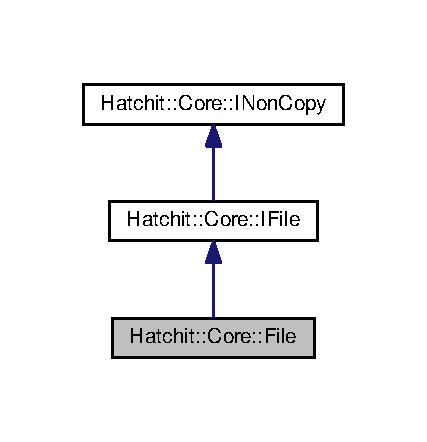
\includegraphics[width=205pt]{classHatchit_1_1Core_1_1File__inherit__graph}
\end{center}
\end{figure}


Collaboration diagram for Hatchit\+:\+:Core\+:\+:File\+:
\nopagebreak
\begin{figure}[H]
\begin{center}
\leavevmode
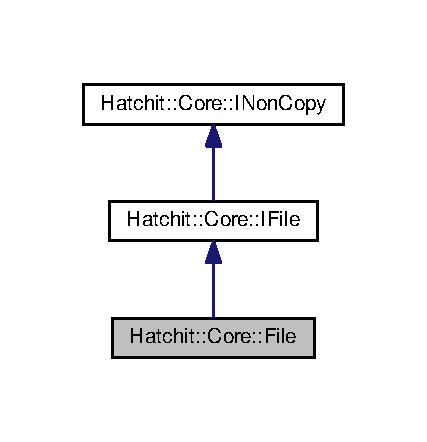
\includegraphics[width=205pt]{classHatchit_1_1Core_1_1File__coll__graph}
\end{center}
\end{figure}
\subsection*{Public Member Functions}
\begin{DoxyCompactItemize}
\item 
virtual std\+::string \hyperlink{classHatchit_1_1Core_1_1File_acf299b9ad7d5362e69ce5e2da1613887}{Name} (void) override
\begin{DoxyCompactList}\small\item\em Returns the name of the file. \end{DoxyCompactList}\item 
virtual std\+::string \hyperlink{classHatchit_1_1Core_1_1File_ad7c6f4473dba9f55fa06095180e8b49f}{Path} (void) override
\begin{DoxyCompactList}\small\item\em Returns the path to the file. \end{DoxyCompactList}\item 
virtual std\+::string \hyperlink{classHatchit_1_1Core_1_1File_a59e1437b18943479de2f6c4234b3eb40}{Base\+Name} (void) override
\begin{DoxyCompactList}\small\item\em Returns the base name of the system file. \end{DoxyCompactList}\item 
virtual void \hyperlink{classHatchit_1_1Core_1_1File_a86b433cd9a4c10cad0bdacba9d4ae770}{Open} (const std\+::string \&path, File\+Mode mode) override
\begin{DoxyCompactList}\small\item\em Opens the file at the given path, using the given File\+Mode. \end{DoxyCompactList}\item 
virtual bool \hyperlink{classHatchit_1_1Core_1_1File_a3cf429a1d4538e301b74fad16e4b5c88}{Seek} (long pos, File\+Seek mode) override
\begin{DoxyCompactList}\small\item\em Moves file stream pointer to requested offset relative to given mode. \end{DoxyCompactList}\item 
virtual size\+\_\+t \hyperlink{classHatchit_1_1Core_1_1File_aa301dd426e9787589b2fcfce6fb25a15}{Read} (B\+Y\+TE $\ast$out, size\+\_\+t len) override
\begin{DoxyCompactList}\small\item\em Reads contents of file into given byte buffer. \end{DoxyCompactList}\item 
virtual size\+\_\+t \hyperlink{classHatchit_1_1Core_1_1File_adca0370e5faf5e22b6b4c5993ae71e5d}{Write} (const B\+Y\+TE $\ast$in, size\+\_\+t len) override
\begin{DoxyCompactList}\small\item\em Writes contents of byte array into file output stream. \end{DoxyCompactList}\item 
virtual bool \hyperlink{classHatchit_1_1Core_1_1File_ae1a078ed489dd57396e53bcd61cbb8c0}{Close} (void) override
\begin{DoxyCompactList}\small\item\em Closes current file and releases memory held from file. \end{DoxyCompactList}\item 
virtual size\+\_\+t \hyperlink{classHatchit_1_1Core_1_1File_af28f52fda6efcbc6b452c8eef7843556}{Tell} (void) override
\begin{DoxyCompactList}\small\item\em Gives current position of stream in file. \end{DoxyCompactList}\item 
virtual size\+\_\+t \hyperlink{classHatchit_1_1Core_1_1File_a179bf2bab450ad8b7808c367b68cfcdc}{Size\+Bytes} (void) override
\begin{DoxyCompactList}\small\item\em Gives size of file in bytes. \end{DoxyCompactList}\item 
virtual size\+\_\+t \hyperlink{classHatchit_1_1Core_1_1File_a3d88ad1d8573c2b78cbd67fac6fd694f}{Size\+K\+Bytes} (void) override
\begin{DoxyCompactList}\small\item\em Gives size of file in Kilobytes. \end{DoxyCompactList}\item 
virtual size\+\_\+t \hyperlink{classHatchit_1_1Core_1_1File_ae19d803e3e7112ef1fb390c101228be6}{Position} (void) override
\begin{DoxyCompactList}\small\item\em Returns position of stream pointer in file. \end{DoxyCompactList}\item 
virtual std\+::fstream $\ast$ \hyperlink{classHatchit_1_1Core_1_1File_a4c29391e00c45e1af2abc45ddd458812}{Handle} (void) override
\begin{DoxyCompactList}\small\item\em Gives file pointer to opened file. \end{DoxyCompactList}\end{DoxyCompactItemize}
\subsection*{Additional Inherited Members}


\subsection{Detailed Description}
Defines a simple \hyperlink{classHatchit_1_1Core_1_1File}{File} class for file input/output. 

Definition at line 34 of file ht\+\_\+file.\+h.



\subsection{Member Function Documentation}
\index{Hatchit\+::\+Core\+::\+File@{Hatchit\+::\+Core\+::\+File}!Base\+Name@{Base\+Name}}
\index{Base\+Name@{Base\+Name}!Hatchit\+::\+Core\+::\+File@{Hatchit\+::\+Core\+::\+File}}
\subsubsection[{\texorpdfstring{Base\+Name(void) override}{BaseName(void) override}}]{\setlength{\rightskip}{0pt plus 5cm}virtual std\+::string Hatchit\+::\+Core\+::\+File\+::\+Base\+Name (
\begin{DoxyParamCaption}
\item[{void}]{}
\end{DoxyParamCaption}
)\hspace{0.3cm}{\ttfamily [override]}, {\ttfamily [virtual]}}\hypertarget{classHatchit_1_1Core_1_1File_a59e1437b18943479de2f6c4234b3eb40}{}\label{classHatchit_1_1Core_1_1File_a59e1437b18943479de2f6c4234b3eb40}


Returns the base name of the system file. 

Returns the base name of the system file open. Base name is the name of the file without the extension. 

Implements \hyperlink{classHatchit_1_1Core_1_1IFile_a9c62bd232c9cce46ccf39d864a816e56}{Hatchit\+::\+Core\+::\+I\+File}.

\index{Hatchit\+::\+Core\+::\+File@{Hatchit\+::\+Core\+::\+File}!Close@{Close}}
\index{Close@{Close}!Hatchit\+::\+Core\+::\+File@{Hatchit\+::\+Core\+::\+File}}
\subsubsection[{\texorpdfstring{Close(void) override}{Close(void) override}}]{\setlength{\rightskip}{0pt plus 5cm}virtual bool Hatchit\+::\+Core\+::\+File\+::\+Close (
\begin{DoxyParamCaption}
\item[{void}]{}
\end{DoxyParamCaption}
)\hspace{0.3cm}{\ttfamily [override]}, {\ttfamily [virtual]}}\hypertarget{classHatchit_1_1Core_1_1File_ae1a078ed489dd57396e53bcd61cbb8c0}{}\label{classHatchit_1_1Core_1_1File_ae1a078ed489dd57396e53bcd61cbb8c0}


Closes current file and releases memory held from file. 

Function closes the currently open file and releases any memory from the file. This function M\+U\+ST be called before destruction of \hyperlink{classHatchit_1_1Core_1_1File}{File} objects. \begin{DoxyReturn}{Returns}
Whether file was successfully closed or not. 
\end{DoxyReturn}


Implements \hyperlink{classHatchit_1_1Core_1_1IFile_a3e604bf80e604d22adfd10475693213e}{Hatchit\+::\+Core\+::\+I\+File}.

\index{Hatchit\+::\+Core\+::\+File@{Hatchit\+::\+Core\+::\+File}!Handle@{Handle}}
\index{Handle@{Handle}!Hatchit\+::\+Core\+::\+File@{Hatchit\+::\+Core\+::\+File}}
\subsubsection[{\texorpdfstring{Handle(void) override}{Handle(void) override}}]{\setlength{\rightskip}{0pt plus 5cm}virtual std\+::fstream$\ast$ Hatchit\+::\+Core\+::\+File\+::\+Handle (
\begin{DoxyParamCaption}
\item[{void}]{}
\end{DoxyParamCaption}
)\hspace{0.3cm}{\ttfamily [override]}, {\ttfamily [virtual]}}\hypertarget{classHatchit_1_1Core_1_1File_a4c29391e00c45e1af2abc45ddd458812}{}\label{classHatchit_1_1Core_1_1File_a4c29391e00c45e1af2abc45ddd458812}


Gives file pointer to opened file. 

Gives file pointer to opened file. 

Implements \hyperlink{classHatchit_1_1Core_1_1IFile_aa9673f333160b5d2b75f1800fb950b21}{Hatchit\+::\+Core\+::\+I\+File}.

\index{Hatchit\+::\+Core\+::\+File@{Hatchit\+::\+Core\+::\+File}!Name@{Name}}
\index{Name@{Name}!Hatchit\+::\+Core\+::\+File@{Hatchit\+::\+Core\+::\+File}}
\subsubsection[{\texorpdfstring{Name(void) override}{Name(void) override}}]{\setlength{\rightskip}{0pt plus 5cm}virtual std\+::string Hatchit\+::\+Core\+::\+File\+::\+Name (
\begin{DoxyParamCaption}
\item[{void}]{}
\end{DoxyParamCaption}
)\hspace{0.3cm}{\ttfamily [override]}, {\ttfamily [virtual]}}\hypertarget{classHatchit_1_1Core_1_1File_acf299b9ad7d5362e69ce5e2da1613887}{}\label{classHatchit_1_1Core_1_1File_acf299b9ad7d5362e69ce5e2da1613887}


Returns the name of the file. 

Returns the name of the file, i.\+e. File\+Name.\+txt 

Implements \hyperlink{classHatchit_1_1Core_1_1IFile_ac60ac0b57e7af8ca509723be55e4638b}{Hatchit\+::\+Core\+::\+I\+File}.

\index{Hatchit\+::\+Core\+::\+File@{Hatchit\+::\+Core\+::\+File}!Open@{Open}}
\index{Open@{Open}!Hatchit\+::\+Core\+::\+File@{Hatchit\+::\+Core\+::\+File}}
\subsubsection[{\texorpdfstring{Open(const std\+::string \&path, File\+Mode mode) override}{Open(const std::string &path, FileMode mode) override}}]{\setlength{\rightskip}{0pt plus 5cm}virtual void Hatchit\+::\+Core\+::\+File\+::\+Open (
\begin{DoxyParamCaption}
\item[{const std\+::string \&}]{path, }
\item[{File\+Mode}]{mode}
\end{DoxyParamCaption}
)\hspace{0.3cm}{\ttfamily [override]}, {\ttfamily [virtual]}}\hypertarget{classHatchit_1_1Core_1_1File_a86b433cd9a4c10cad0bdacba9d4ae770}{}\label{classHatchit_1_1Core_1_1File_a86b433cd9a4c10cad0bdacba9d4ae770}


Opens the file at the given path, using the given File\+Mode. 

Opens the file at the given relative path. Then populates member data with information about the open file. 

Implements \hyperlink{classHatchit_1_1Core_1_1IFile_af5b39a1db2e3e03ebb2a641fed60ea63}{Hatchit\+::\+Core\+::\+I\+File}.

\index{Hatchit\+::\+Core\+::\+File@{Hatchit\+::\+Core\+::\+File}!Path@{Path}}
\index{Path@{Path}!Hatchit\+::\+Core\+::\+File@{Hatchit\+::\+Core\+::\+File}}
\subsubsection[{\texorpdfstring{Path(void) override}{Path(void) override}}]{\setlength{\rightskip}{0pt plus 5cm}virtual std\+::string Hatchit\+::\+Core\+::\+File\+::\+Path (
\begin{DoxyParamCaption}
\item[{void}]{}
\end{DoxyParamCaption}
)\hspace{0.3cm}{\ttfamily [override]}, {\ttfamily [virtual]}}\hypertarget{classHatchit_1_1Core_1_1File_ad7c6f4473dba9f55fa06095180e8b49f}{}\label{classHatchit_1_1Core_1_1File_ad7c6f4473dba9f55fa06095180e8b49f}


Returns the path to the file. 

Returns the relative path to the file. Path includes file name appended to end. 

Implements \hyperlink{classHatchit_1_1Core_1_1IFile_a718f7b7b6ad27be36f1b224ac1254a66}{Hatchit\+::\+Core\+::\+I\+File}.

\index{Hatchit\+::\+Core\+::\+File@{Hatchit\+::\+Core\+::\+File}!Position@{Position}}
\index{Position@{Position}!Hatchit\+::\+Core\+::\+File@{Hatchit\+::\+Core\+::\+File}}
\subsubsection[{\texorpdfstring{Position(void) override}{Position(void) override}}]{\setlength{\rightskip}{0pt plus 5cm}virtual size\+\_\+t Hatchit\+::\+Core\+::\+File\+::\+Position (
\begin{DoxyParamCaption}
\item[{void}]{}
\end{DoxyParamCaption}
)\hspace{0.3cm}{\ttfamily [override]}, {\ttfamily [virtual]}}\hypertarget{classHatchit_1_1Core_1_1File_ae19d803e3e7112ef1fb390c101228be6}{}\label{classHatchit_1_1Core_1_1File_ae19d803e3e7112ef1fb390c101228be6}


Returns position of stream pointer in file. 

Returns position of stream pointer in file (relative to beginning of file). 

Implements \hyperlink{classHatchit_1_1Core_1_1IFile_aa03495bd6404a082c0b0fe53c7e383d0}{Hatchit\+::\+Core\+::\+I\+File}.

\index{Hatchit\+::\+Core\+::\+File@{Hatchit\+::\+Core\+::\+File}!Read@{Read}}
\index{Read@{Read}!Hatchit\+::\+Core\+::\+File@{Hatchit\+::\+Core\+::\+File}}
\subsubsection[{\texorpdfstring{Read(\+B\+Y\+T\+E $\ast$out, size\+\_\+t len) override}{Read(BYTE *out, size_t len) override}}]{\setlength{\rightskip}{0pt plus 5cm}virtual size\+\_\+t Hatchit\+::\+Core\+::\+File\+::\+Read (
\begin{DoxyParamCaption}
\item[{B\+Y\+TE $\ast$}]{out, }
\item[{size\+\_\+t}]{length}
\end{DoxyParamCaption}
)\hspace{0.3cm}{\ttfamily [override]}, {\ttfamily [virtual]}}\hypertarget{classHatchit_1_1Core_1_1File_aa301dd426e9787589b2fcfce6fb25a15}{}\label{classHatchit_1_1Core_1_1File_aa301dd426e9787589b2fcfce6fb25a15}


Reads contents of file into given byte buffer. 

Function reads data from file (based on its current stream pointer position) and places data into given byte buffer, for a maximum of {\itshape length} number of bytes \begin{DoxyReturn}{Returns}
Number of bytes read into byte array. 
\end{DoxyReturn}


Implements \hyperlink{classHatchit_1_1Core_1_1IFile_ab6270f8bde6a526cce3f3a2838bb1331}{Hatchit\+::\+Core\+::\+I\+File}.

\index{Hatchit\+::\+Core\+::\+File@{Hatchit\+::\+Core\+::\+File}!Seek@{Seek}}
\index{Seek@{Seek}!Hatchit\+::\+Core\+::\+File@{Hatchit\+::\+Core\+::\+File}}
\subsubsection[{\texorpdfstring{Seek(long pos, File\+Seek mode) override}{Seek(long pos, FileSeek mode) override}}]{\setlength{\rightskip}{0pt plus 5cm}virtual bool Hatchit\+::\+Core\+::\+File\+::\+Seek (
\begin{DoxyParamCaption}
\item[{long}]{offset, }
\item[{File\+Seek}]{mode}
\end{DoxyParamCaption}
)\hspace{0.3cm}{\ttfamily [override]}, {\ttfamily [virtual]}}\hypertarget{classHatchit_1_1Core_1_1File_a3cf429a1d4538e301b74fad16e4b5c88}{}\label{classHatchit_1_1Core_1_1File_a3cf429a1d4538e301b74fad16e4b5c88}


Moves file stream pointer to requested offset relative to given mode. 

Function moves the stream pointer to a new location, with an offset relative to the given File\+Seek enum. \begin{DoxyReturn}{Returns}
Whether seeked position was found and moved to. 
\end{DoxyReturn}


Implements \hyperlink{classHatchit_1_1Core_1_1IFile_aaf302f7b42b30af0c1827814d805098b}{Hatchit\+::\+Core\+::\+I\+File}.

\index{Hatchit\+::\+Core\+::\+File@{Hatchit\+::\+Core\+::\+File}!Size\+Bytes@{Size\+Bytes}}
\index{Size\+Bytes@{Size\+Bytes}!Hatchit\+::\+Core\+::\+File@{Hatchit\+::\+Core\+::\+File}}
\subsubsection[{\texorpdfstring{Size\+Bytes(void) override}{SizeBytes(void) override}}]{\setlength{\rightskip}{0pt plus 5cm}virtual size\+\_\+t Hatchit\+::\+Core\+::\+File\+::\+Size\+Bytes (
\begin{DoxyParamCaption}
\item[{void}]{}
\end{DoxyParamCaption}
)\hspace{0.3cm}{\ttfamily [override]}, {\ttfamily [virtual]}}\hypertarget{classHatchit_1_1Core_1_1File_a179bf2bab450ad8b7808c367b68cfcdc}{}\label{classHatchit_1_1Core_1_1File_a179bf2bab450ad8b7808c367b68cfcdc}


Gives size of file in bytes. 

Gives size of file in bytes. 

Implements \hyperlink{classHatchit_1_1Core_1_1IFile_a804338c824b2cb4047e45a6b9b62b910}{Hatchit\+::\+Core\+::\+I\+File}.

\index{Hatchit\+::\+Core\+::\+File@{Hatchit\+::\+Core\+::\+File}!Size\+K\+Bytes@{Size\+K\+Bytes}}
\index{Size\+K\+Bytes@{Size\+K\+Bytes}!Hatchit\+::\+Core\+::\+File@{Hatchit\+::\+Core\+::\+File}}
\subsubsection[{\texorpdfstring{Size\+K\+Bytes(void) override}{SizeKBytes(void) override}}]{\setlength{\rightskip}{0pt plus 5cm}virtual size\+\_\+t Hatchit\+::\+Core\+::\+File\+::\+Size\+K\+Bytes (
\begin{DoxyParamCaption}
\item[{void}]{}
\end{DoxyParamCaption}
)\hspace{0.3cm}{\ttfamily [override]}, {\ttfamily [virtual]}}\hypertarget{classHatchit_1_1Core_1_1File_a3d88ad1d8573c2b78cbd67fac6fd694f}{}\label{classHatchit_1_1Core_1_1File_a3d88ad1d8573c2b78cbd67fac6fd694f}


Gives size of file in Kilobytes. 

Gives size of file in kilobytes 

Implements \hyperlink{classHatchit_1_1Core_1_1IFile_aea3fd028436c4e75967b065d5655ca0b}{Hatchit\+::\+Core\+::\+I\+File}.

\index{Hatchit\+::\+Core\+::\+File@{Hatchit\+::\+Core\+::\+File}!Tell@{Tell}}
\index{Tell@{Tell}!Hatchit\+::\+Core\+::\+File@{Hatchit\+::\+Core\+::\+File}}
\subsubsection[{\texorpdfstring{Tell(void) override}{Tell(void) override}}]{\setlength{\rightskip}{0pt plus 5cm}virtual size\+\_\+t Hatchit\+::\+Core\+::\+File\+::\+Tell (
\begin{DoxyParamCaption}
\item[{void}]{}
\end{DoxyParamCaption}
)\hspace{0.3cm}{\ttfamily [override]}, {\ttfamily [virtual]}}\hypertarget{classHatchit_1_1Core_1_1File_af28f52fda6efcbc6b452c8eef7843556}{}\label{classHatchit_1_1Core_1_1File_af28f52fda6efcbc6b452c8eef7843556}


Gives current position of stream in file. 

Function returns the current position of the stream reader relative to the beginning of the file.

\begin{DoxyNote}{Note}
Tell will be more or less arbitrary with text files, but can still be used to return to the same location with \hyperlink{classHatchit_1_1Core_1_1IFile_aaf302f7b42b30af0c1827814d805098b}{I\+File\+::\+Seek(long offset, File\+Seek mode)}; 
\end{DoxyNote}


Implements \hyperlink{classHatchit_1_1Core_1_1IFile_aaa6d3d85bfbbb1edb19be32e8cf271c4}{Hatchit\+::\+Core\+::\+I\+File}.

\index{Hatchit\+::\+Core\+::\+File@{Hatchit\+::\+Core\+::\+File}!Write@{Write}}
\index{Write@{Write}!Hatchit\+::\+Core\+::\+File@{Hatchit\+::\+Core\+::\+File}}
\subsubsection[{\texorpdfstring{Write(const B\+Y\+T\+E $\ast$in, size\+\_\+t len) override}{Write(const BYTE *in, size_t len) override}}]{\setlength{\rightskip}{0pt plus 5cm}virtual size\+\_\+t Hatchit\+::\+Core\+::\+File\+::\+Write (
\begin{DoxyParamCaption}
\item[{const B\+Y\+TE $\ast$}]{in, }
\item[{size\+\_\+t}]{len}
\end{DoxyParamCaption}
)\hspace{0.3cm}{\ttfamily [override]}, {\ttfamily [virtual]}}\hypertarget{classHatchit_1_1Core_1_1File_adca0370e5faf5e22b6b4c5993ae71e5d}{}\label{classHatchit_1_1Core_1_1File_adca0370e5faf5e22b6b4c5993ae71e5d}


Writes contents of byte array into file output stream. 

Function writes contents of given byte array into the file\textquotesingle{}s output stream. The function will write up to a maximum of {\itshape len} bytes. \begin{DoxyReturn}{Returns}
Number of bytes written to file. 
\end{DoxyReturn}


Implements \hyperlink{classHatchit_1_1Core_1_1IFile_a227ad957bbc544111b84871cdc0c2c32}{Hatchit\+::\+Core\+::\+I\+File}.



The documentation for this class was generated from the following file\+:\begin{DoxyCompactItemize}
\item 
/home/debunez/\+Git\+Hub/\+Hatchit\+Editor/\+Hatchit/\+Hatchit\+Core/include/ht\+\_\+file.\+h\end{DoxyCompactItemize}

\hypertarget{classHatchit_1_1Core_1_1FileException}{}\section{Hatchit\+:\+:Core\+:\+:File\+Exception Class Reference}
\label{classHatchit_1_1Core_1_1FileException}\index{Hatchit\+::\+Core\+::\+File\+Exception@{Hatchit\+::\+Core\+::\+File\+Exception}}


Inheritance diagram for Hatchit\+:\+:Core\+:\+:File\+Exception\+:
\nopagebreak
\begin{figure}[H]
\begin{center}
\leavevmode
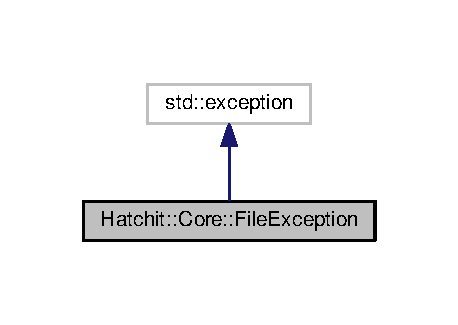
\includegraphics[width=220pt]{classHatchit_1_1Core_1_1FileException__inherit__graph}
\end{center}
\end{figure}


Collaboration diagram for Hatchit\+:\+:Core\+:\+:File\+Exception\+:
\nopagebreak
\begin{figure}[H]
\begin{center}
\leavevmode
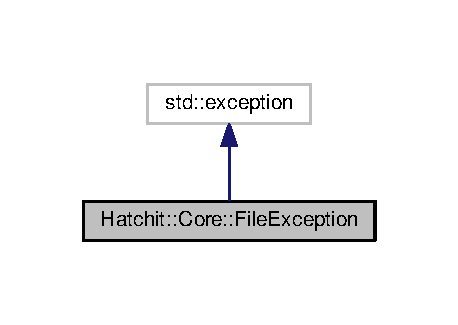
\includegraphics[width=220pt]{classHatchit_1_1Core_1_1FileException__coll__graph}
\end{center}
\end{figure}
\subsection*{Public Member Functions}
\begin{DoxyCompactItemize}
\item 
{\bfseries File\+Exception} (std\+::string file, int error)\hypertarget{classHatchit_1_1Core_1_1FileException_a459566d7214d937f1faeb98d9b958eaf}{}\label{classHatchit_1_1Core_1_1FileException_a459566d7214d937f1faeb98d9b958eaf}

\item 
virtual const char $\ast$ {\bfseries what} () const N\+O\+E\+X\+C\+E\+PT override\hypertarget{classHatchit_1_1Core_1_1FileException_a9d807e97f58efd4e00fb89b1b9c88e9a}{}\label{classHatchit_1_1Core_1_1FileException_a9d807e97f58efd4e00fb89b1b9c88e9a}

\end{DoxyCompactItemize}


\subsection{Detailed Description}


Definition at line 25 of file ht\+\_\+file\+\_\+exception.\+h.



The documentation for this class was generated from the following file\+:\begin{DoxyCompactItemize}
\item 
/home/debunez/\+Git\+Hub/\+Hatchit\+Editor/\+Hatchit/\+Hatchit\+Core/include/ht\+\_\+file\+\_\+exception.\+h\end{DoxyCompactItemize}

\hypertarget{classHatchit_1_1Core_1_1IFile}{}\section{Hatchit\+:\+:Core\+:\+:I\+File Interface Reference}
\label{classHatchit_1_1Core_1_1IFile}\index{Hatchit\+::\+Core\+::\+I\+File@{Hatchit\+::\+Core\+::\+I\+File}}


An interface to describe system files.  




{\ttfamily \#include $<$ht\+\_\+file\+\_\+interface.\+h$>$}



Inheritance diagram for Hatchit\+:\+:Core\+:\+:I\+File\+:
\nopagebreak
\begin{figure}[H]
\begin{center}
\leavevmode
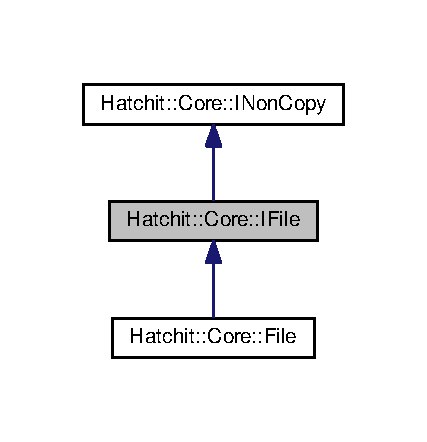
\includegraphics[width=205pt]{classHatchit_1_1Core_1_1IFile__inherit__graph}
\end{center}
\end{figure}


Collaboration diagram for Hatchit\+:\+:Core\+:\+:I\+File\+:
\nopagebreak
\begin{figure}[H]
\begin{center}
\leavevmode
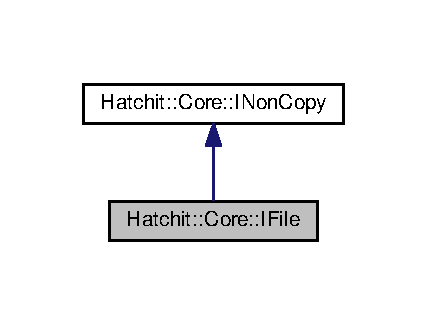
\includegraphics[width=205pt]{classHatchit_1_1Core_1_1IFile__coll__graph}
\end{center}
\end{figure}
\subsection*{Public Types}
\begin{DoxyCompactItemize}
\item 
enum {\bfseries File\+Seek} \{ {\bfseries Current}, 
{\bfseries End}, 
{\bfseries Set}
 \}\hypertarget{classHatchit_1_1Core_1_1IFile_a4fa08027e9a6d42857a363ae63d4aeb6}{}\label{classHatchit_1_1Core_1_1IFile_a4fa08027e9a6d42857a363ae63d4aeb6}

\item 
enum {\bfseries File\+Mode} \{ \\*
{\bfseries Read\+Text}, 
{\bfseries Read\+Binary}, 
{\bfseries Write\+Text}, 
{\bfseries Write\+Binary}, 
\\*
{\bfseries Append\+Text}, 
{\bfseries Append\+Binary}
 \}\hypertarget{classHatchit_1_1Core_1_1IFile_aecd13e31816da4215e320df27f5b4daf}{}\label{classHatchit_1_1Core_1_1IFile_aecd13e31816da4215e320df27f5b4daf}

\end{DoxyCompactItemize}
\subsection*{Public Member Functions}
\begin{DoxyCompactItemize}
\item 
virtual \hyperlink{classHatchit_1_1Core_1_1IFile_a751bf55568c01c776beb115f76b7a929}{$\sim$\+I\+File} ()=default
\begin{DoxyCompactList}\small\item\em Default destructor. \end{DoxyCompactList}\item 
virtual std\+::string \hyperlink{classHatchit_1_1Core_1_1IFile_ac60ac0b57e7af8ca509723be55e4638b}{Name} (void)=0
\begin{DoxyCompactList}\small\item\em Returns the name of the file. \end{DoxyCompactList}\item 
virtual std\+::string \hyperlink{classHatchit_1_1Core_1_1IFile_a718f7b7b6ad27be36f1b224ac1254a66}{Path} (void)=0
\begin{DoxyCompactList}\small\item\em Returns the path to the file. \end{DoxyCompactList}\item 
virtual std\+::string \hyperlink{classHatchit_1_1Core_1_1IFile_a9c62bd232c9cce46ccf39d864a816e56}{Base\+Name} (void)=0
\begin{DoxyCompactList}\small\item\em Returns the base name of the system file. \end{DoxyCompactList}\item 
virtual void \hyperlink{classHatchit_1_1Core_1_1IFile_af5b39a1db2e3e03ebb2a641fed60ea63}{Open} (const std\+::string \&path, File\+Mode mode)=0
\begin{DoxyCompactList}\small\item\em Opens the file at the given path, using the given File\+Mode. \end{DoxyCompactList}\item 
virtual bool \hyperlink{classHatchit_1_1Core_1_1IFile_aaf302f7b42b30af0c1827814d805098b}{Seek} (long offset, File\+Seek mode)=0
\begin{DoxyCompactList}\small\item\em Moves file stream pointer to requested offset relative to given mode. \end{DoxyCompactList}\item 
virtual bool \hyperlink{classHatchit_1_1Core_1_1IFile_a3e604bf80e604d22adfd10475693213e}{Close} (void)=0
\begin{DoxyCompactList}\small\item\em Closes current file and releases memory held from file. \end{DoxyCompactList}\item 
virtual size\+\_\+t \hyperlink{classHatchit_1_1Core_1_1IFile_ab6270f8bde6a526cce3f3a2838bb1331}{Read} (B\+Y\+TE $\ast$out, size\+\_\+t len)=0
\begin{DoxyCompactList}\small\item\em Reads contents of file into given byte buffer. \end{DoxyCompactList}\item 
virtual size\+\_\+t \hyperlink{classHatchit_1_1Core_1_1IFile_a227ad957bbc544111b84871cdc0c2c32}{Write} (const B\+Y\+TE $\ast$in, size\+\_\+t len)=0
\begin{DoxyCompactList}\small\item\em Writes contents of byte array into file output stream. \end{DoxyCompactList}\item 
virtual size\+\_\+t \hyperlink{classHatchit_1_1Core_1_1IFile_aaa6d3d85bfbbb1edb19be32e8cf271c4}{Tell} (void)=0
\begin{DoxyCompactList}\small\item\em Gives current position of stream in file. \end{DoxyCompactList}\item 
virtual size\+\_\+t \hyperlink{classHatchit_1_1Core_1_1IFile_a804338c824b2cb4047e45a6b9b62b910}{Size\+Bytes} (void)=0
\begin{DoxyCompactList}\small\item\em Gives size of file in bytes. \end{DoxyCompactList}\item 
virtual size\+\_\+t \hyperlink{classHatchit_1_1Core_1_1IFile_aea3fd028436c4e75967b065d5655ca0b}{Size\+K\+Bytes} (void)=0
\begin{DoxyCompactList}\small\item\em Gives size of file in Kilobytes. \end{DoxyCompactList}\item 
virtual size\+\_\+t \hyperlink{classHatchit_1_1Core_1_1IFile_aa03495bd6404a082c0b0fe53c7e383d0}{Position} (void)=0
\begin{DoxyCompactList}\small\item\em Returns position of stream pointer in file. \end{DoxyCompactList}\item 
virtual std\+::fstream $\ast$ \hyperlink{classHatchit_1_1Core_1_1IFile_aa9673f333160b5d2b75f1800fb950b21}{Handle} ()=0
\begin{DoxyCompactList}\small\item\em Gives file pointer to opened file. \end{DoxyCompactList}\end{DoxyCompactItemize}
\subsection*{Additional Inherited Members}


\subsection{Detailed Description}
An interface to describe system files. 

Interface describes the common functionality of files. 

Definition at line 35 of file ht\+\_\+file\+\_\+interface.\+h.



\subsection{Constructor \& Destructor Documentation}
\index{Hatchit\+::\+Core\+::\+I\+File@{Hatchit\+::\+Core\+::\+I\+File}!````~I\+File@{$\sim$\+I\+File}}
\index{````~I\+File@{$\sim$\+I\+File}!Hatchit\+::\+Core\+::\+I\+File@{Hatchit\+::\+Core\+::\+I\+File}}
\subsubsection[{\texorpdfstring{$\sim$\+I\+File()=default}{~IFile()=default}}]{\setlength{\rightskip}{0pt plus 5cm}Hatchit\+::\+Core\+::\+I\+File\+::$\sim$\+I\+File (
\begin{DoxyParamCaption}
{}
\end{DoxyParamCaption}
)\hspace{0.3cm}{\ttfamily [virtual]}, {\ttfamily [default]}}\hypertarget{classHatchit_1_1Core_1_1IFile_a751bf55568c01c776beb115f76b7a929}{}\label{classHatchit_1_1Core_1_1IFile_a751bf55568c01c776beb115f76b7a929}


Default destructor. 

Default destructor 

\subsection{Member Function Documentation}
\index{Hatchit\+::\+Core\+::\+I\+File@{Hatchit\+::\+Core\+::\+I\+File}!Base\+Name@{Base\+Name}}
\index{Base\+Name@{Base\+Name}!Hatchit\+::\+Core\+::\+I\+File@{Hatchit\+::\+Core\+::\+I\+File}}
\subsubsection[{\texorpdfstring{Base\+Name(void)=0}{BaseName(void)=0}}]{\setlength{\rightskip}{0pt plus 5cm}std\+::string Hatchit\+::\+Core\+::\+I\+File\+::\+Base\+Name (
\begin{DoxyParamCaption}
\item[{void}]{}
\end{DoxyParamCaption}
)\hspace{0.3cm}{\ttfamily [pure virtual]}}\hypertarget{classHatchit_1_1Core_1_1IFile_a9c62bd232c9cce46ccf39d864a816e56}{}\label{classHatchit_1_1Core_1_1IFile_a9c62bd232c9cce46ccf39d864a816e56}


Returns the base name of the system file. 

Returns the base name of the system file open. Base name is the name of the file without the extension. 

Implemented in \hyperlink{classHatchit_1_1Core_1_1File_a59e1437b18943479de2f6c4234b3eb40}{Hatchit\+::\+Core\+::\+File}.

\index{Hatchit\+::\+Core\+::\+I\+File@{Hatchit\+::\+Core\+::\+I\+File}!Close@{Close}}
\index{Close@{Close}!Hatchit\+::\+Core\+::\+I\+File@{Hatchit\+::\+Core\+::\+I\+File}}
\subsubsection[{\texorpdfstring{Close(void)=0}{Close(void)=0}}]{\setlength{\rightskip}{0pt plus 5cm}bool Hatchit\+::\+Core\+::\+I\+File\+::\+Close (
\begin{DoxyParamCaption}
\item[{void}]{}
\end{DoxyParamCaption}
)\hspace{0.3cm}{\ttfamily [pure virtual]}}\hypertarget{classHatchit_1_1Core_1_1IFile_a3e604bf80e604d22adfd10475693213e}{}\label{classHatchit_1_1Core_1_1IFile_a3e604bf80e604d22adfd10475693213e}


Closes current file and releases memory held from file. 

Function closes the currently open file and releases any memory from the file. This function M\+U\+ST be called before destruction of \hyperlink{classHatchit_1_1Core_1_1File}{File} objects. \begin{DoxyReturn}{Returns}
Whether file was successfully closed or not. 
\end{DoxyReturn}


Implemented in \hyperlink{classHatchit_1_1Core_1_1File_ae1a078ed489dd57396e53bcd61cbb8c0}{Hatchit\+::\+Core\+::\+File}.

\index{Hatchit\+::\+Core\+::\+I\+File@{Hatchit\+::\+Core\+::\+I\+File}!Handle@{Handle}}
\index{Handle@{Handle}!Hatchit\+::\+Core\+::\+I\+File@{Hatchit\+::\+Core\+::\+I\+File}}
\subsubsection[{\texorpdfstring{Handle()=0}{Handle()=0}}]{\setlength{\rightskip}{0pt plus 5cm}F\+I\+LE $\ast$ Hatchit\+::\+Core\+::\+I\+File\+::\+Handle (
\begin{DoxyParamCaption}
\item[{void}]{}
\end{DoxyParamCaption}
)\hspace{0.3cm}{\ttfamily [pure virtual]}}\hypertarget{classHatchit_1_1Core_1_1IFile_aa9673f333160b5d2b75f1800fb950b21}{}\label{classHatchit_1_1Core_1_1IFile_aa9673f333160b5d2b75f1800fb950b21}


Gives file pointer to opened file. 

Gives file pointer to opened file. 

Implemented in \hyperlink{classHatchit_1_1Core_1_1File_a4c29391e00c45e1af2abc45ddd458812}{Hatchit\+::\+Core\+::\+File}.

\index{Hatchit\+::\+Core\+::\+I\+File@{Hatchit\+::\+Core\+::\+I\+File}!Name@{Name}}
\index{Name@{Name}!Hatchit\+::\+Core\+::\+I\+File@{Hatchit\+::\+Core\+::\+I\+File}}
\subsubsection[{\texorpdfstring{Name(void)=0}{Name(void)=0}}]{\setlength{\rightskip}{0pt plus 5cm}std\+::string Hatchit\+::\+Core\+::\+I\+File\+::\+Name (
\begin{DoxyParamCaption}
\item[{void}]{}
\end{DoxyParamCaption}
)\hspace{0.3cm}{\ttfamily [pure virtual]}}\hypertarget{classHatchit_1_1Core_1_1IFile_ac60ac0b57e7af8ca509723be55e4638b}{}\label{classHatchit_1_1Core_1_1IFile_ac60ac0b57e7af8ca509723be55e4638b}


Returns the name of the file. 

Returns the name of the file, i.\+e. File\+Name.\+txt 

Implemented in \hyperlink{classHatchit_1_1Core_1_1File_acf299b9ad7d5362e69ce5e2da1613887}{Hatchit\+::\+Core\+::\+File}.

\index{Hatchit\+::\+Core\+::\+I\+File@{Hatchit\+::\+Core\+::\+I\+File}!Open@{Open}}
\index{Open@{Open}!Hatchit\+::\+Core\+::\+I\+File@{Hatchit\+::\+Core\+::\+I\+File}}
\subsubsection[{\texorpdfstring{Open(const std\+::string \&path, File\+Mode mode)=0}{Open(const std::string &path, FileMode mode)=0}}]{\setlength{\rightskip}{0pt plus 5cm}void Hatchit\+::\+Core\+::\+I\+File\+::\+Open (
\begin{DoxyParamCaption}
\item[{const std\+::string \&}]{path, }
\item[{File\+Mode}]{mode}
\end{DoxyParamCaption}
)\hspace{0.3cm}{\ttfamily [pure virtual]}}\hypertarget{classHatchit_1_1Core_1_1IFile_af5b39a1db2e3e03ebb2a641fed60ea63}{}\label{classHatchit_1_1Core_1_1IFile_af5b39a1db2e3e03ebb2a641fed60ea63}


Opens the file at the given path, using the given File\+Mode. 

Opens the file at the given relative path. Then populates member data with information about the open file. 

Implemented in \hyperlink{classHatchit_1_1Core_1_1File_a86b433cd9a4c10cad0bdacba9d4ae770}{Hatchit\+::\+Core\+::\+File}.

\index{Hatchit\+::\+Core\+::\+I\+File@{Hatchit\+::\+Core\+::\+I\+File}!Path@{Path}}
\index{Path@{Path}!Hatchit\+::\+Core\+::\+I\+File@{Hatchit\+::\+Core\+::\+I\+File}}
\subsubsection[{\texorpdfstring{Path(void)=0}{Path(void)=0}}]{\setlength{\rightskip}{0pt plus 5cm}std\+::string Hatchit\+::\+Core\+::\+I\+File\+::\+Path (
\begin{DoxyParamCaption}
\item[{void}]{}
\end{DoxyParamCaption}
)\hspace{0.3cm}{\ttfamily [pure virtual]}}\hypertarget{classHatchit_1_1Core_1_1IFile_a718f7b7b6ad27be36f1b224ac1254a66}{}\label{classHatchit_1_1Core_1_1IFile_a718f7b7b6ad27be36f1b224ac1254a66}


Returns the path to the file. 

Returns the relative path to the file. Path includes file name appended to end. 

Implemented in \hyperlink{classHatchit_1_1Core_1_1File_ad7c6f4473dba9f55fa06095180e8b49f}{Hatchit\+::\+Core\+::\+File}.

\index{Hatchit\+::\+Core\+::\+I\+File@{Hatchit\+::\+Core\+::\+I\+File}!Position@{Position}}
\index{Position@{Position}!Hatchit\+::\+Core\+::\+I\+File@{Hatchit\+::\+Core\+::\+I\+File}}
\subsubsection[{\texorpdfstring{Position(void)=0}{Position(void)=0}}]{\setlength{\rightskip}{0pt plus 5cm}size\+\_\+t Hatchit\+::\+Core\+::\+I\+File\+::\+Position (
\begin{DoxyParamCaption}
\item[{void}]{}
\end{DoxyParamCaption}
)\hspace{0.3cm}{\ttfamily [pure virtual]}}\hypertarget{classHatchit_1_1Core_1_1IFile_aa03495bd6404a082c0b0fe53c7e383d0}{}\label{classHatchit_1_1Core_1_1IFile_aa03495bd6404a082c0b0fe53c7e383d0}


Returns position of stream pointer in file. 

Returns position of stream pointer in file (relative to beginning of file). 

Implemented in \hyperlink{classHatchit_1_1Core_1_1File_ae19d803e3e7112ef1fb390c101228be6}{Hatchit\+::\+Core\+::\+File}.

\index{Hatchit\+::\+Core\+::\+I\+File@{Hatchit\+::\+Core\+::\+I\+File}!Read@{Read}}
\index{Read@{Read}!Hatchit\+::\+Core\+::\+I\+File@{Hatchit\+::\+Core\+::\+I\+File}}
\subsubsection[{\texorpdfstring{Read(\+B\+Y\+T\+E $\ast$out, size\+\_\+t len)=0}{Read(BYTE *out, size_t len)=0}}]{\setlength{\rightskip}{0pt plus 5cm}size\+\_\+t Hatchit\+::\+Core\+::\+I\+File\+::\+Read (
\begin{DoxyParamCaption}
\item[{B\+Y\+TE $\ast$}]{out, }
\item[{size\+\_\+t}]{length}
\end{DoxyParamCaption}
)\hspace{0.3cm}{\ttfamily [pure virtual]}}\hypertarget{classHatchit_1_1Core_1_1IFile_ab6270f8bde6a526cce3f3a2838bb1331}{}\label{classHatchit_1_1Core_1_1IFile_ab6270f8bde6a526cce3f3a2838bb1331}


Reads contents of file into given byte buffer. 

Function reads data from file (based on its current stream pointer position) and places data into given byte buffer, for a maximum of {\itshape length} number of bytes \begin{DoxyReturn}{Returns}
Number of bytes read into byte array. 
\end{DoxyReturn}


Implemented in \hyperlink{classHatchit_1_1Core_1_1File_aa301dd426e9787589b2fcfce6fb25a15}{Hatchit\+::\+Core\+::\+File}.

\index{Hatchit\+::\+Core\+::\+I\+File@{Hatchit\+::\+Core\+::\+I\+File}!Seek@{Seek}}
\index{Seek@{Seek}!Hatchit\+::\+Core\+::\+I\+File@{Hatchit\+::\+Core\+::\+I\+File}}
\subsubsection[{\texorpdfstring{Seek(long offset, File\+Seek mode)=0}{Seek(long offset, FileSeek mode)=0}}]{\setlength{\rightskip}{0pt plus 5cm}bool Hatchit\+::\+Core\+::\+I\+File\+::\+Seek (
\begin{DoxyParamCaption}
\item[{long}]{offset, }
\item[{File\+Seek}]{mode}
\end{DoxyParamCaption}
)\hspace{0.3cm}{\ttfamily [pure virtual]}}\hypertarget{classHatchit_1_1Core_1_1IFile_aaf302f7b42b30af0c1827814d805098b}{}\label{classHatchit_1_1Core_1_1IFile_aaf302f7b42b30af0c1827814d805098b}


Moves file stream pointer to requested offset relative to given mode. 

Function moves the stream pointer to a new location, with an offset relative to the given File\+Seek enum. \begin{DoxyReturn}{Returns}
Whether seeked position was found and moved to. 
\end{DoxyReturn}


Implemented in \hyperlink{classHatchit_1_1Core_1_1File_a3cf429a1d4538e301b74fad16e4b5c88}{Hatchit\+::\+Core\+::\+File}.

\index{Hatchit\+::\+Core\+::\+I\+File@{Hatchit\+::\+Core\+::\+I\+File}!Size\+Bytes@{Size\+Bytes}}
\index{Size\+Bytes@{Size\+Bytes}!Hatchit\+::\+Core\+::\+I\+File@{Hatchit\+::\+Core\+::\+I\+File}}
\subsubsection[{\texorpdfstring{Size\+Bytes(void)=0}{SizeBytes(void)=0}}]{\setlength{\rightskip}{0pt plus 5cm}size\+\_\+t Hatchit\+::\+Core\+::\+I\+File\+::\+Size\+Bytes (
\begin{DoxyParamCaption}
\item[{void}]{}
\end{DoxyParamCaption}
)\hspace{0.3cm}{\ttfamily [pure virtual]}}\hypertarget{classHatchit_1_1Core_1_1IFile_a804338c824b2cb4047e45a6b9b62b910}{}\label{classHatchit_1_1Core_1_1IFile_a804338c824b2cb4047e45a6b9b62b910}


Gives size of file in bytes. 

Gives size of file in bytes. 

Implemented in \hyperlink{classHatchit_1_1Core_1_1File_a179bf2bab450ad8b7808c367b68cfcdc}{Hatchit\+::\+Core\+::\+File}.

\index{Hatchit\+::\+Core\+::\+I\+File@{Hatchit\+::\+Core\+::\+I\+File}!Size\+K\+Bytes@{Size\+K\+Bytes}}
\index{Size\+K\+Bytes@{Size\+K\+Bytes}!Hatchit\+::\+Core\+::\+I\+File@{Hatchit\+::\+Core\+::\+I\+File}}
\subsubsection[{\texorpdfstring{Size\+K\+Bytes(void)=0}{SizeKBytes(void)=0}}]{\setlength{\rightskip}{0pt plus 5cm}size\+\_\+t Hatchit\+::\+Core\+::\+I\+File\+::\+Size\+K\+Bytes (
\begin{DoxyParamCaption}
\item[{void}]{}
\end{DoxyParamCaption}
)\hspace{0.3cm}{\ttfamily [pure virtual]}}\hypertarget{classHatchit_1_1Core_1_1IFile_aea3fd028436c4e75967b065d5655ca0b}{}\label{classHatchit_1_1Core_1_1IFile_aea3fd028436c4e75967b065d5655ca0b}


Gives size of file in Kilobytes. 

Gives size of file in kilobytes 

Implemented in \hyperlink{classHatchit_1_1Core_1_1File_a3d88ad1d8573c2b78cbd67fac6fd694f}{Hatchit\+::\+Core\+::\+File}.

\index{Hatchit\+::\+Core\+::\+I\+File@{Hatchit\+::\+Core\+::\+I\+File}!Tell@{Tell}}
\index{Tell@{Tell}!Hatchit\+::\+Core\+::\+I\+File@{Hatchit\+::\+Core\+::\+I\+File}}
\subsubsection[{\texorpdfstring{Tell(void)=0}{Tell(void)=0}}]{\setlength{\rightskip}{0pt plus 5cm}size\+\_\+t Hatchit\+::\+Core\+::\+I\+File\+::\+Tell (
\begin{DoxyParamCaption}
\item[{void}]{}
\end{DoxyParamCaption}
)\hspace{0.3cm}{\ttfamily [pure virtual]}}\hypertarget{classHatchit_1_1Core_1_1IFile_aaa6d3d85bfbbb1edb19be32e8cf271c4}{}\label{classHatchit_1_1Core_1_1IFile_aaa6d3d85bfbbb1edb19be32e8cf271c4}


Gives current position of stream in file. 

Function returns the current position of the stream reader relative to the beginning of the file.

\begin{DoxyNote}{Note}
Tell will be more or less arbitrary with text files, but can still be used to return to the same location with \hyperlink{classHatchit_1_1Core_1_1IFile_aaf302f7b42b30af0c1827814d805098b}{I\+File\+::\+Seek(long offset, File\+Seek mode)}; 
\end{DoxyNote}


Implemented in \hyperlink{classHatchit_1_1Core_1_1File_af28f52fda6efcbc6b452c8eef7843556}{Hatchit\+::\+Core\+::\+File}.

\index{Hatchit\+::\+Core\+::\+I\+File@{Hatchit\+::\+Core\+::\+I\+File}!Write@{Write}}
\index{Write@{Write}!Hatchit\+::\+Core\+::\+I\+File@{Hatchit\+::\+Core\+::\+I\+File}}
\subsubsection[{\texorpdfstring{Write(const B\+Y\+T\+E $\ast$in, size\+\_\+t len)=0}{Write(const BYTE *in, size_t len)=0}}]{\setlength{\rightskip}{0pt plus 5cm}size\+\_\+t Hatchit\+::\+Core\+::\+I\+File\+::\+Write (
\begin{DoxyParamCaption}
\item[{const B\+Y\+TE $\ast$}]{in, }
\item[{size\+\_\+t}]{len}
\end{DoxyParamCaption}
)\hspace{0.3cm}{\ttfamily [pure virtual]}}\hypertarget{classHatchit_1_1Core_1_1IFile_a227ad957bbc544111b84871cdc0c2c32}{}\label{classHatchit_1_1Core_1_1IFile_a227ad957bbc544111b84871cdc0c2c32}


Writes contents of byte array into file output stream. 

Function writes contents of given byte array into the file\textquotesingle{}s output stream. The function will write up to a maximum of {\itshape len} bytes. \begin{DoxyReturn}{Returns}
Number of bytes written to file. 
\end{DoxyReturn}


Implemented in \hyperlink{classHatchit_1_1Core_1_1File_adca0370e5faf5e22b6b4c5993ae71e5d}{Hatchit\+::\+Core\+::\+File}.



The documentation for this interface was generated from the following file\+:\begin{DoxyCompactItemize}
\item 
/home/debunez/\+Git\+Hub/\+Hatchit\+Editor/\+Hatchit/\+Hatchit\+Core/include/ht\+\_\+file\+\_\+interface.\+h\end{DoxyCompactItemize}

\hypertarget{classHatchit_1_1Core_1_1IJob}{}\section{Hatchit\+:\+:Core\+:\+:I\+Job Interface Reference}
\label{classHatchit_1_1Core_1_1IJob}\index{Hatchit\+::\+Core\+::\+I\+Job@{Hatchit\+::\+Core\+::\+I\+Job}}


Interface for threading job.  




{\ttfamily \#include $<$ht\+\_\+scheduler.\+h$>$}



Inheritance diagram for Hatchit\+:\+:Core\+:\+:I\+Job\+:
\nopagebreak
\begin{figure}[H]
\begin{center}
\leavevmode
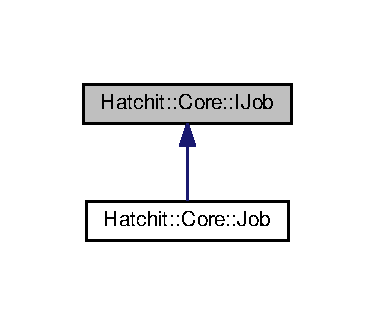
\includegraphics[width=180pt]{classHatchit_1_1Core_1_1IJob__inherit__graph}
\end{center}
\end{figure}
\subsection*{Public Member Functions}
\begin{DoxyCompactItemize}
\item 
virtual std\+::thread {\bfseries Get\+Thread} ()=0\hypertarget{classHatchit_1_1Core_1_1IJob_ad13d0b3a6fc70d275322982e83a021c3}{}\label{classHatchit_1_1Core_1_1IJob_ad13d0b3a6fc70d275322982e83a021c3}

\end{DoxyCompactItemize}


\subsection{Detailed Description}
Interface for threading job. 

Definition at line 43 of file ht\+\_\+scheduler.\+h.



The documentation for this interface was generated from the following file\+:\begin{DoxyCompactItemize}
\item 
/home/debunez/\+Git\+Hub/\+Hatchit\+Editor/\+Hatchit/\+Hatchit\+Core/include/ht\+\_\+scheduler.\+h\end{DoxyCompactItemize}

\hypertarget{classHatchit_1_1Core_1_1INIException}{}\section{Hatchit\+:\+:Core\+:\+:I\+N\+I\+Exception Class Reference}
\label{classHatchit_1_1Core_1_1INIException}\index{Hatchit\+::\+Core\+::\+I\+N\+I\+Exception@{Hatchit\+::\+Core\+::\+I\+N\+I\+Exception}}


Exception for errors reading an I\+NI file.  




{\ttfamily \#include $<$ht\+\_\+ini\+\_\+exception.\+h$>$}



Inheritance diagram for Hatchit\+:\+:Core\+:\+:I\+N\+I\+Exception\+:
\nopagebreak
\begin{figure}[H]
\begin{center}
\leavevmode
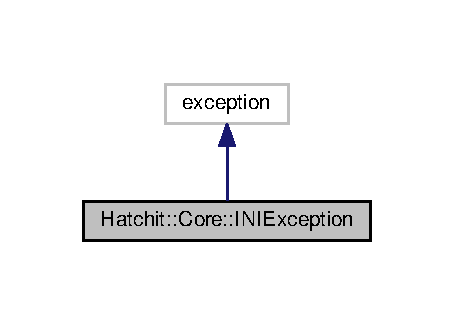
\includegraphics[width=218pt]{classHatchit_1_1Core_1_1INIException__inherit__graph}
\end{center}
\end{figure}


Collaboration diagram for Hatchit\+:\+:Core\+:\+:I\+N\+I\+Exception\+:
\nopagebreak
\begin{figure}[H]
\begin{center}
\leavevmode
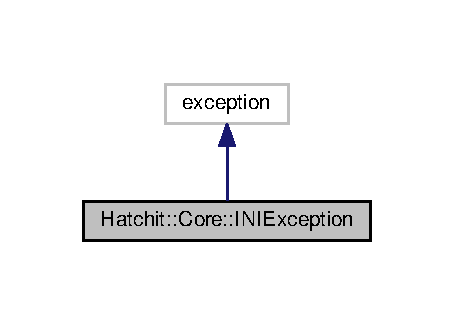
\includegraphics[width=218pt]{classHatchit_1_1Core_1_1INIException__coll__graph}
\end{center}
\end{figure}
\subsection*{Public Member Functions}
\begin{DoxyCompactItemize}
\item 
{\bfseries I\+N\+I\+Exception} (std\+::string name, int error)\hypertarget{classHatchit_1_1Core_1_1INIException_a586d5a44306c53f42adc5453b06f7f5f}{}\label{classHatchit_1_1Core_1_1INIException_a586d5a44306c53f42adc5453b06f7f5f}

\item 
const char $\ast$ {\bfseries what} () const N\+O\+E\+X\+C\+E\+PT override\hypertarget{classHatchit_1_1Core_1_1INIException_a789a6382958ad24e50c0975a298c46a7}{}\label{classHatchit_1_1Core_1_1INIException_a789a6382958ad24e50c0975a298c46a7}

\end{DoxyCompactItemize}


\subsection{Detailed Description}
Exception for errors reading an I\+NI file. 

This exception is thrown during the parsing of an I\+NI file. It gives the file name as well as the type of error it received. 

Definition at line 33 of file ht\+\_\+ini\+\_\+exception.\+h.



The documentation for this class was generated from the following file\+:\begin{DoxyCompactItemize}
\item 
/home/debunez/\+Git\+Hub/\+Hatchit\+Editor/\+Hatchit/\+Hatchit\+Core/include/ht\+\_\+ini\+\_\+exception.\+h\end{DoxyCompactItemize}

\hypertarget{classHatchit_1_1Core_1_1INISettings}{}\section{Hatchit\+:\+:Core\+:\+:I\+N\+I\+Settings Class Reference}
\label{classHatchit_1_1Core_1_1INISettings}\index{Hatchit\+::\+Core\+::\+I\+N\+I\+Settings@{Hatchit\+::\+Core\+::\+I\+N\+I\+Settings}}


Class handling reading and writing of .ini files.  




{\ttfamily \#include $<$ht\+\_\+inisettings.\+h$>$}

\subsection*{Public Member Functions}
\begin{DoxyCompactItemize}
\item 
void {\bfseries Load} (\hyperlink{classHatchit_1_1Core_1_1File}{File} \&file)\hypertarget{classHatchit_1_1Core_1_1INISettings_a8884aa363f6b2919faa681bcb05d0495}{}\label{classHatchit_1_1Core_1_1INISettings_a8884aa363f6b2919faa681bcb05d0495}

\item 
void {\bfseries Write} (\hyperlink{classHatchit_1_1Core_1_1File}{File} \&file)\hypertarget{classHatchit_1_1Core_1_1INISettings_a2d45a3863e18642c10f2bcf7befd3864}{}\label{classHatchit_1_1Core_1_1INISettings_a2d45a3863e18642c10f2bcf7befd3864}

\item 
{\footnotesize template$<$typename T $>$ }\\T {\bfseries Get\+Value} (const std\+::string \&section, const std\+::string \&name)\hypertarget{classHatchit_1_1Core_1_1INISettings_a06689968496fe4210b8410ba1d78e4cc}{}\label{classHatchit_1_1Core_1_1INISettings_a06689968496fe4210b8410ba1d78e4cc}

\item 
{\footnotesize template$<$typename T $>$ }\\void {\bfseries Set\+Value} (const std\+::string \&section, const std\+::string \&name, T value)\hypertarget{classHatchit_1_1Core_1_1INISettings_a62206a2d505564553f8c8d5a1473d00d}{}\label{classHatchit_1_1Core_1_1INISettings_a62206a2d505564553f8c8d5a1473d00d}

\end{DoxyCompactItemize}


\subsection{Detailed Description}
Class handling reading and writing of .ini files. 

Class handles loading and writing .ini files to and from memory. 

Definition at line 49 of file ht\+\_\+inisettings.\+h.



The documentation for this class was generated from the following file\+:\begin{DoxyCompactItemize}
\item 
/home/debunez/\+Git\+Hub/\+Hatchit\+Editor/\+Hatchit/\+Hatchit\+Core/include/ht\+\_\+inisettings.\+h\end{DoxyCompactItemize}

\hypertarget{classHatchit_1_1Core_1_1INonCopy}{}\section{Hatchit\+:\+:Core\+:\+:I\+Non\+Copy Interface Reference}
\label{classHatchit_1_1Core_1_1INonCopy}\index{Hatchit\+::\+Core\+::\+I\+Non\+Copy@{Hatchit\+::\+Core\+::\+I\+Non\+Copy}}


Describes a class that cannot be copied.  




{\ttfamily \#include $<$ht\+\_\+noncopy.\+h$>$}



Inheritance diagram for Hatchit\+:\+:Core\+:\+:I\+Non\+Copy\+:
\nopagebreak
\begin{figure}[H]
\begin{center}
\leavevmode
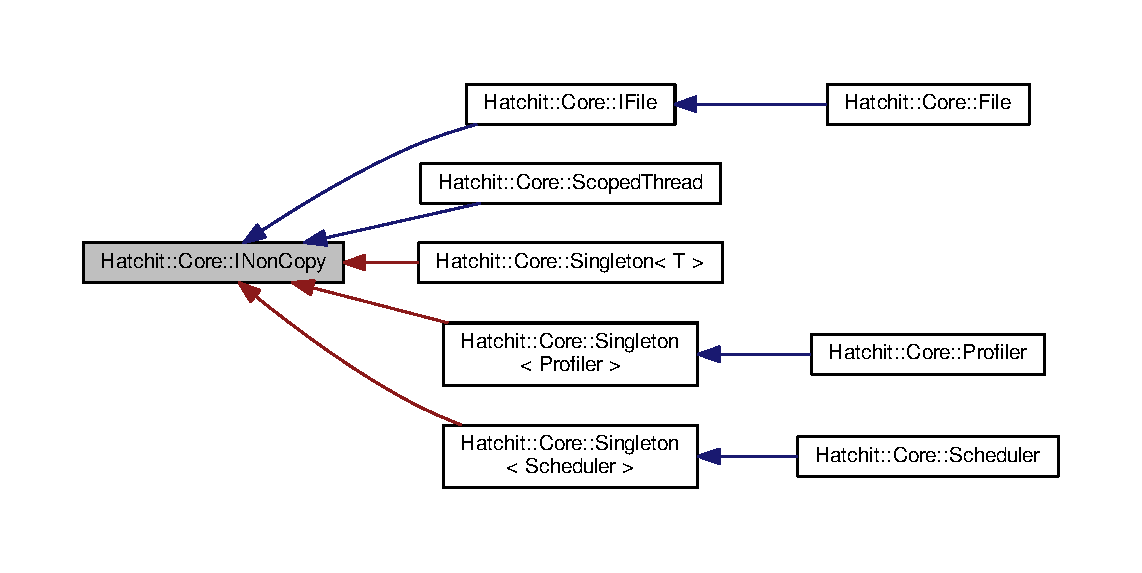
\includegraphics[width=350pt]{classHatchit_1_1Core_1_1INonCopy__inherit__graph}
\end{center}
\end{figure}
\subsection*{Protected Member Functions}
\begin{DoxyCompactItemize}
\item 
{\bfseries I\+Non\+Copy} (const \hyperlink{classHatchit_1_1Core_1_1INonCopy}{I\+Non\+Copy} \&)=delete\hypertarget{classHatchit_1_1Core_1_1INonCopy_a1471227a7ef7a83b800bb27236efd6eb}{}\label{classHatchit_1_1Core_1_1INonCopy_a1471227a7ef7a83b800bb27236efd6eb}

\item 
{\bfseries I\+Non\+Copy} (\hyperlink{classHatchit_1_1Core_1_1INonCopy}{I\+Non\+Copy} \&\&)=default\hypertarget{classHatchit_1_1Core_1_1INonCopy_ab1ba3d28135e594ba7530de7b2369f23}{}\label{classHatchit_1_1Core_1_1INonCopy_ab1ba3d28135e594ba7530de7b2369f23}

\item 
\hyperlink{classHatchit_1_1Core_1_1INonCopy}{I\+Non\+Copy} \& {\bfseries operator=} (const \hyperlink{classHatchit_1_1Core_1_1INonCopy}{I\+Non\+Copy} \&)=delete\hypertarget{classHatchit_1_1Core_1_1INonCopy_a72dca01c3ab5356905dfa436da602673}{}\label{classHatchit_1_1Core_1_1INonCopy_a72dca01c3ab5356905dfa436da602673}

\item 
\hyperlink{classHatchit_1_1Core_1_1INonCopy}{I\+Non\+Copy} \& {\bfseries operator=} (\hyperlink{classHatchit_1_1Core_1_1INonCopy}{I\+Non\+Copy} \&\&)=default\hypertarget{classHatchit_1_1Core_1_1INonCopy_aa87747b247cf108d9c18e9ed7634493d}{}\label{classHatchit_1_1Core_1_1INonCopy_aa87747b247cf108d9c18e9ed7634493d}

\end{DoxyCompactItemize}


\subsection{Detailed Description}
Describes a class that cannot be copied. 

\hyperlink{classHatchit_1_1Core_1_1INonCopy}{I\+Non\+Copy} describes the interface of a non-\/copyable class. Any attempt to copy an \hyperlink{classHatchit_1_1Core_1_1INonCopy}{I\+Non\+Copy} will not compile. 

Definition at line 38 of file ht\+\_\+noncopy.\+h.



The documentation for this interface was generated from the following file\+:\begin{DoxyCompactItemize}
\item 
/home/debunez/\+Git\+Hub/\+Hatchit\+Editor/\+Hatchit/\+Hatchit\+Core/include/\hyperlink{ht__noncopy_8h}{ht\+\_\+noncopy.\+h}\end{DoxyCompactItemize}

\hypertarget{classHatchit_1_1Core_1_1ITimer}{}\section{Hatchit\+:\+:Core\+:\+:I\+Timer Interface Reference}
\label{classHatchit_1_1Core_1_1ITimer}\index{Hatchit\+::\+Core\+::\+I\+Timer@{Hatchit\+::\+Core\+::\+I\+Timer}}


Interface to describe timer functionality.  




{\ttfamily \#include $<$ht\+\_\+timer.\+h$>$}



Inheritance diagram for Hatchit\+:\+:Core\+:\+:I\+Timer\+:
\nopagebreak
\begin{figure}[H]
\begin{center}
\leavevmode
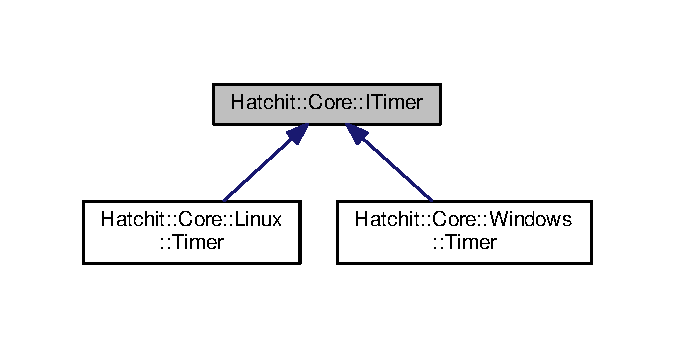
\includegraphics[width=324pt]{classHatchit_1_1Core_1_1ITimer__inherit__graph}
\end{center}
\end{figure}
\subsection*{Public Member Functions}
\begin{DoxyCompactItemize}
\item 
virtual void \hyperlink{classHatchit_1_1Core_1_1ITimer_abf16ebbb5a924fc20cf3099280f74cf7}{Start} ()=0
\begin{DoxyCompactList}\small\item\em Starts tracking time from moment this function is called. \end{DoxyCompactList}\item 
virtual void \hyperlink{classHatchit_1_1Core_1_1ITimer_a6969cb6203be6fd3d3a002146bb55fa1}{Tick} ()=0
\begin{DoxyCompactList}\small\item\em Calculates the delta time and total time. \end{DoxyCompactList}\item 
virtual void \hyperlink{classHatchit_1_1Core_1_1ITimer_a3bb9bec5874fd1c706ced3ba8033c761}{Stop} ()=0
\begin{DoxyCompactList}\small\item\em Stops timer. \end{DoxyCompactList}\item 
virtual void \hyperlink{classHatchit_1_1Core_1_1ITimer_a4f6fc1ec97ef9345d64e75bdeadcdad2}{Reset} ()=0
\begin{DoxyCompactList}\small\item\em Resets the timer data. \end{DoxyCompactList}\item 
virtual float \hyperlink{classHatchit_1_1Core_1_1ITimer_aef2f629b7e527640a62af97dad17dcb2}{Elapsed\+Time} () const =0
\begin{DoxyCompactList}\small\item\em Gets elapsed time (in seconds) \end{DoxyCompactList}\item 
virtual float \hyperlink{classHatchit_1_1Core_1_1ITimer_af5d9551ef9a0a98591f823b014efca11}{Total\+Time} () const =0
\begin{DoxyCompactList}\small\item\em Gets total time (in seconds) \end{DoxyCompactList}\item 
virtual float \hyperlink{classHatchit_1_1Core_1_1ITimer_a201d0dd1503b393ea7c1e1acfb402cd5}{Delta\+Time} () const =0
\begin{DoxyCompactList}\small\item\em Gets delta time (in seconds) \end{DoxyCompactList}\end{DoxyCompactItemize}
\subsection*{Protected Member Functions}
\begin{DoxyCompactItemize}
\item 
\hyperlink{classHatchit_1_1Core_1_1ITimer_a6e778117ed24325b99b3b5f258695bec}{I\+Timer} ()=default
\begin{DoxyCompactList}\small\item\em Creates instance of timer. \end{DoxyCompactList}\end{DoxyCompactItemize}


\subsection{Detailed Description}
Interface to describe timer functionality. 

Interface that describes the functionality of a timer. Used to link usability between a \hyperlink{namespaceWindows}{Windows} timer and a \hyperlink{namespaceLinux}{Linux} timer. 

Definition at line 41 of file ht\+\_\+timer.\+h.



\subsection{Constructor \& Destructor Documentation}
\index{Hatchit\+::\+Core\+::\+I\+Timer@{Hatchit\+::\+Core\+::\+I\+Timer}!I\+Timer@{I\+Timer}}
\index{I\+Timer@{I\+Timer}!Hatchit\+::\+Core\+::\+I\+Timer@{Hatchit\+::\+Core\+::\+I\+Timer}}
\subsubsection[{\texorpdfstring{I\+Timer()=default}{ITimer()=default}}]{\setlength{\rightskip}{0pt plus 5cm}Hatchit\+::\+Core\+::\+I\+Timer\+::\+I\+Timer (
\begin{DoxyParamCaption}
{}
\end{DoxyParamCaption}
)\hspace{0.3cm}{\ttfamily [protected]}, {\ttfamily [default]}}\hypertarget{classHatchit_1_1Core_1_1ITimer_a6e778117ed24325b99b3b5f258695bec}{}\label{classHatchit_1_1Core_1_1ITimer_a6e778117ed24325b99b3b5f258695bec}


Creates instance of timer. 

Created instance must then be started. 

\subsection{Member Function Documentation}
\index{Hatchit\+::\+Core\+::\+I\+Timer@{Hatchit\+::\+Core\+::\+I\+Timer}!Delta\+Time@{Delta\+Time}}
\index{Delta\+Time@{Delta\+Time}!Hatchit\+::\+Core\+::\+I\+Timer@{Hatchit\+::\+Core\+::\+I\+Timer}}
\subsubsection[{\texorpdfstring{Delta\+Time() const =0}{DeltaTime() const =0}}]{\setlength{\rightskip}{0pt plus 5cm}virtual float Hatchit\+::\+Core\+::\+I\+Timer\+::\+Delta\+Time (
\begin{DoxyParamCaption}
{}
\end{DoxyParamCaption}
) const\hspace{0.3cm}{\ttfamily [pure virtual]}}\hypertarget{classHatchit_1_1Core_1_1ITimer_a201d0dd1503b393ea7c1e1acfb402cd5}{}\label{classHatchit_1_1Core_1_1ITimer_a201d0dd1503b393ea7c1e1acfb402cd5}


Gets delta time (in seconds) 

Returns delta time (in seconds) between last two ticks of timer. 

Implemented in \hyperlink{classHatchit_1_1Core_1_1Linux_1_1Timer_aefd9ad0a2297d03e3877c0c6c900bd1c}{Hatchit\+::\+Core\+::\+Linux\+::\+Timer}, and \hyperlink{classHatchit_1_1Core_1_1Windows_1_1Timer_a79a80293593eb0d0785e896bbf7c934b}{Hatchit\+::\+Core\+::\+Windows\+::\+Timer}.

\index{Hatchit\+::\+Core\+::\+I\+Timer@{Hatchit\+::\+Core\+::\+I\+Timer}!Elapsed\+Time@{Elapsed\+Time}}
\index{Elapsed\+Time@{Elapsed\+Time}!Hatchit\+::\+Core\+::\+I\+Timer@{Hatchit\+::\+Core\+::\+I\+Timer}}
\subsubsection[{\texorpdfstring{Elapsed\+Time() const =0}{ElapsedTime() const =0}}]{\setlength{\rightskip}{0pt plus 5cm}virtual float Hatchit\+::\+Core\+::\+I\+Timer\+::\+Elapsed\+Time (
\begin{DoxyParamCaption}
{}
\end{DoxyParamCaption}
) const\hspace{0.3cm}{\ttfamily [pure virtual]}}\hypertarget{classHatchit_1_1Core_1_1ITimer_aef2f629b7e527640a62af97dad17dcb2}{}\label{classHatchit_1_1Core_1_1ITimer_aef2f629b7e527640a62af97dad17dcb2}


Gets elapsed time (in seconds) 

Returns elapsed time (in seconds) between \hyperlink{classHatchit_1_1Core_1_1ITimer_abf16ebbb5a924fc20cf3099280f74cf7}{Start()} and \hyperlink{classHatchit_1_1Core_1_1ITimer_a3bb9bec5874fd1c706ced3ba8033c761}{Stop()} calls. 

Implemented in \hyperlink{classHatchit_1_1Core_1_1Linux_1_1Timer_aa8e7a94df99e3953eebbb0d08d1dd8a2}{Hatchit\+::\+Core\+::\+Linux\+::\+Timer}, and \hyperlink{classHatchit_1_1Core_1_1Windows_1_1Timer_a4cda627adbe26e6f2b5438681063995e}{Hatchit\+::\+Core\+::\+Windows\+::\+Timer}.

\index{Hatchit\+::\+Core\+::\+I\+Timer@{Hatchit\+::\+Core\+::\+I\+Timer}!Reset@{Reset}}
\index{Reset@{Reset}!Hatchit\+::\+Core\+::\+I\+Timer@{Hatchit\+::\+Core\+::\+I\+Timer}}
\subsubsection[{\texorpdfstring{Reset()=0}{Reset()=0}}]{\setlength{\rightskip}{0pt plus 5cm}virtual void Hatchit\+::\+Core\+::\+I\+Timer\+::\+Reset (
\begin{DoxyParamCaption}
{}
\end{DoxyParamCaption}
)\hspace{0.3cm}{\ttfamily [pure virtual]}}\hypertarget{classHatchit_1_1Core_1_1ITimer_a4f6fc1ec97ef9345d64e75bdeadcdad2}{}\label{classHatchit_1_1Core_1_1ITimer_a4f6fc1ec97ef9345d64e75bdeadcdad2}


Resets the timer data. 

If timer is currently running, delta time will be calculated between the tick this function is called and the tick that \hyperlink{classHatchit_1_1Core_1_1ITimer_a6969cb6203be6fd3d3a002146bb55fa1}{Tick()} is called. 

Implemented in \hyperlink{classHatchit_1_1Core_1_1Linux_1_1Timer_a1159f074a5290718acee991decd80af3}{Hatchit\+::\+Core\+::\+Linux\+::\+Timer}, and \hyperlink{classHatchit_1_1Core_1_1Windows_1_1Timer_a464c6b3e3017867bd387a8fb477ad186}{Hatchit\+::\+Core\+::\+Windows\+::\+Timer}.

\index{Hatchit\+::\+Core\+::\+I\+Timer@{Hatchit\+::\+Core\+::\+I\+Timer}!Start@{Start}}
\index{Start@{Start}!Hatchit\+::\+Core\+::\+I\+Timer@{Hatchit\+::\+Core\+::\+I\+Timer}}
\subsubsection[{\texorpdfstring{Start()=0}{Start()=0}}]{\setlength{\rightskip}{0pt plus 5cm}virtual void Hatchit\+::\+Core\+::\+I\+Timer\+::\+Start (
\begin{DoxyParamCaption}
{}
\end{DoxyParamCaption}
)\hspace{0.3cm}{\ttfamily [pure virtual]}}\hypertarget{classHatchit_1_1Core_1_1ITimer_abf16ebbb5a924fc20cf3099280f74cf7}{}\label{classHatchit_1_1Core_1_1ITimer_abf16ebbb5a924fc20cf3099280f74cf7}


Starts tracking time from moment this function is called. 

Starts tracking time from moment this function is called. 

Implemented in \hyperlink{classHatchit_1_1Core_1_1Linux_1_1Timer_ad71a11915c848a40be11b2a2a1c24375}{Hatchit\+::\+Core\+::\+Linux\+::\+Timer}, and \hyperlink{classHatchit_1_1Core_1_1Windows_1_1Timer_a6441edbd90a09f4cfbca01fafd4d0aff}{Hatchit\+::\+Core\+::\+Windows\+::\+Timer}.

\index{Hatchit\+::\+Core\+::\+I\+Timer@{Hatchit\+::\+Core\+::\+I\+Timer}!Stop@{Stop}}
\index{Stop@{Stop}!Hatchit\+::\+Core\+::\+I\+Timer@{Hatchit\+::\+Core\+::\+I\+Timer}}
\subsubsection[{\texorpdfstring{Stop()=0}{Stop()=0}}]{\setlength{\rightskip}{0pt plus 5cm}virtual void Hatchit\+::\+Core\+::\+I\+Timer\+::\+Stop (
\begin{DoxyParamCaption}
{}
\end{DoxyParamCaption}
)\hspace{0.3cm}{\ttfamily [pure virtual]}}\hypertarget{classHatchit_1_1Core_1_1ITimer_a3bb9bec5874fd1c706ced3ba8033c761}{}\label{classHatchit_1_1Core_1_1ITimer_a3bb9bec5874fd1c706ced3ba8033c761}


Stops timer. 

Stops tracking timing information 

Implemented in \hyperlink{classHatchit_1_1Core_1_1Linux_1_1Timer_a93adf56776127d8c3215024f6566837b}{Hatchit\+::\+Core\+::\+Linux\+::\+Timer}, and \hyperlink{classHatchit_1_1Core_1_1Windows_1_1Timer_a1d9f06759a7a48e807d4b2a0254e7dbc}{Hatchit\+::\+Core\+::\+Windows\+::\+Timer}.

\index{Hatchit\+::\+Core\+::\+I\+Timer@{Hatchit\+::\+Core\+::\+I\+Timer}!Tick@{Tick}}
\index{Tick@{Tick}!Hatchit\+::\+Core\+::\+I\+Timer@{Hatchit\+::\+Core\+::\+I\+Timer}}
\subsubsection[{\texorpdfstring{Tick()=0}{Tick()=0}}]{\setlength{\rightskip}{0pt plus 5cm}virtual void Hatchit\+::\+Core\+::\+I\+Timer\+::\+Tick (
\begin{DoxyParamCaption}
{}
\end{DoxyParamCaption}
)\hspace{0.3cm}{\ttfamily [pure virtual]}}\hypertarget{classHatchit_1_1Core_1_1ITimer_a6969cb6203be6fd3d3a002146bb55fa1}{}\label{classHatchit_1_1Core_1_1ITimer_a6969cb6203be6fd3d3a002146bb55fa1}


Calculates the delta time and total time. 

Calculates the delta time between this tick and the last tick, or the last reset, depending on which happened more recently. Also recalculates the total time by accruing the calculated delta time into the total time. 

Implemented in \hyperlink{classHatchit_1_1Core_1_1Linux_1_1Timer_aafd5b502c0fda46aad2f38b47a6974d6}{Hatchit\+::\+Core\+::\+Linux\+::\+Timer}, and \hyperlink{classHatchit_1_1Core_1_1Windows_1_1Timer_ae1879dac284fc160b0322f5a57aa8ae3}{Hatchit\+::\+Core\+::\+Windows\+::\+Timer}.

\index{Hatchit\+::\+Core\+::\+I\+Timer@{Hatchit\+::\+Core\+::\+I\+Timer}!Total\+Time@{Total\+Time}}
\index{Total\+Time@{Total\+Time}!Hatchit\+::\+Core\+::\+I\+Timer@{Hatchit\+::\+Core\+::\+I\+Timer}}
\subsubsection[{\texorpdfstring{Total\+Time() const =0}{TotalTime() const =0}}]{\setlength{\rightskip}{0pt plus 5cm}virtual float Hatchit\+::\+Core\+::\+I\+Timer\+::\+Total\+Time (
\begin{DoxyParamCaption}
{}
\end{DoxyParamCaption}
) const\hspace{0.3cm}{\ttfamily [pure virtual]}}\hypertarget{classHatchit_1_1Core_1_1ITimer_af5d9551ef9a0a98591f823b014efca11}{}\label{classHatchit_1_1Core_1_1ITimer_af5d9551ef9a0a98591f823b014efca11}


Gets total time (in seconds) 

Returns total time between when timer was started and last tick. 

Implemented in \hyperlink{classHatchit_1_1Core_1_1Linux_1_1Timer_a9ca1371d09e3fd4ddb72ea4f6b9fb9d9}{Hatchit\+::\+Core\+::\+Linux\+::\+Timer}, and \hyperlink{classHatchit_1_1Core_1_1Windows_1_1Timer_a5cc4dcb2292ef3e12a5855990c296ab7}{Hatchit\+::\+Core\+::\+Windows\+::\+Timer}.



The documentation for this interface was generated from the following file\+:\begin{DoxyCompactItemize}
\item 
/home/debunez/\+Git\+Hub/\+Hatchit\+Editor/\+Hatchit/\+Hatchit\+Core/include/\hyperlink{ht__timer_8h}{ht\+\_\+timer.\+h}\end{DoxyCompactItemize}

\hypertarget{classHatchit_1_1Core_1_1Job}{}\section{Hatchit\+:\+:Core\+:\+:Job Class Reference}
\label{classHatchit_1_1Core_1_1Job}\index{Hatchit\+::\+Core\+::\+Job@{Hatchit\+::\+Core\+::\+Job}}


Describes a function to be threaded.  




{\ttfamily \#include $<$ht\+\_\+scheduler.\+h$>$}



Inheritance diagram for Hatchit\+:\+:Core\+:\+:Job\+:
\nopagebreak
\begin{figure}[H]
\begin{center}
\leavevmode
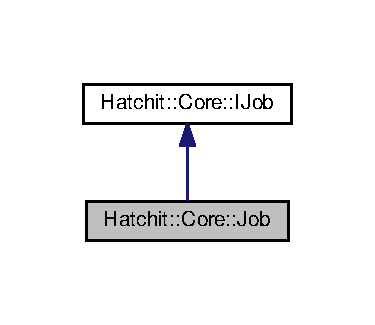
\includegraphics[width=180pt]{classHatchit_1_1Core_1_1Job__inherit__graph}
\end{center}
\end{figure}


Collaboration diagram for Hatchit\+:\+:Core\+:\+:Job\+:
\nopagebreak
\begin{figure}[H]
\begin{center}
\leavevmode
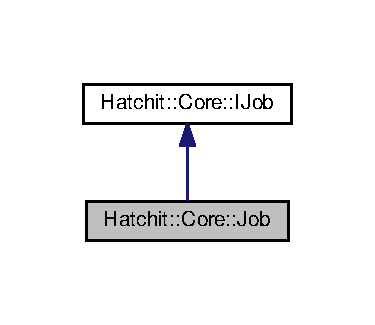
\includegraphics[width=180pt]{classHatchit_1_1Core_1_1Job__coll__graph}
\end{center}
\end{figure}
\subsection*{Public Member Functions}
\begin{DoxyCompactItemize}
\item 
{\bfseries Job} (std\+::function$<$ void()$>$ function)\hypertarget{classHatchit_1_1Core_1_1Job_a7b39934793bb408dfa2e7dc536326ae1}{}\label{classHatchit_1_1Core_1_1Job_a7b39934793bb408dfa2e7dc536326ae1}

\item 
std\+::thread {\bfseries Get\+Thread} () override\hypertarget{classHatchit_1_1Core_1_1Job_ab4edf2e76e836f3a3690dc01f69f7a88}{}\label{classHatchit_1_1Core_1_1Job_ab4edf2e76e836f3a3690dc01f69f7a88}

\end{DoxyCompactItemize}


\subsection{Detailed Description}
Describes a function to be threaded. 

Definition at line 56 of file ht\+\_\+scheduler.\+h.



The documentation for this class was generated from the following file\+:\begin{DoxyCompactItemize}
\item 
/home/debunez/\+Git\+Hub/\+Hatchit\+Editor/\+Hatchit/\+Hatchit\+Core/include/ht\+\_\+scheduler.\+h\end{DoxyCompactItemize}

\hypertarget{classHatchit_1_1Core_1_1Profiler}{}\section{Hatchit\+:\+:Core\+:\+:Profiler Class Reference}
\label{classHatchit_1_1Core_1_1Profiler}\index{Hatchit\+::\+Core\+::\+Profiler@{Hatchit\+::\+Core\+::\+Profiler}}


Defines a Runtime \hyperlink{classHatchit_1_1Core_1_1Profiler}{Profiler} \hyperlink{classHatchit_1_1Core_1_1Singleton}{Singleton}.  




{\ttfamily \#include $<$ht\+\_\+profiler.\+h$>$}



Inheritance diagram for Hatchit\+:\+:Core\+:\+:Profiler\+:
\nopagebreak
\begin{figure}[H]
\begin{center}
\leavevmode
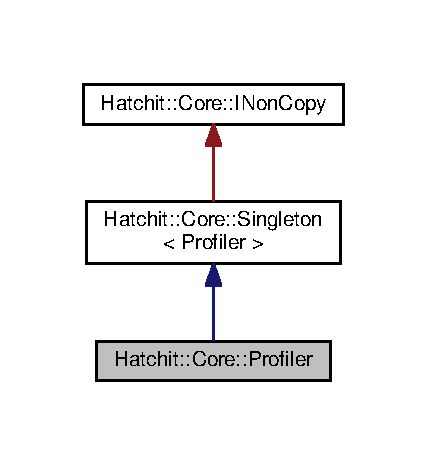
\includegraphics[width=205pt]{classHatchit_1_1Core_1_1Profiler__inherit__graph}
\end{center}
\end{figure}


Collaboration diagram for Hatchit\+:\+:Core\+:\+:Profiler\+:
\nopagebreak
\begin{figure}[H]
\begin{center}
\leavevmode
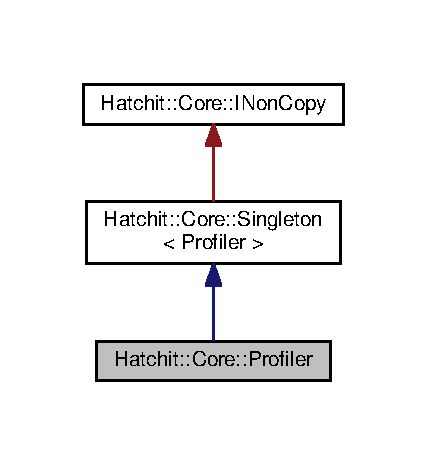
\includegraphics[width=205pt]{classHatchit_1_1Core_1_1Profiler__coll__graph}
\end{center}
\end{figure}
\subsection*{Classes}
\begin{DoxyCompactItemize}
\item 
class \hyperlink{classHatchit_1_1Core_1_1Profiler_1_1Sample}{Sample}
\end{DoxyCompactItemize}
\subsection*{Static Public Member Functions}
\begin{DoxyCompactItemize}
\item 
static void {\bfseries Push\+Sample} (\hyperlink{classHatchit_1_1Core_1_1Profiler_1_1Sample}{Sample} $\ast$sample)\hypertarget{classHatchit_1_1Core_1_1Profiler_a0f8f9eb4507261bef45527995e6a3c19}{}\label{classHatchit_1_1Core_1_1Profiler_a0f8f9eb4507261bef45527995e6a3c19}

\item 
static void {\bfseries Pop\+Sample} ()\hypertarget{classHatchit_1_1Core_1_1Profiler_af693980d00fc01b6d379ec1b3019b37b}{}\label{classHatchit_1_1Core_1_1Profiler_af693980d00fc01b6d379ec1b3019b37b}

\item 
static void {\bfseries Dump} ()\hypertarget{classHatchit_1_1Core_1_1Profiler_af88668910468a12f2aa7383ea444d14c}{}\label{classHatchit_1_1Core_1_1Profiler_af88668910468a12f2aa7383ea444d14c}

\end{DoxyCompactItemize}


\subsection{Detailed Description}
Defines a Runtime \hyperlink{classHatchit_1_1Core_1_1Profiler}{Profiler} \hyperlink{classHatchit_1_1Core_1_1Singleton}{Singleton}. 

This runtime profiler singleton manages all runtime profiling samples and managers the distributiion and hierarchy of the samples

N\+O\+TE\+: The current implementation does not support distributed hierarchical sampling. 

Definition at line 42 of file ht\+\_\+profiler.\+h.



The documentation for this class was generated from the following file\+:\begin{DoxyCompactItemize}
\item 
/home/debunez/\+Git\+Hub/\+Hatchit\+Editor/\+Hatchit/\+Hatchit\+Core/include/ht\+\_\+profiler.\+h\end{DoxyCompactItemize}

\hypertarget{classHatchit_1_1Core_1_1Profiler_1_1Sample}{}\section{Hatchit\+:\+:Core\+:\+:Profiler\+:\+:Sample Class Reference}
\label{classHatchit_1_1Core_1_1Profiler_1_1Sample}\index{Hatchit\+::\+Core\+::\+Profiler\+::\+Sample@{Hatchit\+::\+Core\+::\+Profiler\+::\+Sample}}
\subsection*{Public Member Functions}
\begin{DoxyCompactItemize}
\item 
{\bfseries Sample} (const std\+::string \&name, float elapsed\+Time)\hypertarget{classHatchit_1_1Core_1_1Profiler_1_1Sample_a3c80272e5292fa8ee0ba6e90554ab345}{}\label{classHatchit_1_1Core_1_1Profiler_1_1Sample_a3c80272e5292fa8ee0ba6e90554ab345}

\item 
const std\+::string \& {\bfseries Name} () const \hypertarget{classHatchit_1_1Core_1_1Profiler_1_1Sample_a710a121cbc0bbf8d4eb69ac4adb30f2c}{}\label{classHatchit_1_1Core_1_1Profiler_1_1Sample_a710a121cbc0bbf8d4eb69ac4adb30f2c}

\item 
const uint32\+\_\+t {\bfseries Count} () const \hypertarget{classHatchit_1_1Core_1_1Profiler_1_1Sample_a6cbf8edc2552fa40f274757c5fea032c}{}\label{classHatchit_1_1Core_1_1Profiler_1_1Sample_a6cbf8edc2552fa40f274757c5fea032c}

\item 
const float {\bfseries Elapsed\+Time} () const \hypertarget{classHatchit_1_1Core_1_1Profiler_1_1Sample_a9cd0c7b742fe350de1132601b86e8a16}{}\label{classHatchit_1_1Core_1_1Profiler_1_1Sample_a9cd0c7b742fe350de1132601b86e8a16}

\item 
void {\bfseries Set\+Name} (const std\+::string \&name)\hypertarget{classHatchit_1_1Core_1_1Profiler_1_1Sample_a591f8e3a9594e4334836b2eef8e00603}{}\label{classHatchit_1_1Core_1_1Profiler_1_1Sample_a591f8e3a9594e4334836b2eef8e00603}

\item 
void {\bfseries Set\+Count} (uint32\+\_\+t count)\hypertarget{classHatchit_1_1Core_1_1Profiler_1_1Sample_a2c3f58cfddabb2bf3d55f1abaee6b1f9}{}\label{classHatchit_1_1Core_1_1Profiler_1_1Sample_a2c3f58cfddabb2bf3d55f1abaee6b1f9}

\item 
void {\bfseries Set\+Elapsed\+Time} (float elapsed)\hypertarget{classHatchit_1_1Core_1_1Profiler_1_1Sample_a6147e57591cddf7a0d3ef5840985a225}{}\label{classHatchit_1_1Core_1_1Profiler_1_1Sample_a6147e57591cddf7a0d3ef5840985a225}

\item 
void {\bfseries Increment} ()\hypertarget{classHatchit_1_1Core_1_1Profiler_1_1Sample_a2130172aa15536fd73b70d9e47f6346a}{}\label{classHatchit_1_1Core_1_1Profiler_1_1Sample_a2130172aa15536fd73b70d9e47f6346a}

\item 
void {\bfseries Decrement} ()\hypertarget{classHatchit_1_1Core_1_1Profiler_1_1Sample_aa5f5db9feca34cc338440554ca1234a3}{}\label{classHatchit_1_1Core_1_1Profiler_1_1Sample_aa5f5db9feca34cc338440554ca1234a3}

\item 
void {\bfseries Add\+Child} (\hyperlink{classHatchit_1_1Core_1_1Profiler_1_1Sample}{Sample} \&child)\hypertarget{classHatchit_1_1Core_1_1Profiler_1_1Sample_ad638b416c1d512383a2f5cc53531200b}{}\label{classHatchit_1_1Core_1_1Profiler_1_1Sample_ad638b416c1d512383a2f5cc53531200b}

\item 
const std\+::vector$<$ \hyperlink{classHatchit_1_1Core_1_1Profiler_1_1Sample}{Sample} $>$ \& {\bfseries Children} ()\hypertarget{classHatchit_1_1Core_1_1Profiler_1_1Sample_acae871ed9cac913f3b2c117c5c6f6fdb}{}\label{classHatchit_1_1Core_1_1Profiler_1_1Sample_acae871ed9cac913f3b2c117c5c6f6fdb}

\end{DoxyCompactItemize}


\subsection{Detailed Description}


Definition at line 45 of file ht\+\_\+profiler.\+h.



The documentation for this class was generated from the following file\+:\begin{DoxyCompactItemize}
\item 
/home/debunez/\+Git\+Hub/\+Hatchit\+Editor/\+Hatchit/\+Hatchit\+Core/include/ht\+\_\+profiler.\+h\end{DoxyCompactItemize}

\hypertarget{classHatchit_1_1Core_1_1Scheduler}{}\section{Hatchit\+:\+:Core\+:\+:Scheduler Class Reference}
\label{classHatchit_1_1Core_1_1Scheduler}\index{Hatchit\+::\+Core\+::\+Scheduler@{Hatchit\+::\+Core\+::\+Scheduler}}


A manager that schedules and submits jobs to threads as they are available.  




{\ttfamily \#include $<$ht\+\_\+scheduler.\+h$>$}



Inheritance diagram for Hatchit\+:\+:Core\+:\+:Scheduler\+:
\nopagebreak
\begin{figure}[H]
\begin{center}
\leavevmode
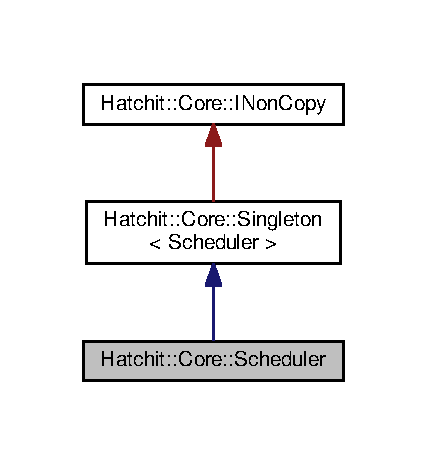
\includegraphics[width=205pt]{classHatchit_1_1Core_1_1Scheduler__inherit__graph}
\end{center}
\end{figure}


Collaboration diagram for Hatchit\+:\+:Core\+:\+:Scheduler\+:
\nopagebreak
\begin{figure}[H]
\begin{center}
\leavevmode
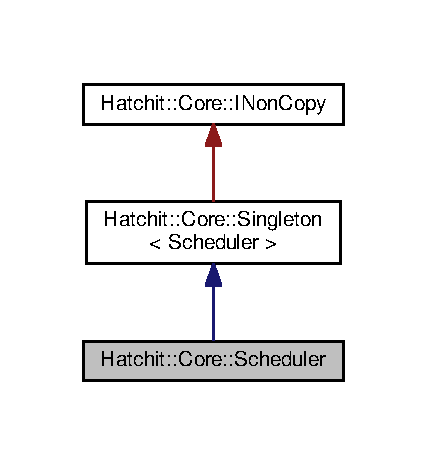
\includegraphics[width=205pt]{classHatchit_1_1Core_1_1Scheduler__coll__graph}
\end{center}
\end{figure}
\subsection*{Static Public Member Functions}
\begin{DoxyCompactItemize}
\item 
static void {\bfseries Initialize} ()\hypertarget{classHatchit_1_1Core_1_1Scheduler_aaaa1302b7bbc52e75bc4c23b8d6f016a}{}\label{classHatchit_1_1Core_1_1Scheduler_aaaa1302b7bbc52e75bc4c23b8d6f016a}

\item 
{\footnotesize template$<$class Func , class... Args$>$ }\\static void {\bfseries Schedule\+Job} (Func \&\&function, Args \&\&...arguments)\hypertarget{classHatchit_1_1Core_1_1Scheduler_a078c9f11edc0ab0f1b595e9298374d6f}{}\label{classHatchit_1_1Core_1_1Scheduler_a078c9f11edc0ab0f1b595e9298374d6f}

\item 
static void {\bfseries Run\+Jobs} ()\hypertarget{classHatchit_1_1Core_1_1Scheduler_a47863a38c261d59ae9b5e91d2ba521fd}{}\label{classHatchit_1_1Core_1_1Scheduler_a47863a38c261d59ae9b5e91d2ba521fd}

\end{DoxyCompactItemize}


\subsection{Detailed Description}
A manager that schedules and submits jobs to threads as they are available. 

Supply this manager with function pointers (jobs) and it should schedule and sync these jobs appropriately across however many threads are on the hardware. 

Definition at line 76 of file ht\+\_\+scheduler.\+h.



The documentation for this class was generated from the following file\+:\begin{DoxyCompactItemize}
\item 
/home/debunez/\+Git\+Hub/\+Hatchit\+Editor/\+Hatchit/\+Hatchit\+Core/include/ht\+\_\+scheduler.\+h\end{DoxyCompactItemize}

\hypertarget{classHatchit_1_1Core_1_1ScopedThread}{}\section{Hatchit\+:\+:Core\+:\+:Scoped\+Thread Class Reference}
\label{classHatchit_1_1Core_1_1ScopedThread}\index{Hatchit\+::\+Core\+::\+Scoped\+Thread@{Hatchit\+::\+Core\+::\+Scoped\+Thread}}


A safety wrapper for std\+::threads to safely join threads.  




{\ttfamily \#include $<$ht\+\_\+scopedthread.\+h$>$}



Inheritance diagram for Hatchit\+:\+:Core\+:\+:Scoped\+Thread\+:
\nopagebreak
\begin{figure}[H]
\begin{center}
\leavevmode
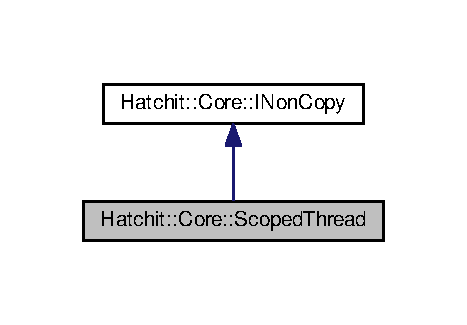
\includegraphics[width=224pt]{classHatchit_1_1Core_1_1ScopedThread__inherit__graph}
\end{center}
\end{figure}


Collaboration diagram for Hatchit\+:\+:Core\+:\+:Scoped\+Thread\+:
\nopagebreak
\begin{figure}[H]
\begin{center}
\leavevmode
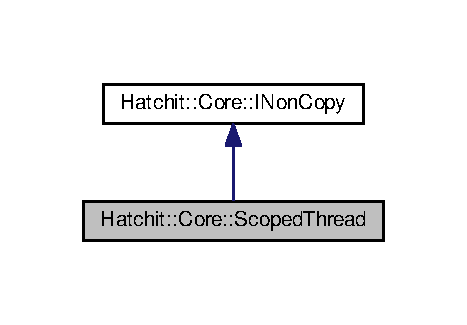
\includegraphics[width=224pt]{classHatchit_1_1Core_1_1ScopedThread__coll__graph}
\end{center}
\end{figure}
\subsection*{Public Member Functions}
\begin{DoxyCompactItemize}
\item 
{\bfseries Scoped\+Thread} (std\+::thread \+\_\+t)\hypertarget{classHatchit_1_1Core_1_1ScopedThread_aee8330560a7636968f8d0d3ffe991622}{}\label{classHatchit_1_1Core_1_1ScopedThread_aee8330560a7636968f8d0d3ffe991622}

\end{DoxyCompactItemize}
\subsection*{Additional Inherited Members}


\subsection{Detailed Description}
A safety wrapper for std\+::threads to safely join threads. 

Definition at line 30 of file ht\+\_\+scopedthread.\+h.



The documentation for this class was generated from the following file\+:\begin{DoxyCompactItemize}
\item 
/home/debunez/\+Git\+Hub/\+Hatchit\+Editor/\+Hatchit/\+Hatchit\+Core/include/ht\+\_\+scopedthread.\+h\end{DoxyCompactItemize}

\hypertarget{classHatchit_1_1Core_1_1Singleton}{}\section{Hatchit\+:\+:Core\+:\+:Singleton$<$ T $>$ Class Template Reference}
\label{classHatchit_1_1Core_1_1Singleton}\index{Hatchit\+::\+Core\+::\+Singleton$<$ T $>$@{Hatchit\+::\+Core\+::\+Singleton$<$ T $>$}}


Describes class that has only one instance avialable globally.  




{\ttfamily \#include $<$ht\+\_\+singleton.\+h$>$}



Inheritance diagram for Hatchit\+:\+:Core\+:\+:Singleton$<$ T $>$\+:
\nopagebreak
\begin{figure}[H]
\begin{center}
\leavevmode
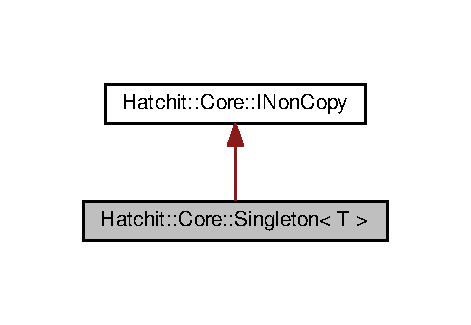
\includegraphics[width=226pt]{classHatchit_1_1Core_1_1Singleton__inherit__graph}
\end{center}
\end{figure}


Collaboration diagram for Hatchit\+:\+:Core\+:\+:Singleton$<$ T $>$\+:
\nopagebreak
\begin{figure}[H]
\begin{center}
\leavevmode
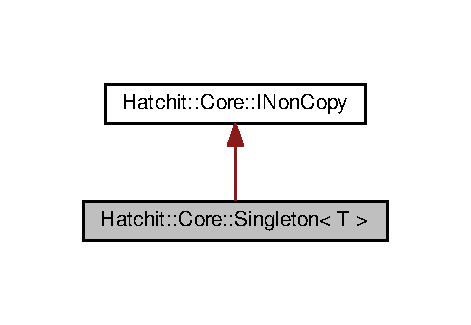
\includegraphics[width=226pt]{classHatchit_1_1Core_1_1Singleton__coll__graph}
\end{center}
\end{figure}
\subsection*{Static Public Member Functions}
\begin{DoxyCompactItemize}
\item 
static T \& \hyperlink{classHatchit_1_1Core_1_1Singleton_a43b6d0ea72ff1cab8a6868aeee1ba43b}{instance} ()
\begin{DoxyCompactList}\small\item\em Provides reference to single instance of class. \end{DoxyCompactList}\end{DoxyCompactItemize}


\subsection{Detailed Description}
\subsubsection*{template$<$typename T$>$\\*
class Hatchit\+::\+Core\+::\+Singleton$<$ T $>$}

Describes class that has only one instance avialable globally. 

Describes class that has only one instance available globally. Is unable to be copied or instantiated elsewhere. 

Definition at line 43 of file ht\+\_\+singleton.\+h.



\subsection{Member Function Documentation}
\index{Hatchit\+::\+Core\+::\+Singleton@{Hatchit\+::\+Core\+::\+Singleton}!instance@{instance}}
\index{instance@{instance}!Hatchit\+::\+Core\+::\+Singleton@{Hatchit\+::\+Core\+::\+Singleton}}
\subsubsection[{\texorpdfstring{instance()}{instance()}}]{\setlength{\rightskip}{0pt plus 5cm}template$<$typename T$>$ static T\& {\bf Hatchit\+::\+Core\+::\+Singleton}$<$ T $>$\+::instance (
\begin{DoxyParamCaption}
{}
\end{DoxyParamCaption}
)\hspace{0.3cm}{\ttfamily [static]}}\hypertarget{classHatchit_1_1Core_1_1Singleton_a43b6d0ea72ff1cab8a6868aeee1ba43b}{}\label{classHatchit_1_1Core_1_1Singleton_a43b6d0ea72ff1cab8a6868aeee1ba43b}


Provides reference to single instance of class. 

Provides mutable reference to single instance of singleton class. 

The documentation for this class was generated from the following file\+:\begin{DoxyCompactItemize}
\item 
/home/debunez/\+Git\+Hub/\+Hatchit\+Editor/\+Hatchit/\+Hatchit\+Core/include/\hyperlink{ht__singleton_8h}{ht\+\_\+singleton.\+h}\end{DoxyCompactItemize}

\hypertarget{classHatchit_1_1Core_1_1ThreadsafeQueue}{}\section{Hatchit\+:\+:Core\+:\+:Threadsafe\+Queue$<$ T $>$ Class Template Reference}
\label{classHatchit_1_1Core_1_1ThreadsafeQueue}\index{Hatchit\+::\+Core\+::\+Threadsafe\+Queue$<$ T $>$@{Hatchit\+::\+Core\+::\+Threadsafe\+Queue$<$ T $>$}}
\subsection*{Public Member Functions}
\begin{DoxyCompactItemize}
\item 
{\bfseries Threadsafe\+Queue} (const \hyperlink{classHatchit_1_1Core_1_1ThreadsafeQueue}{Threadsafe\+Queue} \&other)\hypertarget{classHatchit_1_1Core_1_1ThreadsafeQueue_af1e902e4e4ea6f634936534fb6ef269e}{}\label{classHatchit_1_1Core_1_1ThreadsafeQueue_af1e902e4e4ea6f634936534fb6ef269e}

\item 
{\bfseries Threadsafe\+Queue} (\hyperlink{classHatchit_1_1Core_1_1ThreadsafeQueue}{Threadsafe\+Queue} \&\&other)\hypertarget{classHatchit_1_1Core_1_1ThreadsafeQueue_ac745ffa3f95c156b65c963e2e1250748}{}\label{classHatchit_1_1Core_1_1ThreadsafeQueue_ac745ffa3f95c156b65c963e2e1250748}

\item 
\hyperlink{classHatchit_1_1Core_1_1ThreadsafeQueue}{Threadsafe\+Queue} \& {\bfseries operator=} (const \hyperlink{classHatchit_1_1Core_1_1ThreadsafeQueue}{Threadsafe\+Queue} \&other)\hypertarget{classHatchit_1_1Core_1_1ThreadsafeQueue_aaa1c293954a66c135f946a80021fccbe}{}\label{classHatchit_1_1Core_1_1ThreadsafeQueue_aaa1c293954a66c135f946a80021fccbe}

\item 
\hyperlink{classHatchit_1_1Core_1_1ThreadsafeQueue}{Threadsafe\+Queue} \& {\bfseries operator=} (\hyperlink{classHatchit_1_1Core_1_1ThreadsafeQueue}{Threadsafe\+Queue} \&\&other)\hypertarget{classHatchit_1_1Core_1_1ThreadsafeQueue_a4e219499991f032fea0126adad1eb32d}{}\label{classHatchit_1_1Core_1_1ThreadsafeQueue_a4e219499991f032fea0126adad1eb32d}

\item 
void {\bfseries push} (T \+\_\+val)\hypertarget{classHatchit_1_1Core_1_1ThreadsafeQueue_a9f69e3e85d1a844b6928e7071a91d200}{}\label{classHatchit_1_1Core_1_1ThreadsafeQueue_a9f69e3e85d1a844b6928e7071a91d200}

\item 
std\+::shared\+\_\+ptr$<$ T $>$ {\bfseries wait\+\_\+pop} ()\hypertarget{classHatchit_1_1Core_1_1ThreadsafeQueue_a50081612b96914987affc028933e7063}{}\label{classHatchit_1_1Core_1_1ThreadsafeQueue_a50081612b96914987affc028933e7063}

\item 
void {\bfseries wait\+\_\+pop} (T \&out)\hypertarget{classHatchit_1_1Core_1_1ThreadsafeQueue_aa85536716c46b367e849b0129a75c9a8}{}\label{classHatchit_1_1Core_1_1ThreadsafeQueue_aa85536716c46b367e849b0129a75c9a8}

\item 
bool {\bfseries empty} () const \hypertarget{classHatchit_1_1Core_1_1ThreadsafeQueue_a16a953cf3da09bb6165c916aa3adca7d}{}\label{classHatchit_1_1Core_1_1ThreadsafeQueue_a16a953cf3da09bb6165c916aa3adca7d}

\end{DoxyCompactItemize}


\subsection{Detailed Description}
\subsubsection*{template$<$typename T$>$\\*
class Hatchit\+::\+Core\+::\+Threadsafe\+Queue$<$ T $>$}



Definition at line 35 of file ht\+\_\+threadqueue.\+h.



The documentation for this class was generated from the following file\+:\begin{DoxyCompactItemize}
\item 
/home/debunez/\+Git\+Hub/\+Hatchit\+Editor/\+Hatchit/\+Hatchit\+Core/include/ht\+\_\+threadqueue.\+h\end{DoxyCompactItemize}

\hypertarget{classThreadsafeQueue_3_01T_01_4}{}\section{Threadsafe\+Queue$<$ T $>$ Class Reference}
\label{classThreadsafeQueue_3_01T_01_4}\index{Threadsafe\+Queue$<$ T $>$@{Threadsafe\+Queue$<$ T $>$}}


wrapper for std\+::queue that provides thread-\/safe functions  




{\ttfamily \#include $<$ht\+\_\+threadqueue.\+h$>$}



\subsection{Detailed Description}
wrapper for std\+::queue that provides thread-\/safe functions 

The documentation for this class was generated from the following file\+:\begin{DoxyCompactItemize}
\item 
/home/debunez/\+Git\+Hub/\+Hatchit\+Editor/\+Hatchit/\+Hatchit\+Core/include/ht\+\_\+threadqueue.\+h\end{DoxyCompactItemize}

\hypertarget{classHatchit_1_1Core_1_1ThreadsafeStack}{}\section{Hatchit\+:\+:Core\+:\+:Threadsafe\+Stack$<$ T $>$ Class Template Reference}
\label{classHatchit_1_1Core_1_1ThreadsafeStack}\index{Hatchit\+::\+Core\+::\+Threadsafe\+Stack$<$ T $>$@{Hatchit\+::\+Core\+::\+Threadsafe\+Stack$<$ T $>$}}
\subsection*{Public Member Functions}
\begin{DoxyCompactItemize}
\item 
{\bfseries Threadsafe\+Stack} (const \hyperlink{classHatchit_1_1Core_1_1ThreadsafeStack}{Threadsafe\+Stack} \&other)\hypertarget{classHatchit_1_1Core_1_1ThreadsafeStack_a5c1e235499e48df8ae7b8568d9c0e5db}{}\label{classHatchit_1_1Core_1_1ThreadsafeStack_a5c1e235499e48df8ae7b8568d9c0e5db}

\item 
{\bfseries Threadsafe\+Stack} (\hyperlink{classHatchit_1_1Core_1_1ThreadsafeStack}{Threadsafe\+Stack} \&\&other)\hypertarget{classHatchit_1_1Core_1_1ThreadsafeStack_ae0ae8128839367b9d320b59d5396c037}{}\label{classHatchit_1_1Core_1_1ThreadsafeStack_ae0ae8128839367b9d320b59d5396c037}

\item 
\hyperlink{classHatchit_1_1Core_1_1ThreadsafeStack}{Threadsafe\+Stack} \& {\bfseries operator=} (const \hyperlink{classHatchit_1_1Core_1_1ThreadsafeStack}{Threadsafe\+Stack} \&)\hypertarget{classHatchit_1_1Core_1_1ThreadsafeStack_a5b86067376dc2a1b1ffad3ac4793a7da}{}\label{classHatchit_1_1Core_1_1ThreadsafeStack_a5b86067376dc2a1b1ffad3ac4793a7da}

\item 
\hyperlink{classHatchit_1_1Core_1_1ThreadsafeStack}{Threadsafe\+Stack} \& {\bfseries operator=} (\hyperlink{classHatchit_1_1Core_1_1ThreadsafeStack}{Threadsafe\+Stack} \&\&)\hypertarget{classHatchit_1_1Core_1_1ThreadsafeStack_a3a9220aa5dfa4ca704957beab9cd7d0d}{}\label{classHatchit_1_1Core_1_1ThreadsafeStack_a3a9220aa5dfa4ca704957beab9cd7d0d}

\item 
void {\bfseries push} (T \+\_\+val)\hypertarget{classHatchit_1_1Core_1_1ThreadsafeStack_a167c1fb0a36da427551d8f0e0ed62e7d}{}\label{classHatchit_1_1Core_1_1ThreadsafeStack_a167c1fb0a36da427551d8f0e0ed62e7d}

\item 
std\+::shared\+\_\+ptr$<$ T $>$ {\bfseries pop} ()\hypertarget{classHatchit_1_1Core_1_1ThreadsafeStack_aafae0641050816de8ca7c5090ab0a627}{}\label{classHatchit_1_1Core_1_1ThreadsafeStack_aafae0641050816de8ca7c5090ab0a627}

\item 
void {\bfseries pop} (T \&\+\_\+val)\hypertarget{classHatchit_1_1Core_1_1ThreadsafeStack_a4f6199d86eb2f311c9c58b3e23ad840e}{}\label{classHatchit_1_1Core_1_1ThreadsafeStack_a4f6199d86eb2f311c9c58b3e23ad840e}

\item 
bool {\bfseries empty} () const \hypertarget{classHatchit_1_1Core_1_1ThreadsafeStack_a9ac7b4af62073685e7150081003fd01c}{}\label{classHatchit_1_1Core_1_1ThreadsafeStack_a9ac7b4af62073685e7150081003fd01c}

\end{DoxyCompactItemize}


\subsection{Detailed Description}
\subsubsection*{template$<$typename T$>$\\*
class Hatchit\+::\+Core\+::\+Threadsafe\+Stack$<$ T $>$}



Definition at line 36 of file ht\+\_\+threadstack.\+h.



The documentation for this class was generated from the following file\+:\begin{DoxyCompactItemize}
\item 
/home/debunez/\+Git\+Hub/\+Hatchit\+Editor/\+Hatchit/\+Hatchit\+Core/include/ht\+\_\+threadstack.\+h\end{DoxyCompactItemize}

\hypertarget{classThreadsafeStack_3_01T_01_4}{}\section{Threadsafe\+Stack$<$ T $>$ Class Reference}
\label{classThreadsafeStack_3_01T_01_4}\index{Threadsafe\+Stack$<$ T $>$@{Threadsafe\+Stack$<$ T $>$}}


wrapper for std\+::stack that provides thread-\/safe functions  




{\ttfamily \#include $<$ht\+\_\+threadstack.\+h$>$}



\subsection{Detailed Description}
wrapper for std\+::stack that provides thread-\/safe functions 

The documentation for this class was generated from the following file\+:\begin{DoxyCompactItemize}
\item 
/home/debunez/\+Git\+Hub/\+Hatchit\+Editor/\+Hatchit/\+Hatchit\+Core/include/ht\+\_\+threadstack.\+h\end{DoxyCompactItemize}

\hypertarget{classHatchit_1_1Core_1_1ThreadsafeVector}{}\section{Hatchit\+:\+:Core\+:\+:Threadsafe\+Vector$<$ T $>$ Class Template Reference}
\label{classHatchit_1_1Core_1_1ThreadsafeVector}\index{Hatchit\+::\+Core\+::\+Threadsafe\+Vector$<$ T $>$@{Hatchit\+::\+Core\+::\+Threadsafe\+Vector$<$ T $>$}}


wrapper for std\+::vector that provides thread-\/safe functions  




{\ttfamily \#include $<$ht\+\_\+threadvector.\+h$>$}

\subsection*{Public Member Functions}
\begin{DoxyCompactItemize}
\item 
\hyperlink{classHatchit_1_1Core_1_1ThreadsafeVector_a458aa8190cfe60bd8b8a708f608a7232}{Threadsafe\+Vector} ()\hypertarget{classHatchit_1_1Core_1_1ThreadsafeVector_a458aa8190cfe60bd8b8a708f608a7232}{}\label{classHatchit_1_1Core_1_1ThreadsafeVector_a458aa8190cfe60bd8b8a708f608a7232}

\begin{DoxyCompactList}\small\item\em Creates empty \hyperlink{classHatchit_1_1Core_1_1ThreadsafeVector}{Threadsafe\+Vector}. \end{DoxyCompactList}\item 
\hyperlink{classHatchit_1_1Core_1_1ThreadsafeVector_abb29a6533d9e929a1e05a38118f2a789}{Threadsafe\+Vector} (const \hyperlink{classHatchit_1_1Core_1_1ThreadsafeVector}{Threadsafe\+Vector} \&other)\hypertarget{classHatchit_1_1Core_1_1ThreadsafeVector_abb29a6533d9e929a1e05a38118f2a789}{}\label{classHatchit_1_1Core_1_1ThreadsafeVector_abb29a6533d9e929a1e05a38118f2a789}

\begin{DoxyCompactList}\small\item\em Creates copy of given \hyperlink{classHatchit_1_1Core_1_1ThreadsafeVector}{Threadsafe\+Vector}. \end{DoxyCompactList}\item 
\hyperlink{classHatchit_1_1Core_1_1ThreadsafeVector_a855472c436c5df4dcaca0034b4466e44}{Threadsafe\+Vector} (\hyperlink{classHatchit_1_1Core_1_1ThreadsafeVector}{Threadsafe\+Vector} \&\&other)\hypertarget{classHatchit_1_1Core_1_1ThreadsafeVector_a855472c436c5df4dcaca0034b4466e44}{}\label{classHatchit_1_1Core_1_1ThreadsafeVector_a855472c436c5df4dcaca0034b4466e44}

\begin{DoxyCompactList}\small\item\em Moves data from given \hyperlink{classHatchit_1_1Core_1_1ThreadsafeVector}{Threadsafe\+Vector} into new \hyperlink{classHatchit_1_1Core_1_1ThreadsafeVector}{Threadsafe\+Vector}. \end{DoxyCompactList}\item 
\hyperlink{classHatchit_1_1Core_1_1ThreadsafeVector}{Threadsafe\+Vector} \& \hyperlink{classHatchit_1_1Core_1_1ThreadsafeVector_a0aa4b89e8f6b3f9472a7e5415e5d79b1}{operator=} (const \hyperlink{classHatchit_1_1Core_1_1ThreadsafeVector}{Threadsafe\+Vector} \&other)
\begin{DoxyCompactList}\small\item\em Copies data from one \hyperlink{classHatchit_1_1Core_1_1ThreadsafeVector}{Threadsafe\+Vector} into current \hyperlink{classHatchit_1_1Core_1_1ThreadsafeVector}{Threadsafe\+Vector}. \end{DoxyCompactList}\item 
\hyperlink{classHatchit_1_1Core_1_1ThreadsafeVector}{Threadsafe\+Vector} \& \hyperlink{classHatchit_1_1Core_1_1ThreadsafeVector_a8304a6dfe56e1af8e4ae6598d9250316}{operator=} (\hyperlink{classHatchit_1_1Core_1_1ThreadsafeVector}{Threadsafe\+Vector} \&\&other)
\begin{DoxyCompactList}\small\item\em Moves data from temporary \hyperlink{classHatchit_1_1Core_1_1ThreadsafeVector}{Threadsafe\+Vector} into current \hyperlink{classHatchit_1_1Core_1_1ThreadsafeVector}{Threadsafe\+Vector}. \end{DoxyCompactList}\item 
std\+::shared\+\_\+ptr$<$ T $>$ \hyperlink{classHatchit_1_1Core_1_1ThreadsafeVector_af1b460bf351cd2b73fa442a1fcce22cc}{operator\mbox{[}$\,$\mbox{]}} (size\+\_\+t pos)
\begin{DoxyCompactList}\small\item\em Returns a shared ptr copy to the element at specified location. \end{DoxyCompactList}\item 
void \hyperlink{classHatchit_1_1Core_1_1ThreadsafeVector_a8ca2359c9f28554e298d034e47ab84f9}{push\+\_\+back} (T \+\_\+val)\hypertarget{classHatchit_1_1Core_1_1ThreadsafeVector_a8ca2359c9f28554e298d034e47ab84f9}{}\label{classHatchit_1_1Core_1_1ThreadsafeVector_a8ca2359c9f28554e298d034e47ab84f9}

\begin{DoxyCompactList}\small\item\em Adds a new value to \hyperlink{classHatchit_1_1Core_1_1ThreadsafeVector}{Threadsafe\+Vector}. \end{DoxyCompactList}\item 
size\+\_\+t \hyperlink{classHatchit_1_1Core_1_1ThreadsafeVector_a262f6ae1582a59545c0f604983f4aa0f}{size} () const \hypertarget{classHatchit_1_1Core_1_1ThreadsafeVector_a262f6ae1582a59545c0f604983f4aa0f}{}\label{classHatchit_1_1Core_1_1ThreadsafeVector_a262f6ae1582a59545c0f604983f4aa0f}

\begin{DoxyCompactList}\small\item\em Returns the current number of elements in \hyperlink{classHatchit_1_1Core_1_1ThreadsafeVector}{Threadsafe\+Vector}. \end{DoxyCompactList}\end{DoxyCompactItemize}


\subsection{Detailed Description}
\subsubsection*{template$<$typename T$>$\\*
class Hatchit\+::\+Core\+::\+Threadsafe\+Vector$<$ T $>$}

wrapper for std\+::vector that provides thread-\/safe functions 

Definition at line 41 of file ht\+\_\+threadvector.\+h.



\subsection{Member Function Documentation}
\index{Hatchit\+::\+Core\+::\+Threadsafe\+Vector@{Hatchit\+::\+Core\+::\+Threadsafe\+Vector}!operator=@{operator=}}
\index{operator=@{operator=}!Hatchit\+::\+Core\+::\+Threadsafe\+Vector@{Hatchit\+::\+Core\+::\+Threadsafe\+Vector}}
\subsubsection[{\texorpdfstring{operator=(const Threadsafe\+Vector \&other)}{operator=(const ThreadsafeVector &other)}}]{\setlength{\rightskip}{0pt plus 5cm}template$<$typename T $>$ {\bf Threadsafe\+Vector}\& {\bf Hatchit\+::\+Core\+::\+Threadsafe\+Vector}$<$ T $>$\+::operator= (
\begin{DoxyParamCaption}
\item[{const {\bf Threadsafe\+Vector}$<$ T $>$ \&}]{other}
\end{DoxyParamCaption}
)}\hypertarget{classHatchit_1_1Core_1_1ThreadsafeVector_a0aa4b89e8f6b3f9472a7e5415e5d79b1}{}\label{classHatchit_1_1Core_1_1ThreadsafeVector_a0aa4b89e8f6b3f9472a7e5415e5d79b1}


Copies data from one \hyperlink{classHatchit_1_1Core_1_1ThreadsafeVector}{Threadsafe\+Vector} into current \hyperlink{classHatchit_1_1Core_1_1ThreadsafeVector}{Threadsafe\+Vector}. 

Copies data from one \hyperlink{classHatchit_1_1Core_1_1ThreadsafeVector}{Threadsafe\+Vector} into current \hyperlink{classHatchit_1_1Core_1_1ThreadsafeVector}{Threadsafe\+Vector}. One must be cautious when assigning Threadsafe objects to each other, as assignments of one object to itself will cause deadlock, and assignments of objects to each other concurrently may cause deadlock. \index{Hatchit\+::\+Core\+::\+Threadsafe\+Vector@{Hatchit\+::\+Core\+::\+Threadsafe\+Vector}!operator=@{operator=}}
\index{operator=@{operator=}!Hatchit\+::\+Core\+::\+Threadsafe\+Vector@{Hatchit\+::\+Core\+::\+Threadsafe\+Vector}}
\subsubsection[{\texorpdfstring{operator=(\+Threadsafe\+Vector \&\&other)}{operator=(ThreadsafeVector &&other)}}]{\setlength{\rightskip}{0pt plus 5cm}template$<$typename T $>$ {\bf Threadsafe\+Vector}\& {\bf Hatchit\+::\+Core\+::\+Threadsafe\+Vector}$<$ T $>$\+::operator= (
\begin{DoxyParamCaption}
\item[{{\bf Threadsafe\+Vector}$<$ T $>$ \&\&}]{other}
\end{DoxyParamCaption}
)}\hypertarget{classHatchit_1_1Core_1_1ThreadsafeVector_a8304a6dfe56e1af8e4ae6598d9250316}{}\label{classHatchit_1_1Core_1_1ThreadsafeVector_a8304a6dfe56e1af8e4ae6598d9250316}


Moves data from temporary \hyperlink{classHatchit_1_1Core_1_1ThreadsafeVector}{Threadsafe\+Vector} into current \hyperlink{classHatchit_1_1Core_1_1ThreadsafeVector}{Threadsafe\+Vector}. 

Moves data from temporary \hyperlink{classHatchit_1_1Core_1_1ThreadsafeVector}{Threadsafe\+Vector} into current \hyperlink{classHatchit_1_1Core_1_1ThreadsafeVector}{Threadsafe\+Vector}. One must be cautious when assigning Threadsafe objects to each other, as assignments of one object to itself will cause deadlock, and assignments of objects to each other concurrently may cause deadlock. \index{Hatchit\+::\+Core\+::\+Threadsafe\+Vector@{Hatchit\+::\+Core\+::\+Threadsafe\+Vector}!operator\mbox{[}$\,$\mbox{]}@{operator[]}}
\index{operator\mbox{[}$\,$\mbox{]}@{operator[]}!Hatchit\+::\+Core\+::\+Threadsafe\+Vector@{Hatchit\+::\+Core\+::\+Threadsafe\+Vector}}
\subsubsection[{\texorpdfstring{operator[](size\+\_\+t pos)}{operator[](size_t pos)}}]{\setlength{\rightskip}{0pt plus 5cm}template$<$typename T $>$ std\+::shared\+\_\+ptr$<$T$>$ {\bf Hatchit\+::\+Core\+::\+Threadsafe\+Vector}$<$ T $>$\+::operator\mbox{[}$\,$\mbox{]} (
\begin{DoxyParamCaption}
\item[{size\+\_\+t}]{pos}
\end{DoxyParamCaption}
)}\hypertarget{classHatchit_1_1Core_1_1ThreadsafeVector_af1b460bf351cd2b73fa442a1fcce22cc}{}\label{classHatchit_1_1Core_1_1ThreadsafeVector_af1b460bf351cd2b73fa442a1fcce22cc}


Returns a shared ptr copy to the element at specified location. 

No bounds checking is performed. 

The documentation for this class was generated from the following file\+:\begin{DoxyCompactItemize}
\item 
/home/debunez/\+Git\+Hub/\+Hatchit\+Editor/\+Hatchit/\+Hatchit\+Core/include/\hyperlink{ht__threadvector_8h}{ht\+\_\+threadvector.\+h}\end{DoxyCompactItemize}

\hypertarget{classHatchit_1_1Core_1_1Windows_1_1Timer}{}\section{Hatchit\+:\+:Core\+:\+:Windows\+:\+:Timer Class Reference}
\label{classHatchit_1_1Core_1_1Windows_1_1Timer}\index{Hatchit\+::\+Core\+::\+Windows\+::\+Timer@{Hatchit\+::\+Core\+::\+Windows\+::\+Timer}}


Defines class to track elapsed time.  




{\ttfamily \#include $<$ht\+\_\+windowstimer.\+h$>$}



Inheritance diagram for Hatchit\+:\+:Core\+:\+:Windows\+:\+:Timer\+:
\nopagebreak
\begin{figure}[H]
\begin{center}
\leavevmode
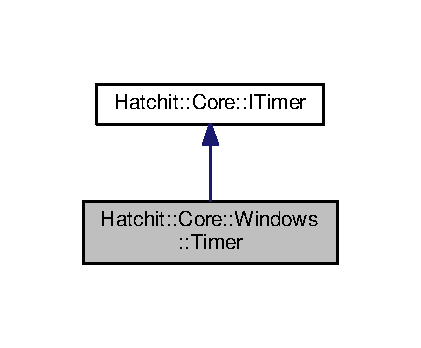
\includegraphics[width=202pt]{classHatchit_1_1Core_1_1Windows_1_1Timer__inherit__graph}
\end{center}
\end{figure}


Collaboration diagram for Hatchit\+:\+:Core\+:\+:Windows\+:\+:Timer\+:
\nopagebreak
\begin{figure}[H]
\begin{center}
\leavevmode
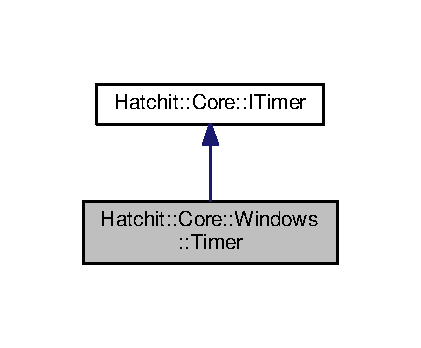
\includegraphics[width=202pt]{classHatchit_1_1Core_1_1Windows_1_1Timer__coll__graph}
\end{center}
\end{figure}
\subsection*{Public Member Functions}
\begin{DoxyCompactItemize}
\item 
virtual void \hyperlink{classHatchit_1_1Core_1_1Windows_1_1Timer_a6441edbd90a09f4cfbca01fafd4d0aff}{Start} () override
\begin{DoxyCompactList}\small\item\em Starts tracking time from moment this function is called. \end{DoxyCompactList}\item 
virtual void \hyperlink{classHatchit_1_1Core_1_1Windows_1_1Timer_ae1879dac284fc160b0322f5a57aa8ae3}{Tick} () override
\begin{DoxyCompactList}\small\item\em Calculates the delta time and total time. \end{DoxyCompactList}\item 
virtual void \hyperlink{classHatchit_1_1Core_1_1Windows_1_1Timer_a1d9f06759a7a48e807d4b2a0254e7dbc}{Stop} () override
\begin{DoxyCompactList}\small\item\em Stops timer. \end{DoxyCompactList}\item 
virtual void \hyperlink{classHatchit_1_1Core_1_1Windows_1_1Timer_a464c6b3e3017867bd387a8fb477ad186}{Reset} () override
\begin{DoxyCompactList}\small\item\em Resets the timer data. \end{DoxyCompactList}\item 
virtual float \hyperlink{classHatchit_1_1Core_1_1Windows_1_1Timer_a4cda627adbe26e6f2b5438681063995e}{Elapsed\+Time} () const override
\begin{DoxyCompactList}\small\item\em Gets elapsed time (in seconds) \end{DoxyCompactList}\item 
virtual float \hyperlink{classHatchit_1_1Core_1_1Windows_1_1Timer_a5cc4dcb2292ef3e12a5855990c296ab7}{Total\+Time} () const override
\begin{DoxyCompactList}\small\item\em Gets total time (in seconds) \end{DoxyCompactList}\item 
virtual float \hyperlink{classHatchit_1_1Core_1_1Windows_1_1Timer_a79a80293593eb0d0785e896bbf7c934b}{Delta\+Time} () const override
\begin{DoxyCompactList}\small\item\em Gets delta time (in seconds) \end{DoxyCompactList}\end{DoxyCompactItemize}
\subsection*{Additional Inherited Members}


\subsection{Detailed Description}
Defines class to track elapsed time. 

Defines class to track elapsed time. \hyperlink{classHatchit_1_1Core_1_1Windows_1_1Timer}{Timer} is specific to \hyperlink{namespaceWindows}{Windows} 

Definition at line 46 of file ht\+\_\+windowstimer.\+h.



\subsection{Member Function Documentation}
\index{Hatchit\+::\+Core\+::\+Windows\+::\+Timer@{Hatchit\+::\+Core\+::\+Windows\+::\+Timer}!Delta\+Time@{Delta\+Time}}
\index{Delta\+Time@{Delta\+Time}!Hatchit\+::\+Core\+::\+Windows\+::\+Timer@{Hatchit\+::\+Core\+::\+Windows\+::\+Timer}}
\subsubsection[{\texorpdfstring{Delta\+Time() const override}{DeltaTime() const override}}]{\setlength{\rightskip}{0pt plus 5cm}virtual float Hatchit\+::\+Core\+::\+Windows\+::\+Timer\+::\+Delta\+Time (
\begin{DoxyParamCaption}
{}
\end{DoxyParamCaption}
) const\hspace{0.3cm}{\ttfamily [override]}, {\ttfamily [virtual]}}\hypertarget{classHatchit_1_1Core_1_1Windows_1_1Timer_a79a80293593eb0d0785e896bbf7c934b}{}\label{classHatchit_1_1Core_1_1Windows_1_1Timer_a79a80293593eb0d0785e896bbf7c934b}


Gets delta time (in seconds) 

Returns delta time (in seconds) between last two ticks of timer. 

Implements \hyperlink{classHatchit_1_1Core_1_1ITimer_a201d0dd1503b393ea7c1e1acfb402cd5}{Hatchit\+::\+Core\+::\+I\+Timer}.

\index{Hatchit\+::\+Core\+::\+Windows\+::\+Timer@{Hatchit\+::\+Core\+::\+Windows\+::\+Timer}!Elapsed\+Time@{Elapsed\+Time}}
\index{Elapsed\+Time@{Elapsed\+Time}!Hatchit\+::\+Core\+::\+Windows\+::\+Timer@{Hatchit\+::\+Core\+::\+Windows\+::\+Timer}}
\subsubsection[{\texorpdfstring{Elapsed\+Time() const override}{ElapsedTime() const override}}]{\setlength{\rightskip}{0pt plus 5cm}virtual float Hatchit\+::\+Core\+::\+Windows\+::\+Timer\+::\+Elapsed\+Time (
\begin{DoxyParamCaption}
{}
\end{DoxyParamCaption}
) const\hspace{0.3cm}{\ttfamily [override]}, {\ttfamily [virtual]}}\hypertarget{classHatchit_1_1Core_1_1Windows_1_1Timer_a4cda627adbe26e6f2b5438681063995e}{}\label{classHatchit_1_1Core_1_1Windows_1_1Timer_a4cda627adbe26e6f2b5438681063995e}


Gets elapsed time (in seconds) 

Returns elapsed time (in seconds) between \hyperlink{classHatchit_1_1Core_1_1Windows_1_1Timer_a6441edbd90a09f4cfbca01fafd4d0aff}{Start()} and \hyperlink{classHatchit_1_1Core_1_1Windows_1_1Timer_a1d9f06759a7a48e807d4b2a0254e7dbc}{Stop()} calls. 

Implements \hyperlink{classHatchit_1_1Core_1_1ITimer_aef2f629b7e527640a62af97dad17dcb2}{Hatchit\+::\+Core\+::\+I\+Timer}.

\index{Hatchit\+::\+Core\+::\+Windows\+::\+Timer@{Hatchit\+::\+Core\+::\+Windows\+::\+Timer}!Reset@{Reset}}
\index{Reset@{Reset}!Hatchit\+::\+Core\+::\+Windows\+::\+Timer@{Hatchit\+::\+Core\+::\+Windows\+::\+Timer}}
\subsubsection[{\texorpdfstring{Reset() override}{Reset() override}}]{\setlength{\rightskip}{0pt plus 5cm}virtual void Hatchit\+::\+Core\+::\+Windows\+::\+Timer\+::\+Reset (
\begin{DoxyParamCaption}
{}
\end{DoxyParamCaption}
)\hspace{0.3cm}{\ttfamily [override]}, {\ttfamily [virtual]}}\hypertarget{classHatchit_1_1Core_1_1Windows_1_1Timer_a464c6b3e3017867bd387a8fb477ad186}{}\label{classHatchit_1_1Core_1_1Windows_1_1Timer_a464c6b3e3017867bd387a8fb477ad186}


Resets the timer data. 

If timer is currently running, delta time will be calculated between the tick this function is called and the tick that \hyperlink{classHatchit_1_1Core_1_1Windows_1_1Timer_ae1879dac284fc160b0322f5a57aa8ae3}{Tick()} is called. 

Implements \hyperlink{classHatchit_1_1Core_1_1ITimer_a4f6fc1ec97ef9345d64e75bdeadcdad2}{Hatchit\+::\+Core\+::\+I\+Timer}.

\index{Hatchit\+::\+Core\+::\+Windows\+::\+Timer@{Hatchit\+::\+Core\+::\+Windows\+::\+Timer}!Start@{Start}}
\index{Start@{Start}!Hatchit\+::\+Core\+::\+Windows\+::\+Timer@{Hatchit\+::\+Core\+::\+Windows\+::\+Timer}}
\subsubsection[{\texorpdfstring{Start() override}{Start() override}}]{\setlength{\rightskip}{0pt plus 5cm}virtual void Hatchit\+::\+Core\+::\+Windows\+::\+Timer\+::\+Start (
\begin{DoxyParamCaption}
{}
\end{DoxyParamCaption}
)\hspace{0.3cm}{\ttfamily [override]}, {\ttfamily [virtual]}}\hypertarget{classHatchit_1_1Core_1_1Windows_1_1Timer_a6441edbd90a09f4cfbca01fafd4d0aff}{}\label{classHatchit_1_1Core_1_1Windows_1_1Timer_a6441edbd90a09f4cfbca01fafd4d0aff}


Starts tracking time from moment this function is called. 

Starts tracking time from moment this function is called. 

Implements \hyperlink{classHatchit_1_1Core_1_1ITimer_abf16ebbb5a924fc20cf3099280f74cf7}{Hatchit\+::\+Core\+::\+I\+Timer}.

\index{Hatchit\+::\+Core\+::\+Windows\+::\+Timer@{Hatchit\+::\+Core\+::\+Windows\+::\+Timer}!Stop@{Stop}}
\index{Stop@{Stop}!Hatchit\+::\+Core\+::\+Windows\+::\+Timer@{Hatchit\+::\+Core\+::\+Windows\+::\+Timer}}
\subsubsection[{\texorpdfstring{Stop() override}{Stop() override}}]{\setlength{\rightskip}{0pt plus 5cm}virtual void Hatchit\+::\+Core\+::\+Windows\+::\+Timer\+::\+Stop (
\begin{DoxyParamCaption}
{}
\end{DoxyParamCaption}
)\hspace{0.3cm}{\ttfamily [override]}, {\ttfamily [virtual]}}\hypertarget{classHatchit_1_1Core_1_1Windows_1_1Timer_a1d9f06759a7a48e807d4b2a0254e7dbc}{}\label{classHatchit_1_1Core_1_1Windows_1_1Timer_a1d9f06759a7a48e807d4b2a0254e7dbc}


Stops timer. 

Stops tracking timing information 

Implements \hyperlink{classHatchit_1_1Core_1_1ITimer_a3bb9bec5874fd1c706ced3ba8033c761}{Hatchit\+::\+Core\+::\+I\+Timer}.

\index{Hatchit\+::\+Core\+::\+Windows\+::\+Timer@{Hatchit\+::\+Core\+::\+Windows\+::\+Timer}!Tick@{Tick}}
\index{Tick@{Tick}!Hatchit\+::\+Core\+::\+Windows\+::\+Timer@{Hatchit\+::\+Core\+::\+Windows\+::\+Timer}}
\subsubsection[{\texorpdfstring{Tick() override}{Tick() override}}]{\setlength{\rightskip}{0pt plus 5cm}virtual void Hatchit\+::\+Core\+::\+Windows\+::\+Timer\+::\+Tick (
\begin{DoxyParamCaption}
{}
\end{DoxyParamCaption}
)\hspace{0.3cm}{\ttfamily [override]}, {\ttfamily [virtual]}}\hypertarget{classHatchit_1_1Core_1_1Windows_1_1Timer_ae1879dac284fc160b0322f5a57aa8ae3}{}\label{classHatchit_1_1Core_1_1Windows_1_1Timer_ae1879dac284fc160b0322f5a57aa8ae3}


Calculates the delta time and total time. 

Calculates the delta time between this tick and the last tick, or the last reset, depending on which happened more recently. Also recalculates the total time by accruing the calculated delta time into the total time. 

Implements \hyperlink{classHatchit_1_1Core_1_1ITimer_a6969cb6203be6fd3d3a002146bb55fa1}{Hatchit\+::\+Core\+::\+I\+Timer}.

\index{Hatchit\+::\+Core\+::\+Windows\+::\+Timer@{Hatchit\+::\+Core\+::\+Windows\+::\+Timer}!Total\+Time@{Total\+Time}}
\index{Total\+Time@{Total\+Time}!Hatchit\+::\+Core\+::\+Windows\+::\+Timer@{Hatchit\+::\+Core\+::\+Windows\+::\+Timer}}
\subsubsection[{\texorpdfstring{Total\+Time() const override}{TotalTime() const override}}]{\setlength{\rightskip}{0pt plus 5cm}virtual float Hatchit\+::\+Core\+::\+Windows\+::\+Timer\+::\+Total\+Time (
\begin{DoxyParamCaption}
{}
\end{DoxyParamCaption}
) const\hspace{0.3cm}{\ttfamily [override]}, {\ttfamily [virtual]}}\hypertarget{classHatchit_1_1Core_1_1Windows_1_1Timer_a5cc4dcb2292ef3e12a5855990c296ab7}{}\label{classHatchit_1_1Core_1_1Windows_1_1Timer_a5cc4dcb2292ef3e12a5855990c296ab7}


Gets total time (in seconds) 

Returns total time between when timer was started and last tick. 

Implements \hyperlink{classHatchit_1_1Core_1_1ITimer_af5d9551ef9a0a98591f823b014efca11}{Hatchit\+::\+Core\+::\+I\+Timer}.



The documentation for this class was generated from the following file\+:\begin{DoxyCompactItemize}
\item 
/home/debunez/\+Git\+Hub/\+Hatchit\+Editor/\+Hatchit/\+Hatchit\+Core/include/windows/\hyperlink{ht__windowstimer_8h}{ht\+\_\+windowstimer.\+h}\end{DoxyCompactItemize}

\hypertarget{classHatchit_1_1Core_1_1Linux_1_1Timer}{}\section{Hatchit\+:\+:Core\+:\+:Linux\+:\+:Timer Class Reference}
\label{classHatchit_1_1Core_1_1Linux_1_1Timer}\index{Hatchit\+::\+Core\+::\+Linux\+::\+Timer@{Hatchit\+::\+Core\+::\+Linux\+::\+Timer}}


Defines class to track elapsed time.  




{\ttfamily \#include $<$ht\+\_\+linuxtimer.\+h$>$}



Inheritance diagram for Hatchit\+:\+:Core\+:\+:Linux\+:\+:Timer\+:
\nopagebreak
\begin{figure}[H]
\begin{center}
\leavevmode
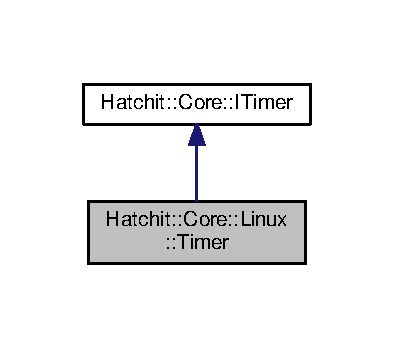
\includegraphics[width=189pt]{classHatchit_1_1Core_1_1Linux_1_1Timer__inherit__graph}
\end{center}
\end{figure}


Collaboration diagram for Hatchit\+:\+:Core\+:\+:Linux\+:\+:Timer\+:
\nopagebreak
\begin{figure}[H]
\begin{center}
\leavevmode
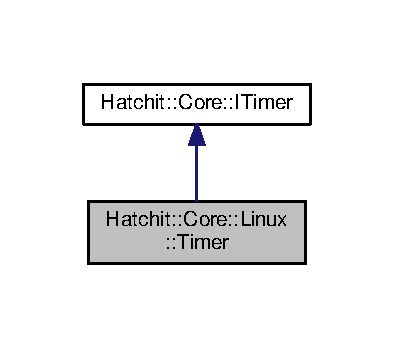
\includegraphics[width=189pt]{classHatchit_1_1Core_1_1Linux_1_1Timer__coll__graph}
\end{center}
\end{figure}
\subsection*{Public Member Functions}
\begin{DoxyCompactItemize}
\item 
virtual void \hyperlink{classHatchit_1_1Core_1_1Linux_1_1Timer_ad71a11915c848a40be11b2a2a1c24375}{Start} () override
\begin{DoxyCompactList}\small\item\em Starts tracking time from moment this function is called. \end{DoxyCompactList}\item 
virtual void \hyperlink{classHatchit_1_1Core_1_1Linux_1_1Timer_aafd5b502c0fda46aad2f38b47a6974d6}{Tick} () override
\begin{DoxyCompactList}\small\item\em Calculates the delta time and total time. \end{DoxyCompactList}\item 
virtual void \hyperlink{classHatchit_1_1Core_1_1Linux_1_1Timer_a93adf56776127d8c3215024f6566837b}{Stop} () override
\begin{DoxyCompactList}\small\item\em Stops timer. \end{DoxyCompactList}\item 
virtual void \hyperlink{classHatchit_1_1Core_1_1Linux_1_1Timer_a1159f074a5290718acee991decd80af3}{Reset} () override
\begin{DoxyCompactList}\small\item\em Resets the timer data. \end{DoxyCompactList}\item 
virtual float \hyperlink{classHatchit_1_1Core_1_1Linux_1_1Timer_aa8e7a94df99e3953eebbb0d08d1dd8a2}{Elapsed\+Time} () const override
\begin{DoxyCompactList}\small\item\em Gets elapsed time (in seconds) \end{DoxyCompactList}\item 
virtual float \hyperlink{classHatchit_1_1Core_1_1Linux_1_1Timer_a9ca1371d09e3fd4ddb72ea4f6b9fb9d9}{Total\+Time} () const override
\begin{DoxyCompactList}\small\item\em Gets total time (in seconds) \end{DoxyCompactList}\item 
virtual float \hyperlink{classHatchit_1_1Core_1_1Linux_1_1Timer_aefd9ad0a2297d03e3877c0c6c900bd1c}{Delta\+Time} () const override
\begin{DoxyCompactList}\small\item\em Gets delta time (in seconds) \end{DoxyCompactList}\end{DoxyCompactItemize}
\subsection*{Additional Inherited Members}


\subsection{Detailed Description}
Defines class to track elapsed time. 

Defines class to track elapsed time. \hyperlink{classHatchit_1_1Core_1_1Linux_1_1Timer}{Timer} is specific to \hyperlink{namespaceLinux}{Linux} 

Definition at line 48 of file ht\+\_\+linuxtimer.\+h.



\subsection{Member Function Documentation}
\index{Hatchit\+::\+Core\+::\+Linux\+::\+Timer@{Hatchit\+::\+Core\+::\+Linux\+::\+Timer}!Delta\+Time@{Delta\+Time}}
\index{Delta\+Time@{Delta\+Time}!Hatchit\+::\+Core\+::\+Linux\+::\+Timer@{Hatchit\+::\+Core\+::\+Linux\+::\+Timer}}
\subsubsection[{\texorpdfstring{Delta\+Time() const override}{DeltaTime() const override}}]{\setlength{\rightskip}{0pt plus 5cm}virtual float Hatchit\+::\+Core\+::\+Linux\+::\+Timer\+::\+Delta\+Time (
\begin{DoxyParamCaption}
{}
\end{DoxyParamCaption}
) const\hspace{0.3cm}{\ttfamily [override]}, {\ttfamily [virtual]}}\hypertarget{classHatchit_1_1Core_1_1Linux_1_1Timer_aefd9ad0a2297d03e3877c0c6c900bd1c}{}\label{classHatchit_1_1Core_1_1Linux_1_1Timer_aefd9ad0a2297d03e3877c0c6c900bd1c}


Gets delta time (in seconds) 

Returns delta time (in seconds) between last two ticks of timer. 

Implements \hyperlink{classHatchit_1_1Core_1_1ITimer_a201d0dd1503b393ea7c1e1acfb402cd5}{Hatchit\+::\+Core\+::\+I\+Timer}.

\index{Hatchit\+::\+Core\+::\+Linux\+::\+Timer@{Hatchit\+::\+Core\+::\+Linux\+::\+Timer}!Elapsed\+Time@{Elapsed\+Time}}
\index{Elapsed\+Time@{Elapsed\+Time}!Hatchit\+::\+Core\+::\+Linux\+::\+Timer@{Hatchit\+::\+Core\+::\+Linux\+::\+Timer}}
\subsubsection[{\texorpdfstring{Elapsed\+Time() const override}{ElapsedTime() const override}}]{\setlength{\rightskip}{0pt plus 5cm}virtual float Hatchit\+::\+Core\+::\+Linux\+::\+Timer\+::\+Elapsed\+Time (
\begin{DoxyParamCaption}
{}
\end{DoxyParamCaption}
) const\hspace{0.3cm}{\ttfamily [override]}, {\ttfamily [virtual]}}\hypertarget{classHatchit_1_1Core_1_1Linux_1_1Timer_aa8e7a94df99e3953eebbb0d08d1dd8a2}{}\label{classHatchit_1_1Core_1_1Linux_1_1Timer_aa8e7a94df99e3953eebbb0d08d1dd8a2}


Gets elapsed time (in seconds) 

Returns elapsed time (in seconds) between \hyperlink{classHatchit_1_1Core_1_1Linux_1_1Timer_ad71a11915c848a40be11b2a2a1c24375}{Start()} and \hyperlink{classHatchit_1_1Core_1_1Linux_1_1Timer_a93adf56776127d8c3215024f6566837b}{Stop()} calls. 

Implements \hyperlink{classHatchit_1_1Core_1_1ITimer_aef2f629b7e527640a62af97dad17dcb2}{Hatchit\+::\+Core\+::\+I\+Timer}.

\index{Hatchit\+::\+Core\+::\+Linux\+::\+Timer@{Hatchit\+::\+Core\+::\+Linux\+::\+Timer}!Reset@{Reset}}
\index{Reset@{Reset}!Hatchit\+::\+Core\+::\+Linux\+::\+Timer@{Hatchit\+::\+Core\+::\+Linux\+::\+Timer}}
\subsubsection[{\texorpdfstring{Reset() override}{Reset() override}}]{\setlength{\rightskip}{0pt plus 5cm}virtual void Hatchit\+::\+Core\+::\+Linux\+::\+Timer\+::\+Reset (
\begin{DoxyParamCaption}
{}
\end{DoxyParamCaption}
)\hspace{0.3cm}{\ttfamily [override]}, {\ttfamily [virtual]}}\hypertarget{classHatchit_1_1Core_1_1Linux_1_1Timer_a1159f074a5290718acee991decd80af3}{}\label{classHatchit_1_1Core_1_1Linux_1_1Timer_a1159f074a5290718acee991decd80af3}


Resets the timer data. 

If timer is currently running, delta time will be calculated between the tick this function is called and the tick that \hyperlink{classHatchit_1_1Core_1_1Linux_1_1Timer_aafd5b502c0fda46aad2f38b47a6974d6}{Tick()} is called. 

Implements \hyperlink{classHatchit_1_1Core_1_1ITimer_a4f6fc1ec97ef9345d64e75bdeadcdad2}{Hatchit\+::\+Core\+::\+I\+Timer}.

\index{Hatchit\+::\+Core\+::\+Linux\+::\+Timer@{Hatchit\+::\+Core\+::\+Linux\+::\+Timer}!Start@{Start}}
\index{Start@{Start}!Hatchit\+::\+Core\+::\+Linux\+::\+Timer@{Hatchit\+::\+Core\+::\+Linux\+::\+Timer}}
\subsubsection[{\texorpdfstring{Start() override}{Start() override}}]{\setlength{\rightskip}{0pt plus 5cm}virtual void Hatchit\+::\+Core\+::\+Linux\+::\+Timer\+::\+Start (
\begin{DoxyParamCaption}
{}
\end{DoxyParamCaption}
)\hspace{0.3cm}{\ttfamily [override]}, {\ttfamily [virtual]}}\hypertarget{classHatchit_1_1Core_1_1Linux_1_1Timer_ad71a11915c848a40be11b2a2a1c24375}{}\label{classHatchit_1_1Core_1_1Linux_1_1Timer_ad71a11915c848a40be11b2a2a1c24375}


Starts tracking time from moment this function is called. 

Starts tracking time from moment this function is called. 

Implements \hyperlink{classHatchit_1_1Core_1_1ITimer_abf16ebbb5a924fc20cf3099280f74cf7}{Hatchit\+::\+Core\+::\+I\+Timer}.

\index{Hatchit\+::\+Core\+::\+Linux\+::\+Timer@{Hatchit\+::\+Core\+::\+Linux\+::\+Timer}!Stop@{Stop}}
\index{Stop@{Stop}!Hatchit\+::\+Core\+::\+Linux\+::\+Timer@{Hatchit\+::\+Core\+::\+Linux\+::\+Timer}}
\subsubsection[{\texorpdfstring{Stop() override}{Stop() override}}]{\setlength{\rightskip}{0pt plus 5cm}virtual void Hatchit\+::\+Core\+::\+Linux\+::\+Timer\+::\+Stop (
\begin{DoxyParamCaption}
{}
\end{DoxyParamCaption}
)\hspace{0.3cm}{\ttfamily [override]}, {\ttfamily [virtual]}}\hypertarget{classHatchit_1_1Core_1_1Linux_1_1Timer_a93adf56776127d8c3215024f6566837b}{}\label{classHatchit_1_1Core_1_1Linux_1_1Timer_a93adf56776127d8c3215024f6566837b}


Stops timer. 

Stops tracking timing information 

Implements \hyperlink{classHatchit_1_1Core_1_1ITimer_a3bb9bec5874fd1c706ced3ba8033c761}{Hatchit\+::\+Core\+::\+I\+Timer}.

\index{Hatchit\+::\+Core\+::\+Linux\+::\+Timer@{Hatchit\+::\+Core\+::\+Linux\+::\+Timer}!Tick@{Tick}}
\index{Tick@{Tick}!Hatchit\+::\+Core\+::\+Linux\+::\+Timer@{Hatchit\+::\+Core\+::\+Linux\+::\+Timer}}
\subsubsection[{\texorpdfstring{Tick() override}{Tick() override}}]{\setlength{\rightskip}{0pt plus 5cm}virtual void Hatchit\+::\+Core\+::\+Linux\+::\+Timer\+::\+Tick (
\begin{DoxyParamCaption}
{}
\end{DoxyParamCaption}
)\hspace{0.3cm}{\ttfamily [override]}, {\ttfamily [virtual]}}\hypertarget{classHatchit_1_1Core_1_1Linux_1_1Timer_aafd5b502c0fda46aad2f38b47a6974d6}{}\label{classHatchit_1_1Core_1_1Linux_1_1Timer_aafd5b502c0fda46aad2f38b47a6974d6}


Calculates the delta time and total time. 

Calculates the delta time between this tick and the last tick, or the last reset, depending on which happened more recently. Also recalculates the total time by accruing the calculated delta time into the total time. 

Implements \hyperlink{classHatchit_1_1Core_1_1ITimer_a6969cb6203be6fd3d3a002146bb55fa1}{Hatchit\+::\+Core\+::\+I\+Timer}.

\index{Hatchit\+::\+Core\+::\+Linux\+::\+Timer@{Hatchit\+::\+Core\+::\+Linux\+::\+Timer}!Total\+Time@{Total\+Time}}
\index{Total\+Time@{Total\+Time}!Hatchit\+::\+Core\+::\+Linux\+::\+Timer@{Hatchit\+::\+Core\+::\+Linux\+::\+Timer}}
\subsubsection[{\texorpdfstring{Total\+Time() const override}{TotalTime() const override}}]{\setlength{\rightskip}{0pt plus 5cm}virtual float Hatchit\+::\+Core\+::\+Linux\+::\+Timer\+::\+Total\+Time (
\begin{DoxyParamCaption}
{}
\end{DoxyParamCaption}
) const\hspace{0.3cm}{\ttfamily [override]}, {\ttfamily [virtual]}}\hypertarget{classHatchit_1_1Core_1_1Linux_1_1Timer_a9ca1371d09e3fd4ddb72ea4f6b9fb9d9}{}\label{classHatchit_1_1Core_1_1Linux_1_1Timer_a9ca1371d09e3fd4ddb72ea4f6b9fb9d9}


Gets total time (in seconds) 

Returns total time between when timer was started and last tick. 

Implements \hyperlink{classHatchit_1_1Core_1_1ITimer_af5d9551ef9a0a98591f823b014efca11}{Hatchit\+::\+Core\+::\+I\+Timer}.



The documentation for this class was generated from the following file\+:\begin{DoxyCompactItemize}
\item 
/home/debunez/\+Git\+Hub/\+Hatchit\+Editor/\+Hatchit/\+Hatchit\+Core/include/linux/\hyperlink{ht__linuxtimer_8h}{ht\+\_\+linuxtimer.\+h}\end{DoxyCompactItemize}

\chapter{File Documentation}
\hypertarget{ht__bitfield_8h}{}\section{/home/debunez/\+Git\+Hub/\+Hatchit\+Editor/\+Hatchit/\+Hatchit\+Core/include/ht\+\_\+bitfield.h File Reference}
\label{ht__bitfield_8h}\index{/home/debunez/\+Git\+Hub/\+Hatchit\+Editor/\+Hatchit/\+Hatchit\+Core/include/ht\+\_\+bitfield.\+h@{/home/debunez/\+Git\+Hub/\+Hatchit\+Editor/\+Hatchit/\+Hatchit\+Core/include/ht\+\_\+bitfield.\+h}}


Bit\+Field class definition.  


{\ttfamily \#include $<$type\+\_\+traits$>$}\\*
{\ttfamily \#include $<$ht\+\_\+bitfield.\+inl$>$}\\*
Include dependency graph for ht\+\_\+bitfield.\+h\+:
\nopagebreak
\begin{figure}[H]
\begin{center}
\leavevmode
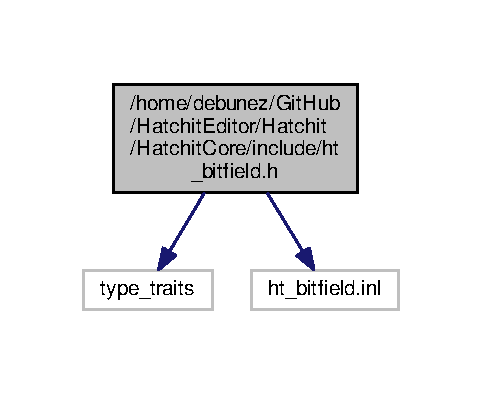
\includegraphics[width=232pt]{ht__bitfield_8h__incl}
\end{center}
\end{figure}
\subsection*{Classes}
\begin{DoxyCompactItemize}
\item 
class \hyperlink{classHatchit_1_1Core_1_1BitFlag}{Hatchit\+::\+Core\+::\+Bit\+Flag}
\begin{DoxyCompactList}\small\item\em A class that represents a single bit flag. \end{DoxyCompactList}\item 
class \hyperlink{classHatchit_1_1Core_1_1BitField}{Hatchit\+::\+Core\+::\+Bit\+Field$<$ Enum $>$}
\begin{DoxyCompactList}\small\item\em A class that represents an array of bitflags for a given enum. \end{DoxyCompactList}\end{DoxyCompactItemize}
\subsection*{Namespaces}
\begin{DoxyCompactItemize}
\item 
 \hyperlink{namespaceHatchit}{Hatchit}
\begin{DoxyCompactList}\small\item\em Engine global layer. \end{DoxyCompactList}\item 
 \hyperlink{namespaceHatchit_1_1Core}{Hatchit\+::\+Core}
\begin{DoxyCompactList}\small\item\em Engine utility layer. \end{DoxyCompactList}\end{DoxyCompactItemize}


\subsection{Detailed Description}
Bit\+Field class definition. 

\hyperlink{namespaceHatchit}{Hatchit} Engine Copyright(c) 2015-\/2016 Third-\/\+Degree

G\+NU Lesser General Public License This file may be used under the terms of the G\+NU Lesser General Public License version 3 as published by the Free Software Foundation and appearing in the file L\+I\+C\+E\+N\+S\+E.\+L\+G\+P\+Lv3 included in the packaging of this file. Please review the following information to ensure the G\+NU Lesser General Public License requirements will be met\+: \href{https://www.gnu.org/licenses/lgpl.html}{\tt https\+://www.\+gnu.\+org/licenses/lgpl.\+html}

\begin{DoxyAuthor}{Author}
Third-\/\+Degree contributors (\href{https://github.com/thirddegree}{\tt https\+://github.\+com/thirddegree})
\end{DoxyAuthor}
This file contains definition for Bit\+Field class 
\hypertarget{ht__debug_8h}{}\section{/home/debunez/\+Git\+Hub/\+Hatchit\+Editor/\+Hatchit/\+Hatchit\+Core/include/ht\+\_\+debug.h File Reference}
\label{ht__debug_8h}\index{/home/debunez/\+Git\+Hub/\+Hatchit\+Editor/\+Hatchit/\+Hatchit\+Core/include/ht\+\_\+debug.\+h@{/home/debunez/\+Git\+Hub/\+Hatchit\+Editor/\+Hatchit/\+Hatchit\+Core/include/ht\+\_\+debug.\+h}}


Defines various debug utilities.  


{\ttfamily \#include $<$string$>$}\\*
{\ttfamily \#include $<$fstream$>$}\\*
{\ttfamily \#include $<$memory$>$}\\*
{\ttfamily \#include $<$functional$>$}\\*
{\ttfamily \#include $<$ht\+\_\+platform.\+h$>$}\\*
{\ttfamily \#include $<$format.\+h$>$}\\*
{\ttfamily \#include $<$ht\+\_\+debug.\+inl$>$}\\*
Include dependency graph for ht\+\_\+debug.\+h\+:
\nopagebreak
\begin{figure}[H]
\begin{center}
\leavevmode
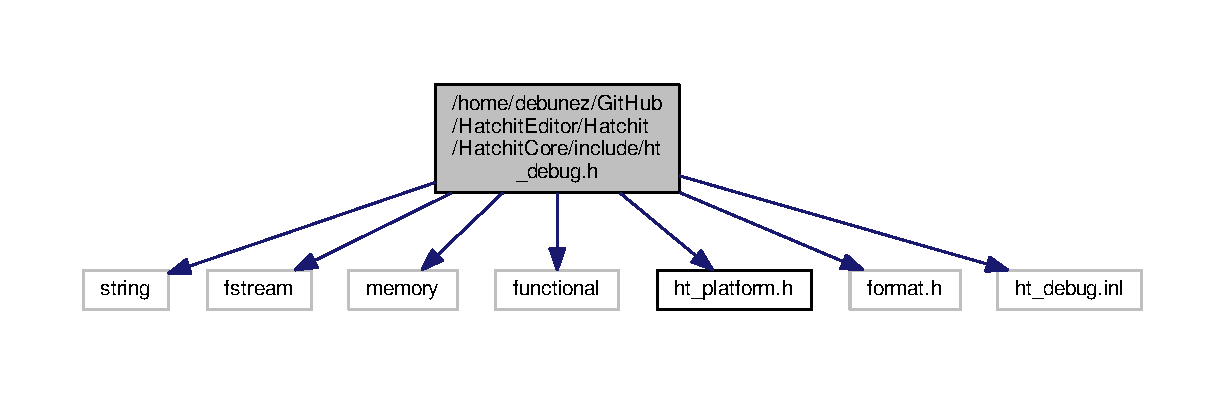
\includegraphics[width=350pt]{ht__debug_8h__incl}
\end{center}
\end{figure}
\subsection*{Classes}
\begin{DoxyCompactItemize}
\item 
class \hyperlink{classHatchit_1_1Core_1_1Debug}{Hatchit\+::\+Core\+::\+Debug}
\begin{DoxyCompactList}\small\item\em Defines a static debug class. \end{DoxyCompactList}\end{DoxyCompactItemize}
\subsection*{Namespaces}
\begin{DoxyCompactItemize}
\item 
 \hyperlink{namespaceHatchit}{Hatchit}
\begin{DoxyCompactList}\small\item\em Engine global layer. \end{DoxyCompactList}\item 
 \hyperlink{namespaceHatchit_1_1Core}{Hatchit\+::\+Core}
\begin{DoxyCompactList}\small\item\em Engine utility layer. \end{DoxyCompactList}\end{DoxyCompactItemize}
\subsection*{Macros}
\begin{DoxyCompactItemize}
\item 
\#define \hyperlink{ht__debug_8h_ab7a5b69f1ca1fef28b1f902c9b87f69a}{H\+T\+\_\+\+S\+T\+R\+I\+N\+G\+I\+FY}(x)~\#x
\item 
\#define \hyperlink{ht__debug_8h_a81c357f9aa0e9986119e70c2efe94f97}{H\+T\+\_\+\+S\+F\+Y\+\_\+}(x)~\hyperlink{ht__debug_8h_ab7a5b69f1ca1fef28b1f902c9b87f69a}{H\+T\+\_\+\+S\+T\+R\+I\+N\+G\+I\+FY}(x)
\item 
\#define \hyperlink{ht__debug_8h_a35aeff282ae4e9c793cf62a14d8f9f2b}{H\+T\+\_\+\+F\+U\+N\+C\+T\+I\+ON}~\+\_\+\+\_\+\+F\+U\+N\+C\+S\+I\+G\+\_\+\+\_\+
\item 
\#define \hyperlink{ht__debug_8h_a20152bf56a631aa09fea1c8de710a369}{H\+T\+\_\+\+D\+E\+B\+U\+G\+\_\+\+P\+R\+I\+N\+TF}(message, ...)
\item 
\#define {\bfseries H\+T\+\_\+\+I\+N\+F\+O\+\_\+\+P\+R\+I\+N\+TF}(message, ...)~\hyperlink{classHatchit_1_1Core_1_1Debug_a7a97b3ab2f6608e2c2985905cb20fe3b}{Hatchit\+::\+Core\+::\+Debug\+::\+Log}(Hatchit\+::\+Core\+::\+Debug\+::\+Log\+Severity\+::\+Info, message, \#\#\+\_\+\+\_\+\+V\+A\+\_\+\+A\+R\+G\+S\+\_\+\+\_\+)\hypertarget{ht__debug_8h_ac552600486f322d2bc1c95789ab6b966}{}\label{ht__debug_8h_ac552600486f322d2bc1c95789ab6b966}

\item 
\#define {\bfseries H\+T\+\_\+\+W\+A\+R\+N\+I\+N\+G\+\_\+\+P\+R\+I\+N\+TF}(message, ...)~\hyperlink{classHatchit_1_1Core_1_1Debug_a7a97b3ab2f6608e2c2985905cb20fe3b}{Hatchit\+::\+Core\+::\+Debug\+::\+Log}(Hatchit\+::\+Core\+::\+Debug\+::\+Log\+Severity\+::\+Warning, message, \#\#\+\_\+\+\_\+\+V\+A\+\_\+\+A\+R\+G\+S\+\_\+\+\_\+)\hypertarget{ht__debug_8h_ab9688d27398d70bf565873394e05f1aa}{}\label{ht__debug_8h_ab9688d27398d70bf565873394e05f1aa}

\item 
\#define {\bfseries H\+T\+\_\+\+E\+R\+R\+O\+R\+\_\+\+P\+R\+I\+N\+TF}(message, ...)~\hyperlink{classHatchit_1_1Core_1_1Debug_a7a97b3ab2f6608e2c2985905cb20fe3b}{Hatchit\+::\+Core\+::\+Debug\+::\+Log}(Hatchit\+::\+Core\+::\+Debug\+::\+Log\+Severity\+::\+Error, message, \#\#\+\_\+\+\_\+\+V\+A\+\_\+\+A\+R\+G\+S\+\_\+\+\_\+)\hypertarget{ht__debug_8h_a2eb37db6d9c45b2678760d12791e2709}{}\label{ht__debug_8h_a2eb37db6d9c45b2678760d12791e2709}

\end{DoxyCompactItemize}


\subsection{Detailed Description}
Defines various debug utilities. 

\hyperlink{namespaceHatchit}{Hatchit} Engine Copyright(c) 2015-\/2016 Third-\/\+Degree

G\+NU Lesser General Public License This file may be used under the terms of the G\+NU Lesser General Public License version 3 as published by the Free Software Foundation and appearing in the file L\+I\+C\+E\+N\+S\+E.\+L\+G\+P\+Lv3 included in the packaging of this file. Please review the following information to ensure the G\+NU Lesser General Public License requirements will be met\+: \href{https://www.gnu.org/licenses/lgpl.html}{\tt https\+://www.\+gnu.\+org/licenses/lgpl.\+html}

\begin{DoxyAuthor}{Author}
Matt Guerrette (\href{mailto:direct3Dtutorials@gmail.com}{\tt direct3\+Dtutorials@gmail.\+com}) 

Third-\/\+Degree contributors (\href{https://github.com/thirddegree}{\tt https\+://github.\+com/thirddegree})
\end{DoxyAuthor}
This file contains various debug utility functions and macros 

\subsection{Macro Definition Documentation}
\index{ht\+\_\+debug.\+h@{ht\+\_\+debug.\+h}!H\+T\+\_\+\+D\+E\+B\+U\+G\+\_\+\+P\+R\+I\+N\+TF@{H\+T\+\_\+\+D\+E\+B\+U\+G\+\_\+\+P\+R\+I\+N\+TF}}
\index{H\+T\+\_\+\+D\+E\+B\+U\+G\+\_\+\+P\+R\+I\+N\+TF@{H\+T\+\_\+\+D\+E\+B\+U\+G\+\_\+\+P\+R\+I\+N\+TF}!ht\+\_\+debug.\+h@{ht\+\_\+debug.\+h}}
\subsubsection[{\texorpdfstring{H\+T\+\_\+\+D\+E\+B\+U\+G\+\_\+\+P\+R\+I\+N\+TF}{HT_DEBUG_PRINTF}}]{\setlength{\rightskip}{0pt plus 5cm}\#define H\+T\+\_\+\+D\+E\+B\+U\+G\+\_\+\+P\+R\+I\+N\+TF(
\begin{DoxyParamCaption}
\item[{}]{message, }
\item[{}]{...}
\end{DoxyParamCaption}
)}\hypertarget{ht__debug_8h_a20152bf56a631aa09fea1c8de710a369}{}\label{ht__debug_8h_a20152bf56a631aa09fea1c8de710a369}
Defines debug print macro that can be used to log debug text at runtime. N\+O\+TE\+: This macro is only active for Debug builds. 

Definition at line 71 of file ht\+\_\+debug.\+h.

\index{ht\+\_\+debug.\+h@{ht\+\_\+debug.\+h}!H\+T\+\_\+\+F\+U\+N\+C\+T\+I\+ON@{H\+T\+\_\+\+F\+U\+N\+C\+T\+I\+ON}}
\index{H\+T\+\_\+\+F\+U\+N\+C\+T\+I\+ON@{H\+T\+\_\+\+F\+U\+N\+C\+T\+I\+ON}!ht\+\_\+debug.\+h@{ht\+\_\+debug.\+h}}
\subsubsection[{\texorpdfstring{H\+T\+\_\+\+F\+U\+N\+C\+T\+I\+ON}{HT_FUNCTION}}]{\setlength{\rightskip}{0pt plus 5cm}\#define H\+T\+\_\+\+F\+U\+N\+C\+T\+I\+ON~\+\_\+\+\_\+\+F\+U\+N\+C\+S\+I\+G\+\_\+\+\_\+}\hypertarget{ht__debug_8h_a35aeff282ae4e9c793cf62a14d8f9f2b}{}\label{ht__debug_8h_a35aeff282ae4e9c793cf62a14d8f9f2b}
Defines platform specific function signature macro 

Definition at line 59 of file ht\+\_\+debug.\+h.

\index{ht\+\_\+debug.\+h@{ht\+\_\+debug.\+h}!H\+T\+\_\+\+S\+F\+Y\+\_\+@{H\+T\+\_\+\+S\+F\+Y\+\_\+}}
\index{H\+T\+\_\+\+S\+F\+Y\+\_\+@{H\+T\+\_\+\+S\+F\+Y\+\_\+}!ht\+\_\+debug.\+h@{ht\+\_\+debug.\+h}}
\subsubsection[{\texorpdfstring{H\+T\+\_\+\+S\+F\+Y\+\_\+}{HT_SFY_}}]{\setlength{\rightskip}{0pt plus 5cm}\#define H\+T\+\_\+\+S\+F\+Y\+\_\+(
\begin{DoxyParamCaption}
\item[{}]{x}
\end{DoxyParamCaption}
)~{\bf H\+T\+\_\+\+S\+T\+R\+I\+N\+G\+I\+FY}(x)}\hypertarget{ht__debug_8h_a81c357f9aa0e9986119e70c2efe94f97}{}\label{ht__debug_8h_a81c357f9aa0e9986119e70c2efe94f97}
Defines macro wrapper for H\+T\+\_\+\+S\+T\+R\+I\+N\+G\+I\+FY 

Definition at line 47 of file ht\+\_\+debug.\+h.

\index{ht\+\_\+debug.\+h@{ht\+\_\+debug.\+h}!H\+T\+\_\+\+S\+T\+R\+I\+N\+G\+I\+FY@{H\+T\+\_\+\+S\+T\+R\+I\+N\+G\+I\+FY}}
\index{H\+T\+\_\+\+S\+T\+R\+I\+N\+G\+I\+FY@{H\+T\+\_\+\+S\+T\+R\+I\+N\+G\+I\+FY}!ht\+\_\+debug.\+h@{ht\+\_\+debug.\+h}}
\subsubsection[{\texorpdfstring{H\+T\+\_\+\+S\+T\+R\+I\+N\+G\+I\+FY}{HT_STRINGIFY}}]{\setlength{\rightskip}{0pt plus 5cm}\#define H\+T\+\_\+\+S\+T\+R\+I\+N\+G\+I\+FY(
\begin{DoxyParamCaption}
\item[{}]{x}
\end{DoxyParamCaption}
)~\#x}\hypertarget{ht__debug_8h_ab7a5b69f1ca1fef28b1f902c9b87f69a}{}\label{ht__debug_8h_ab7a5b69f1ca1fef28b1f902c9b87f69a}
Defines macro to return string form of input 

Definition at line 39 of file ht\+\_\+debug.\+h.


\hypertarget{ht__noncopy_8h}{}\section{/home/debunez/\+Git\+Hub/\+Hatchit\+Editor/\+Hatchit/\+Hatchit\+Core/include/ht\+\_\+noncopy.h File Reference}
\label{ht__noncopy_8h}\index{/home/debunez/\+Git\+Hub/\+Hatchit\+Editor/\+Hatchit/\+Hatchit\+Core/include/ht\+\_\+noncopy.\+h@{/home/debunez/\+Git\+Hub/\+Hatchit\+Editor/\+Hatchit/\+Hatchit\+Core/include/ht\+\_\+noncopy.\+h}}
{\ttfamily \#include $<$ht\+\_\+platform.\+h$>$}\\*
Include dependency graph for ht\+\_\+noncopy.\+h\+:
\nopagebreak
\begin{figure}[H]
\begin{center}
\leavevmode
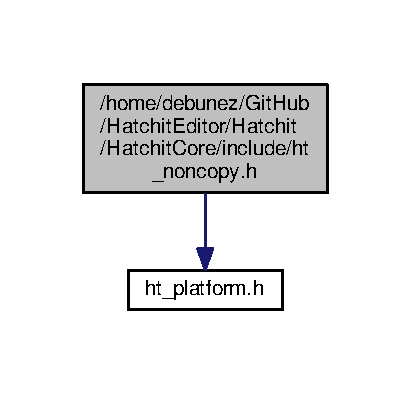
\includegraphics[width=197pt]{ht__noncopy_8h__incl}
\end{center}
\end{figure}
This graph shows which files directly or indirectly include this file\+:
\nopagebreak
\begin{figure}[H]
\begin{center}
\leavevmode
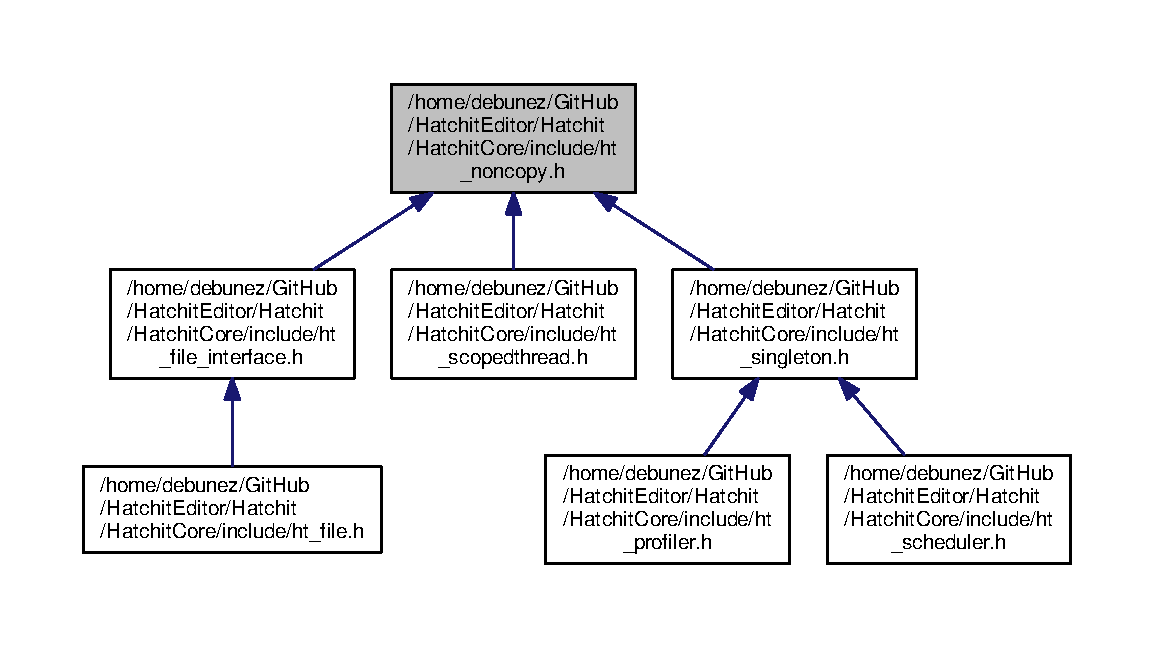
\includegraphics[width=350pt]{ht__noncopy_8h__dep__incl}
\end{center}
\end{figure}
\subsection*{Classes}
\begin{DoxyCompactItemize}
\item 
interface \hyperlink{classHatchit_1_1Core_1_1INonCopy}{Hatchit\+::\+Core\+::\+I\+Non\+Copy}
\begin{DoxyCompactList}\small\item\em Describes a class that cannot be copied. \end{DoxyCompactList}\end{DoxyCompactItemize}
\subsection*{Namespaces}
\begin{DoxyCompactItemize}
\item 
 \hyperlink{namespaceHatchit}{Hatchit}
\begin{DoxyCompactList}\small\item\em Engine global layer. \end{DoxyCompactList}\item 
 \hyperlink{namespaceHatchit_1_1Core}{Hatchit\+::\+Core}
\begin{DoxyCompactList}\small\item\em Engine utility layer. \end{DoxyCompactList}\end{DoxyCompactItemize}


\subsection{Detailed Description}
\hyperlink{namespaceHatchit}{Hatchit} Engine Copyright(c) 2015-\/2016 Third-\/\+Degree

G\+NU Lesser General Public License This file may be used under the terms of the G\+NU Lesser General Public License version 3 as published by the Free Software Foundation and appearing in the file L\+I\+C\+E\+N\+S\+E.\+L\+G\+P\+Lv3 included in the packaging of this file. Please review the following information to ensure the G\+NU Lesser General Public License requirements will be met\+: \href{https://www.gnu.org/licenses/lgpl.html}{\tt https\+://www.\+gnu.\+org/licenses/lgpl.\+html} Noncopy Interface

This file contains the interface definition for noncopyable classes 
\hypertarget{ht__os_8h}{}\section{/home/debunez/\+Git\+Hub/\+Hatchit\+Editor/\+Hatchit/\+Hatchit\+Core/include/ht\+\_\+os.h File Reference}
\label{ht__os_8h}\index{/home/debunez/\+Git\+Hub/\+Hatchit\+Editor/\+Hatchit/\+Hatchit\+Core/include/ht\+\_\+os.\+h@{/home/debunez/\+Git\+Hub/\+Hatchit\+Editor/\+Hatchit/\+Hatchit\+Core/include/ht\+\_\+os.\+h}}
{\ttfamily \#include $<$ht\+\_\+platform.\+h$>$}\\*
{\ttfamily \#include $<$string$>$}\\*
Include dependency graph for ht\+\_\+os.\+h\+:
\nopagebreak
\begin{figure}[H]
\begin{center}
\leavevmode
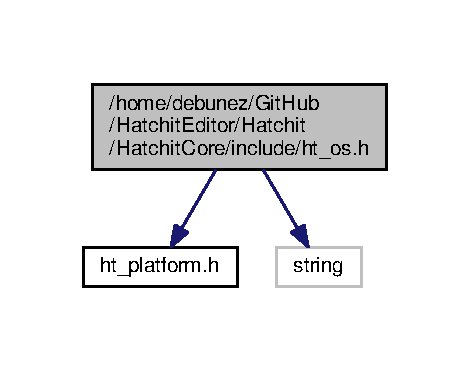
\includegraphics[width=226pt]{ht__os_8h__incl}
\end{center}
\end{figure}
\subsection*{Namespaces}
\begin{DoxyCompactItemize}
\item 
 \hyperlink{namespaceHatchit}{Hatchit}
\begin{DoxyCompactList}\small\item\em Engine global layer. \end{DoxyCompactList}\item 
 \hyperlink{namespaceHatchit_1_1Core}{Hatchit\+::\+Core}
\begin{DoxyCompactList}\small\item\em Engine utility layer. \end{DoxyCompactList}\end{DoxyCompactItemize}
\subsection*{Functions}
\begin{DoxyCompactItemize}
\item 
H\+T\+\_\+\+A\+PI void {\bfseries Hatchit\+::\+Core\+::os\+\_\+mkdir} (const std\+::string \&path)\hypertarget{namespaceHatchit_1_1Core_ada6dafa34682ddf11a428f1afd087d31}{}\label{namespaceHatchit_1_1Core_ada6dafa34682ddf11a428f1afd087d31}

\item 
H\+T\+\_\+\+A\+PI bool {\bfseries Hatchit\+::\+Core\+::os\+\_\+isdir} (const std\+::string \&path)\hypertarget{namespaceHatchit_1_1Core_af5539c53cda834892639880ce83f07b2}{}\label{namespaceHatchit_1_1Core_af5539c53cda834892639880ce83f07b2}

\item 
H\+T\+\_\+\+A\+PI std\+::string {\bfseries Hatchit\+::\+Core\+::os\+\_\+path} (const std\+::string \&path)\hypertarget{namespaceHatchit_1_1Core_a475971d07c33df39e7fe4b72f9e4f021}{}\label{namespaceHatchit_1_1Core_a475971d07c33df39e7fe4b72f9e4f021}

\item 
H\+T\+\_\+\+A\+PI std\+::string {\bfseries Hatchit\+::\+Core\+::os\+\_\+dir} (const std\+::string \&path, bool wt=true)\hypertarget{namespaceHatchit_1_1Core_a3e275c86e7b5fc6a1efad72ddce1ef43}{}\label{namespaceHatchit_1_1Core_a3e275c86e7b5fc6a1efad72ddce1ef43}

\item 
H\+T\+\_\+\+A\+PI std\+::string {\bfseries Hatchit\+::\+Core\+::os\+\_\+exec\+\_\+dir} ()\hypertarget{namespaceHatchit_1_1Core_a723c20b12c91d492e3b05e8180a0c924}{}\label{namespaceHatchit_1_1Core_a723c20b12c91d492e3b05e8180a0c924}

\item 
H\+T\+\_\+\+A\+PI char {\bfseries Hatchit\+::\+Core\+::os\+\_\+path\+\_\+delimeter} ()\hypertarget{namespaceHatchit_1_1Core_aa8dd5e72b88d07efb7016f5c599b2f93}{}\label{namespaceHatchit_1_1Core_aa8dd5e72b88d07efb7016f5c599b2f93}

\end{DoxyCompactItemize}


\subsection{Detailed Description}
\hyperlink{namespaceHatchit}{Hatchit} Engine Copyright(c) 2015-\/2016 Third-\/\+Degree

G\+NU Lesser General Public License This file may be used under the terms of the G\+NU Lesser General Public License version 3 as published by the Free Software Foundation and appearing in the file L\+I\+C\+E\+N\+S\+E.\+L\+G\+P\+Lv3 included in the packaging of this file. Please review the following information to ensure the G\+NU Lesser General Public License requirements will be met\+: \href{https://www.gnu.org/licenses/lgpl.html}{\tt https\+://www.\+gnu.\+org/licenses/lgpl.\+html} Operating System Utilities

This file contains utility functions for operating system tasks, and each function is defined to be cross platform. 
\hypertarget{ht__singleton_8h}{}\section{/home/debunez/\+Git\+Hub/\+Hatchit\+Editor/\+Hatchit/\+Hatchit\+Core/include/ht\+\_\+singleton.h File Reference}
\label{ht__singleton_8h}\index{/home/debunez/\+Git\+Hub/\+Hatchit\+Editor/\+Hatchit/\+Hatchit\+Core/include/ht\+\_\+singleton.\+h@{/home/debunez/\+Git\+Hub/\+Hatchit\+Editor/\+Hatchit/\+Hatchit\+Core/include/ht\+\_\+singleton.\+h}}


Singelton class definition.  


{\ttfamily \#include $<$ht\+\_\+platform.\+h$>$}\\*
{\ttfamily \#include $<$ht\+\_\+noncopy.\+h$>$}\\*
{\ttfamily \#include $<$type\+\_\+traits$>$}\\*
{\ttfamily \#include $<$ht\+\_\+singleton.\+inl$>$}\\*
Include dependency graph for ht\+\_\+singleton.\+h\+:
\nopagebreak
\begin{figure}[H]
\begin{center}
\leavevmode
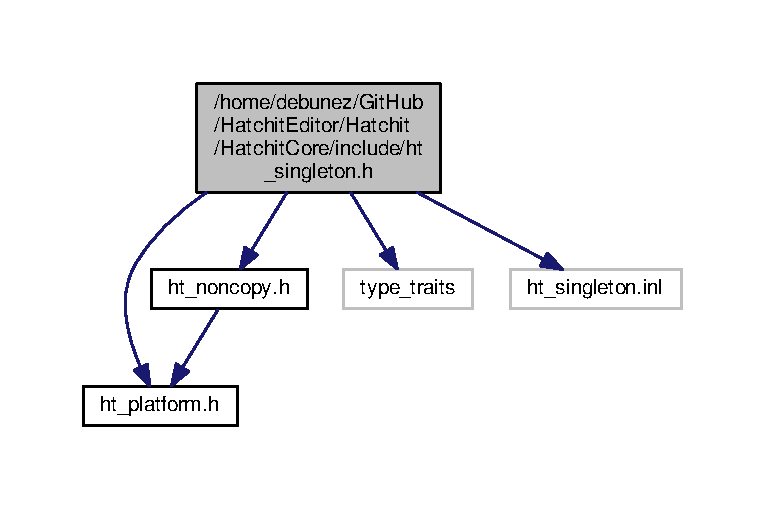
\includegraphics[width=350pt]{ht__singleton_8h__incl}
\end{center}
\end{figure}
This graph shows which files directly or indirectly include this file\+:
\nopagebreak
\begin{figure}[H]
\begin{center}
\leavevmode
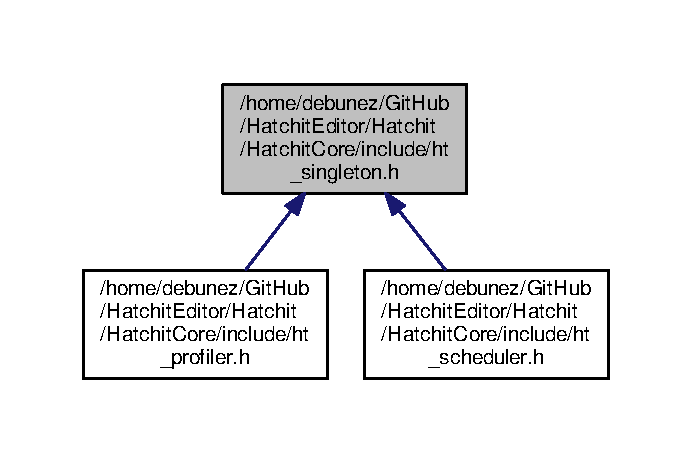
\includegraphics[width=332pt]{ht__singleton_8h__dep__incl}
\end{center}
\end{figure}
\subsection*{Classes}
\begin{DoxyCompactItemize}
\item 
class \hyperlink{classHatchit_1_1Core_1_1Singleton}{Hatchit\+::\+Core\+::\+Singleton$<$ T $>$}
\begin{DoxyCompactList}\small\item\em Describes class that has only one instance avialable globally. \end{DoxyCompactList}\end{DoxyCompactItemize}
\subsection*{Namespaces}
\begin{DoxyCompactItemize}
\item 
 \hyperlink{namespaceHatchit}{Hatchit}
\begin{DoxyCompactList}\small\item\em Engine global layer. \end{DoxyCompactList}\item 
 \hyperlink{namespaceHatchit_1_1Core}{Hatchit\+::\+Core}
\begin{DoxyCompactList}\small\item\em Engine utility layer. \end{DoxyCompactList}\end{DoxyCompactItemize}


\subsection{Detailed Description}
Singelton class definition. 

\hyperlink{namespaceHatchit}{Hatchit} Engine Copyright(c) 2015-\/2016 Third-\/\+Degree

G\+NU Lesser General Public License This file may be used under the terms of the G\+NU Lesser General Public License version 3 as published by the Free Software Foundation and appearing in the file L\+I\+C\+E\+N\+S\+E.\+L\+G\+P\+Lv3 included in the packaging of this file. Please review the following information to ensure the G\+NU Lesser General Public License requirements will be met\+: \href{https://www.gnu.org/licenses/lgpl.html}{\tt https\+://www.\+gnu.\+org/licenses/lgpl.\+html}

\begin{DoxyAuthor}{Author}
Matt Guerrette (\href{mailto:direct3Dtutorials@gmail.com}{\tt direct3\+Dtutorials@gmail.\+com}) 

Third-\/\+Degree contributors (\href{https://github.com/thirddegree}{\tt https\+://github.\+com/thirddegree})
\end{DoxyAuthor}
This file contains definition for Singleton class 
\hypertarget{ht__threadvector_8h}{}\section{/home/debunez/\+Git\+Hub/\+Hatchit\+Editor/\+Hatchit/\+Hatchit\+Core/include/ht\+\_\+threadvector.h File Reference}
\label{ht__threadvector_8h}\index{/home/debunez/\+Git\+Hub/\+Hatchit\+Editor/\+Hatchit/\+Hatchit\+Core/include/ht\+\_\+threadvector.\+h@{/home/debunez/\+Git\+Hub/\+Hatchit\+Editor/\+Hatchit/\+Hatchit\+Core/include/ht\+\_\+threadvector.\+h}}


Threadsafe\+Vector class definition.  


{\ttfamily \#include $<$ht\+\_\+platform.\+h$>$}\\*
{\ttfamily \#include $<$vector$>$}\\*
{\ttfamily \#include $<$mutex$>$}\\*
{\ttfamily \#include $<$memory$>$}\\*
{\ttfamily \#include $<$cassert$>$}\\*
{\ttfamily \#include $<$ht\+\_\+threadvector.\+inl$>$}\\*
Include dependency graph for ht\+\_\+threadvector.\+h\+:
\nopagebreak
\begin{figure}[H]
\begin{center}
\leavevmode
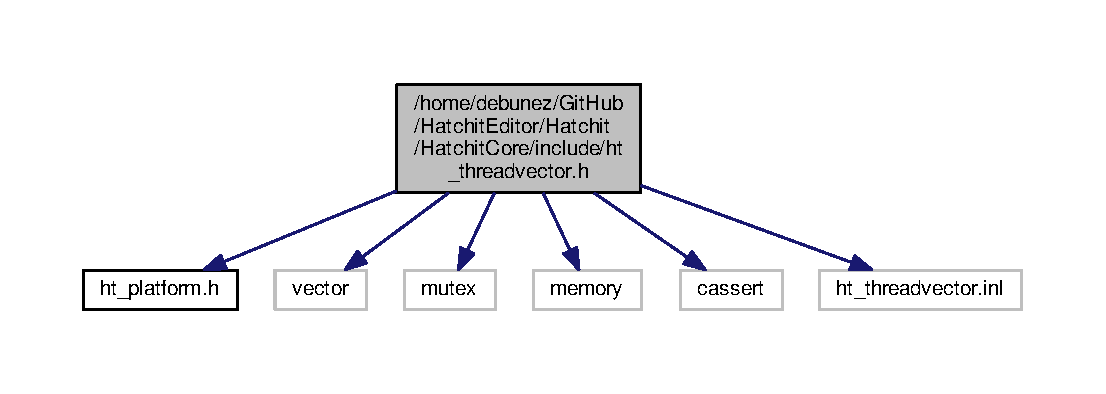
\includegraphics[width=350pt]{ht__threadvector_8h__incl}
\end{center}
\end{figure}
\subsection*{Classes}
\begin{DoxyCompactItemize}
\item 
class \hyperlink{classHatchit_1_1Core_1_1ThreadsafeVector}{Hatchit\+::\+Core\+::\+Threadsafe\+Vector$<$ T $>$}
\begin{DoxyCompactList}\small\item\em wrapper for std\+::vector that provides thread-\/safe functions \end{DoxyCompactList}\end{DoxyCompactItemize}
\subsection*{Namespaces}
\begin{DoxyCompactItemize}
\item 
 \hyperlink{namespaceHatchit}{Hatchit}
\begin{DoxyCompactList}\small\item\em Engine global layer. \end{DoxyCompactList}\item 
 \hyperlink{namespaceHatchit_1_1Core}{Hatchit\+::\+Core}
\begin{DoxyCompactList}\small\item\em Engine utility layer. \end{DoxyCompactList}\end{DoxyCompactItemize}


\subsection{Detailed Description}
Threadsafe\+Vector class definition. 

\hyperlink{namespaceHatchit}{Hatchit} Engine Copyright(c) 2015-\/2016 Third-\/\+Degree

G\+NU Lesser General Public License This file may be used under the terms of the G\+NU Lesser General Public License version 3 as published by the Free Software Foundation and appearing in the file L\+I\+C\+E\+N\+S\+E.\+L\+G\+P\+Lv3 included in the packaging of this file. Please review the following information to ensure the G\+NU Lesser General Public License requirements will be met\+: \href{https://www.gnu.org/licenses/lgpl.html}{\tt https\+://www.\+gnu.\+org/licenses/lgpl.\+html}

\begin{DoxyAuthor}{Author}
Matt Guerrette (\href{mailto:direct3Dtutorials@gmail.com}{\tt direct3\+Dtutorials@gmail.\+com}) 

Third-\/\+Degree contributors (\href{https://github.com/thirddegree}{\tt https\+://github.\+com/thirddegree})
\end{DoxyAuthor}
This file contains definition for Threadsafe\+Vector class 
\hypertarget{ht__timer_8h}{}\section{/home/debunez/\+Git\+Hub/\+Hatchit\+Editor/\+Hatchit/\+Hatchit\+Core/include/ht\+\_\+timer.h File Reference}
\label{ht__timer_8h}\index{/home/debunez/\+Git\+Hub/\+Hatchit\+Editor/\+Hatchit/\+Hatchit\+Core/include/ht\+\_\+timer.\+h@{/home/debunez/\+Git\+Hub/\+Hatchit\+Editor/\+Hatchit/\+Hatchit\+Core/include/ht\+\_\+timer.\+h}}


Timer interface.  


{\ttfamily \#include $<$ht\+\_\+platform.\+h$>$}\\*
Include dependency graph for ht\+\_\+timer.\+h\+:
\nopagebreak
\begin{figure}[H]
\begin{center}
\leavevmode
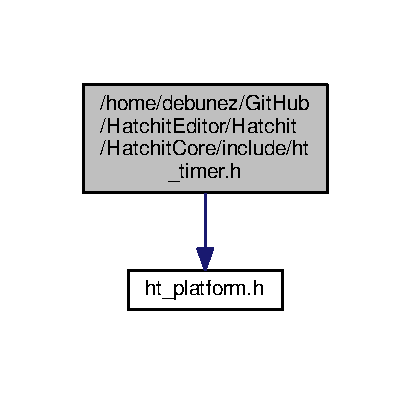
\includegraphics[width=197pt]{ht__timer_8h__incl}
\end{center}
\end{figure}
This graph shows which files directly or indirectly include this file\+:
\nopagebreak
\begin{figure}[H]
\begin{center}
\leavevmode
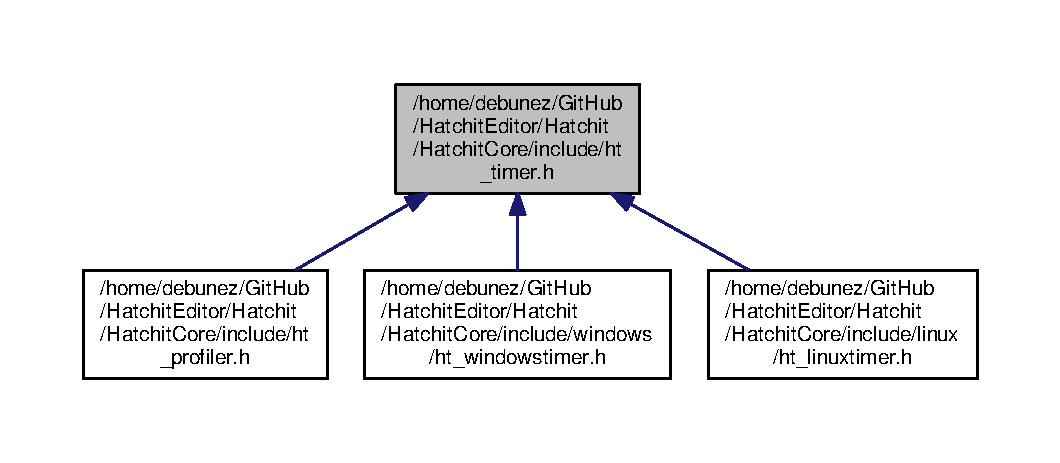
\includegraphics[width=350pt]{ht__timer_8h__dep__incl}
\end{center}
\end{figure}
\subsection*{Classes}
\begin{DoxyCompactItemize}
\item 
interface \hyperlink{classHatchit_1_1Core_1_1ITimer}{Hatchit\+::\+Core\+::\+I\+Timer}
\begin{DoxyCompactList}\small\item\em Interface to describe timer functionality. \end{DoxyCompactList}\end{DoxyCompactItemize}
\subsection*{Namespaces}
\begin{DoxyCompactItemize}
\item 
 \hyperlink{namespaceHatchit}{Hatchit}
\begin{DoxyCompactList}\small\item\em Engine global layer. \end{DoxyCompactList}\item 
 \hyperlink{namespaceHatchit_1_1Core}{Hatchit\+::\+Core}
\begin{DoxyCompactList}\small\item\em Engine utility layer. \end{DoxyCompactList}\end{DoxyCompactItemize}


\subsection{Detailed Description}
Timer interface. 

\hyperlink{namespaceHatchit}{Hatchit} Engine Copyright(c) 2016 Third-\/\+Degree

G\+NU Lesser General Public License This file may be used under the terms of the G\+NU Lesser General Public License version 3 as published by the Free Software Foundation and appearing in the file L\+I\+C\+E\+N\+S\+E.\+L\+G\+P\+Lv3 included in the packaging of this file. Please review the following information to ensure the G\+NU Lesser General Public License requirements will be met\+: \href{https://www.gnu.org/licenses/lgpl.html}{\tt https\+://www.\+gnu.\+org/licenses/lgpl.\+html}

\begin{DoxyAuthor}{Author}
Matt Guerrette (\href{mailto:direct3Dtutorials@gmail.com}{\tt direct3\+Dtutorials@gmail.\+com}) 

Third-\/\+Degree contributors (\href{https://github.com/thirddegree}{\tt https\+://github.\+com/thirddegree})
\end{DoxyAuthor}
This file contains definition for Timer interface 
\hypertarget{ht__linuxtimer_8h}{}\section{/home/debunez/\+Git\+Hub/\+Hatchit\+Editor/\+Hatchit/\+Hatchit\+Core/include/linux/ht\+\_\+linuxtimer.h File Reference}
\label{ht__linuxtimer_8h}\index{/home/debunez/\+Git\+Hub/\+Hatchit\+Editor/\+Hatchit/\+Hatchit\+Core/include/linux/ht\+\_\+linuxtimer.\+h@{/home/debunez/\+Git\+Hub/\+Hatchit\+Editor/\+Hatchit/\+Hatchit\+Core/include/linux/ht\+\_\+linuxtimer.\+h}}


Timer class definition.  


{\ttfamily \#include $<$ht\+\_\+platform.\+h$>$}\\*
{\ttfamily \#include $<$ht\+\_\+timer.\+h$>$}\\*
{\ttfamily \#include $<$time.\+h$>$}\\*
Include dependency graph for ht\+\_\+linuxtimer.\+h\+:
\nopagebreak
\begin{figure}[H]
\begin{center}
\leavevmode
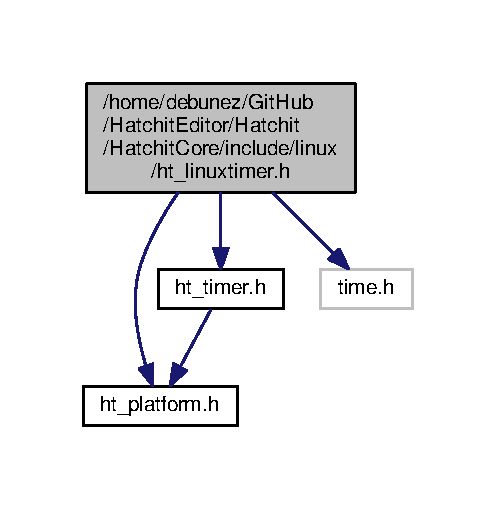
\includegraphics[width=238pt]{ht__linuxtimer_8h__incl}
\end{center}
\end{figure}
\subsection*{Classes}
\begin{DoxyCompactItemize}
\item 
class \hyperlink{classHatchit_1_1Core_1_1Linux_1_1Timer}{Hatchit\+::\+Core\+::\+Linux\+::\+Timer}
\begin{DoxyCompactList}\small\item\em Defines class to track elapsed time. \end{DoxyCompactList}\end{DoxyCompactItemize}
\subsection*{Namespaces}
\begin{DoxyCompactItemize}
\item 
 \hyperlink{namespaceHatchit}{Hatchit}
\begin{DoxyCompactList}\small\item\em Engine global layer. \end{DoxyCompactList}\item 
 \hyperlink{namespaceHatchit_1_1Core}{Hatchit\+::\+Core}
\begin{DoxyCompactList}\small\item\em Engine utility layer. \end{DoxyCompactList}\item 
 \hyperlink{namespaceLinux}{Linux}
\begin{DoxyCompactList}\small\item\em Engine \hyperlink{namespaceLinux}{Linux} platform utilities. \end{DoxyCompactList}\end{DoxyCompactItemize}


\subsection{Detailed Description}
Timer class definition. 

\hyperlink{namespaceHatchit}{Hatchit} Engine Copyright(c) 2016 Third-\/\+Degree

G\+NU Lesser General Public License This file may be used under the terms of the G\+NU Lesser General Public License version 3 as published by the Free Software Foundation and appearing in the file L\+I\+C\+E\+N\+S\+E.\+L\+G\+P\+Lv3 included in the packaging of this file. Please review the following information to ensure the G\+NU Lesser General Public License requirements will be met\+: \href{https://www.gnu.org/licenses/lgpl.html}{\tt https\+://www.\+gnu.\+org/licenses/lgpl.\+html}

\begin{DoxyAuthor}{Author}
Matt Guerrette (\href{mailto:direct3Dtutorials@gmail.com}{\tt direct3\+Dtutorials@gmail.\+com}) 

Third-\/\+Degree contibutors (\href{https://github.com/thirddegree}{\tt https\+://github.\+com/thirddegree})
\end{DoxyAuthor}
This file contains definition for \hyperlink{namespaceLinux}{Linux} Timer class 
\hypertarget{ht__windowstimer_8h}{}\section{/home/debunez/\+Git\+Hub/\+Hatchit\+Editor/\+Hatchit/\+Hatchit\+Core/include/windows/ht\+\_\+windowstimer.h File Reference}
\label{ht__windowstimer_8h}\index{/home/debunez/\+Git\+Hub/\+Hatchit\+Editor/\+Hatchit/\+Hatchit\+Core/include/windows/ht\+\_\+windowstimer.\+h@{/home/debunez/\+Git\+Hub/\+Hatchit\+Editor/\+Hatchit/\+Hatchit\+Core/include/windows/ht\+\_\+windowstimer.\+h}}


Timer class definition.  


{\ttfamily \#include $<$ht\+\_\+platform.\+h$>$}\\*
{\ttfamily \#include $<$ht\+\_\+timer.\+h$>$}\\*
Include dependency graph for ht\+\_\+windowstimer.\+h\+:
\nopagebreak
\begin{figure}[H]
\begin{center}
\leavevmode
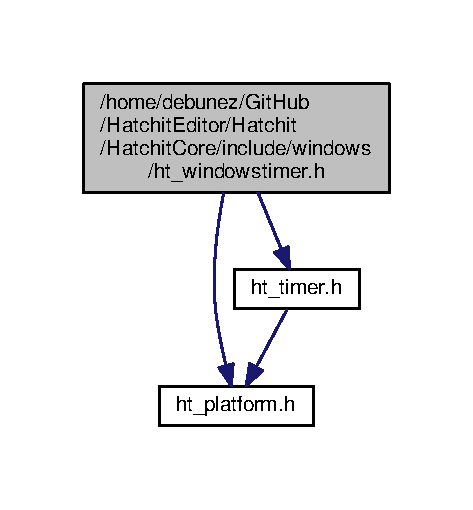
\includegraphics[width=227pt]{ht__windowstimer_8h__incl}
\end{center}
\end{figure}
\subsection*{Classes}
\begin{DoxyCompactItemize}
\item 
class \hyperlink{classHatchit_1_1Core_1_1Windows_1_1Timer}{Hatchit\+::\+Core\+::\+Windows\+::\+Timer}
\begin{DoxyCompactList}\small\item\em Defines class to track elapsed time. \end{DoxyCompactList}\end{DoxyCompactItemize}
\subsection*{Namespaces}
\begin{DoxyCompactItemize}
\item 
 \hyperlink{namespaceHatchit}{Hatchit}
\begin{DoxyCompactList}\small\item\em Engine global layer. \end{DoxyCompactList}\item 
 \hyperlink{namespaceHatchit_1_1Core}{Hatchit\+::\+Core}
\begin{DoxyCompactList}\small\item\em Engine utility layer. \end{DoxyCompactList}\item 
 \hyperlink{namespaceWindows}{Windows}
\begin{DoxyCompactList}\small\item\em Engine \hyperlink{namespaceWindows}{Windows} platform utilities. \end{DoxyCompactList}\end{DoxyCompactItemize}


\subsection{Detailed Description}
Timer class definition. 

\hyperlink{namespaceHatchit}{Hatchit} Engine Copyright(c) 2016 Third-\/\+Degree

G\+NU Lesser General Public License This file may be used under the terms of the G\+NU Lesser General Public License version 3 as published by the Free Software Foundation and appearing in the file L\+I\+C\+E\+N\+S\+E.\+L\+G\+P\+Lv3 included in the packaging of this file. Please review the following information to ensure the G\+NU Lesser General Public License requirements will be met\+: \href{https://www.gnu.org/licenses/lgpl.html}{\tt https\+://www.\+gnu.\+org/licenses/lgpl.\+html}

\begin{DoxyAuthor}{Author}
Matt Guerrette (\href{mailto:direct3Dtutorials@gmail.com}{\tt direct3\+Dtutorials@gmail.\+com}) 

Third-\/\+Degree contributors (\href{https://github.com/thirddegree}{\tt https\+://github.\+com/thirddegree})
\end{DoxyAuthor}
This file contains definition for \hyperlink{namespaceWindows}{Windows} Timer class 
%--- End generated contents ---

% Index
\backmatter
\newpage
\phantomsection
\clearemptydoublepage
\addcontentsline{toc}{chapter}{Index}
\printindex

\end{document}
